\documentclass[a4paper,12pt]{article}
\usepackage{fontspec}
\usepackage{xeCJK}
%\usepackage{helvet}
%\setCJKmainfont{SimSun}
\setmainfont{Times New Roman}
%\setmainfont{helvet}
\usepackage[english]{babel}
%\usepackage[utf8]{inputenc}

%\usepackage[T1]{fontenc}
\usepackage{amsmath}
\usepackage{amsthm}
\usepackage{amsfonts}
\usepackage{amssymb}
\usepackage{graphicx}
\usepackage{hyperref}
\usepackage{enumitem}
\usepackage{textcomp}
\usepackage{float}
\usepackage{booktabs}
%\usepackage{CJKutf8}

\usepackage[colorinlistoftodos]{todonotes}
\usepackage[left=1.50cm, right=1.50cm, top=1.20cm]{geometry}
\linespread{1.5}
\usepackage{algorithm}
\usepackage{algpseudocode}
\usepackage{fancybox}
\usepackage{tikz}
\usepackage[tikz]{mdframed}
\usetikzlibrary{matrix, positioning, fit, arrows, calc, intersections, shapes, shadings, patterns, decorations.markings, chains, scopes, shapes.arrows, trees}

\usepackage{upquote}
\usepackage{listings}
\usepackage{url}
\lstset{upquote=true}
\lstdefinestyle{customc}{
  belowcaptionskip=1\baselineskip,
  breaklines=true,
  frame=L,
  xleftmargin=\parindent,
  language=C++,
  tabsize=2,
  showstringspaces=false,
  basicstyle=\small\ttfamily,
  keywordstyle=\bfseries\color{green!40!black},
  commentstyle=\itshape\color{purple!40!black},
  identifierstyle=\color{blue},
  stringstyle=\color{orange},
}
\mdfdefinestyle{mymdf}{leftmargin=1cm,rightmargin=2cm,%
innerleftmargin=1cm,innerrightmargin=1cm,roundcorner=10pt,backgroundcolor=lg}
\definecolor{lg}{RGB}{247,249,250}
\title{Algorithm Problem Set \\ \large No. 001 --- 100}
%\title{Functional Programming In C++}
\author{SS}
\date{November 2018}

\begin{document}
\def\bottom#1#2{\hbox{\vbox to #1{\vfill\hbox{#2}}}}
%\fontfamily{phv}\selectfont
\renewcommand{\thelstlisting}{\thesection.\arabic{lstlisting}}
\sloppy
\maketitle
\section{400 --- Nth Digit}
Find the $n$th digit of the infinite integer sequence 1, 2, 3, 4, 5, 6, 7, 8, 9, 10, 11, $\ldots$

\paragraph{Note:}
\begin{itemize}
\item $ n $ is positive and will fit within the range of a 32-bit signed integer ($n < 2^{31}$).
\end{itemize}

\paragraph{Example 1:}

\begin{flushleft}
\textbf{Input}: 3
\textbf{Output}: 3
\end{flushleft}

\paragraph{Example 2:}

\begin{flushleft}
\textbf{Input}: 11
\textbf{Output}: 0
\textbf{Explanation}:
\\
The 11th digit of the sequence 1, 2, 3, 4, 5, 6, 7, 8, 9, 10, 11, $\ldots$ is a 0, which is part of the number 10.
\end{flushleft}

\subsection{Mathematical Induction}
问题可以分为三个部分
\begin{enumerate}
\item 计算包含第$n$个digit的number $x$是几位数。
\item 找到$x$。
\item 找到包含在$x$中的第$n$个digit
\end{enumerate}
例如,假设需要找到第250个digit,
\begin{enumerate}
\item 很容易找到$x$是三位数,因为1--9有9个数字,而10--99有180个数字,$250 - 9 - 90 \times 2 = 61$。即$n$是3位数中从100开始的第61个数字。
\item 找到$x$: 由于计数是从1开始,所以$x=100+(61-1)/3=120$。
\item 最后在$x$中找到第$n$th digit: 因为$(n-1)\bmod 3=0$,所以$x$中第0个数字即为$n$th digit。即1。
\end{enumerate}

\setcounter{lstlisting}{0}
\begin{lstlisting}[style=customc, caption={Mathematical Induction}]
int findNthDigit( int n )
{
    long long base = 9;
    long long z = 1; //number of digits
    long long start = 1; // start=1,10,100,....

    auto ln = static_cast<long long>( n );

    while( ln > base * z )
    {
        ln -= base * z;
        base *= 10;
        ++z;
        start *= 10;
    }

    //get number x that contains nth digit
    auto x = start + ( ( ln - 1 ) / z );

    //get the index of nth digit in x
    //from left to right
    auto i = ( ( ln - 1 ) % z );

    //convert to string
    auto s = to_string( x );

    return s[i] - '0';

}
\end{lstlisting}

\section{401 --- Binary Watch}
A binary watch has 4 LEDs on the top which represent the hours (0--11), and the 6 LEDs on the bottom represent the minutes (0--59).
\par
Each LED represents a zero or one, with the least significant bit on the right. So the 4 LEDs represent hours 8, 4, 2 and 1. The 6 LEDs represent the minutes 32, 16, 8, 4, 2 and 1 respectively.
\par
Given a non-negative integer $ n $ which represents the number of LEDs that are currently on, return all possible times the watch could represent.

\paragraph{Example:}

\begin{flushleft}
\textbf{Input}: $ n = 1 $
\\
\textbf{Output}: [ 1:00, 2:00, 4:00, 8:00, 0:01, 0:02, 0:04, 0:08, 0:16, 0:32 ]

\end{flushleft}

\paragraph{Note:}

\begin{itemize}
\item  The order of output does not matter.
\item The hour must not contain a leading zero, for example 01:00 is not valid, it should be 1:00.
\item The minute must be consist of two digits and may contain a leading zero, for example 10:2 is not valid, it should be 10:02.
\end{itemize}

\subsection{Combination}
总共要取$n$个,首先在代表hours的4个LEDs里面取$h$个,然后在代表minutes的6个LEDs里面取$n-h$个,分别对hours和minutes进行递归处理,然后将符合范围的hour和minute组合起来,放入输出array中。

\setcounter{lstlisting}{0}
\begin{lstlisting}[style=customc, caption={Combination}]
vector<string> readBinaryWatch( int num )
{
    const int hours[4] = {8, 4, 2, 1};
    const int minutes[6] = {32, 16, 8, 4, 2, 1};

    vector<string> ans;
    for( int h = 0; h <= num; ++h )
    {
        //get all possible hours for h leds
        vector<int> hs;
        dfs( hours, 4, 0, h, 0, hs );

        //get all possible minutes for (n-h) leds
        vector<int> ms;
        dfs( minutes, 6, 0, num - h, 0, ms );

        for( auto x : hs )
        {
            if( ( x >= 0 ) && ( x <= 11 ) )
            {
                //hour is between [0,11]
                for( auto y : ms )
                {
                    if( ( y >= 0 ) && ( y <= 59 ) )
                    {
                        //minute is between [0,59]
                        string s_time = to_string( x );
                        s_time.push_back( ':' );
                        //make sure minute has leading zero for [0,9]
                        s_time += ( y < 10 ) ? ( "0" + to_string( y ) ) : to_string( y );
                        ans.emplace_back( s_time );
                    }
                }//end for
            } //end if
        } //end for
    }

    return ans;
}

//helper function: recursively genenrate hours with *count* leds
void dfs( const int* a, int len, int start, int count, int t, vector<int>& res )
{
    if( count == 0 )
    {
        //we have already used *count* leds
        res.push_back( t );
        return;
    }

    for( int i = start; i < len; ++i )
    {
        //since this is combination
        //try next from (i+1)
        dfs( a, len, i + 1, count - 1, t + a[i], res );
    }
}
\end{lstlisting}
\section{402 --- Remove K Digits}
Given a non-negative integer $n$ represented as a string, remove $k$ digits from the number so that the new number is the smallest possible.
\par
\paragraph{Note:}

\begin{itemize}
\item     The length of $ n $ is less than 10002 and will be no less than $ k $.
\item     The given $ n $ does not contain any leading zero.

\end{itemize}

\paragraph{Example 1:}

\begin{flushleft}
\textbf{Input}: $n = 1432219$, $k = 3$
\\
\textbf{Output}: $1219$
\\
\textbf{Explanation}: Remove the three digits 4, 3, and 2 to form the new number 1219 which is the smallest.
\end{flushleft}

\paragraph{Example 2:}

\begin{flushleft}
\textbf{Input}: $n = 10200$, $k = 1$
\\
\textbf{Output}: 200
\\
\textbf{Explanation}: Remove the leading 1 and the number is 200. Note that the output must not contain leading zeroes.
\end{flushleft}

\paragraph{Example 3:}

\begin{flushleft}
\textbf{Input}: $n = 10$, $k = 2$
\\
\textbf{Output}: 0
\\
\textbf{Explanation}: Remove all the digits from the number and it is left with nothing which is 0.

\end{flushleft}

\subsection{Sliding Window}
\begin{itemize}
\item 采用sliding window的方法,maintain a double end queue: $q$
\item 从头开始遍历$ n $,将第一个字符放入结果$q$中,然后继续,如果当前digit比$q$中的最后一个digit要大,从$q$中移除最后一个digit,直至$q$为空或者在当前$q$的最后digit不大于当前digit。同时记录从$q$中remove last digit的次数 $\delta$,如果$\delta=k$,就不能再remove last digit了。
\item Remove $q$ 中可能的leading zeros。
\item 最后,$q$中包含的digit个数可能会大于$n$的长度$\ell$减去$k$。原因是$n$中可能会有很多重复的比较小的digit。只需要从$q$中返回$\ell-k$个digits即可。
\end{itemize}

\setcounter{algorithm}{0}
\begin{algorithm}[H]
\caption{Sliding Window}
\begin{algorithmic}[1]
\Procedure{RemoveKdigits}{$n, \ell, k$}
\State $\star$ Maintain a double end queue $q$
\State $\delta:=0$ \Comment The count of removing digits
\For{$i:=0$ \textbf{to} $\ell-1$}
\State $d:=n[i]$
\While{$q$ is not empty \textbf{and} $\delta < k$ \textbf{and} $q$'s last digit is less than $d$}
\State $\star$ Remove last digit from $q$
\State $\delta\gets\delta+1$ \Comment Increments the count of removing digits
\EndWhile
\State $\star$ Add $d$ to end of $q$
\EndFor
\State $\ast$ Remove leading zeros from $q$
\While{$q$ is not empty \textbf{and} $q$'s first digit is zero}
\State $\star$ Remove first digit from $q$
\EndWhile
\If{$q$ is empty}
\State \Return 0 \Comment Only zero remains in $q$
\EndIf
\State $l:=\min(\ell-k, \lvert q\rvert)$ \Comment $q$ may contain more than $\ell-k$ digits because of duplicate smaller numbers
\State $s=\emptyset$ \Comment The result number
\For{$x:=0$ \textbf{to} $l-1$}
\State $\star$ Add first digit of $q$ to $s$
\State $\star$ Remove first digit from $q$
\EndFor
\If{$s$ is empty}
\State \Return 0 \Comment All digits are removed from $n$
\Else
\State \Return $s$
\EndIf
\algstore{402algo}
\end{algorithmic}
\end{algorithm}
\begin{algorithm}[H]
\begin{algorithmic}[1]
\algrestore{402algo}
\EndProcedure
\end{algorithmic}
\end{algorithm}

\setcounter{lstlisting}{0}
\begin{lstlisting}[style=customc, caption={Sliding Window}]
string removeKdigits( string num, int k )
{
    deque<char> q;
    //the count of remove digits
    int count = 0;

    //process sliding window
    for( auto c : num )
    {
        while( !q.empty() && ( count < k ) && ( q.back() > c ) )
        {
            q.pop_back();
            ++count;
        }
        q.push_back( c );
    }

    while( !q.empty() && q.front() == '0' )
    {
        q.pop_front();
    }

    if( q.empty() )
    {
        return "0";
    }

    int ln = static_cast<int>( num.size() );
    int lq = static_cast<int>( q.size() );

    //q may contain more than ln-k digits because of duplicate smaller digits
    int total = ( min )( ln - k, lq );

    string ans;

    for( int x = 0; x < total; ++x )
    {
        ans.push_back( q.front() );
        q.pop_front();
    }

    //the result string may still be empty
    //if total is zero
    return ans.empty() ? "0" : ans;
}
\end{lstlisting}
\section{403 --- Frog Jump}
A frog is crossing a river. The river is divided into $x$ units and at each unit there may or may not exist a stone. The frog can jump on a stone, but it must not jump into the water.
\par
Given a list of stones' positions $A$ (in units) in sorted ascending order, determine if the frog is able to cross the river by landing on the last stone. Initially, the frog is on the first stone and assume the first jump must be 1 unit.
\par
If the frog's last jump was $ k $ units, then its next jump must be either $ k - 1 $, $ k $, or $ k + 1 $ units. Note that the frog can only jump in the forward direction.

\paragraph{Note:}

\begin{itemize}
\item The number of stones $2\leq \lvert A\rvert < 1100$
\item Each stone's position will be a non-negative integer $< 2^{31}$.
\item The first stone's position is always 0.
\end{itemize}

\paragraph{Example 1:}
\begin{flushleft}
\textbf{Input}: $[0,1,3,5,6,8,12,17]$
\\
\textbf{Output}: \texttt{true}
\\
\textbf{Explanation}:  There are a total of 8 stones.
\\
The first stone at the 0th unit, second stone at the 1st unit, third stone at the 3rd unit, and so on. The last stone at the 17th unit.
\\
The frog can jump to the last stone by jumping 
1 unit to the 2nd stone, then 2 units to the 3rd stone, then 
2 units to the 4th stone, then 3 units to the 6th stone, 
4 units to the 7th stone, and 5 units to the 8th stone.
\end{flushleft}

\paragraph{Example 2:}

\begin{flushleft}
\textbf{Input}: $[0,1,2,3,4,8,9,11]$
\\
\textbf{Output}: \texttt{false}
\\
\textbf{Explanation}: There is no way to jump to the last stone as the gap between the 5th and 6th stone is too large.
\end{flushleft}

\subsection{Dynamic Programming}
\begin{itemize}
\item Suppose we are at $i$th stone and it take $x$ steps to jump from $(i-1)$th stone to current one.
\item Then from $(i+1)$th stone until last one, if the gap to $i$th stone is between $[x-1,x+1]$, we can jump to that stone. If the gap is larger than $x+1$, we can stop the searching because all stones from this one will not be reachable.
\item For any reachable stone $j$, recursively to find if the frog can jump to the last stone from $j$.
\item To minimize the memory impact, we can use a hash map to memorize. The map's key is the combination of the stone's index $i$ and the steps $x$ that the frog takes to jump from $(i-1)$th stone. We can transform $i$ and $x$ to string and concatenate with a special character such as \# to form the key.
\end{itemize}

\setcounter{lstlisting}{0}
\begin{lstlisting}[style=customc, caption={Dynamic Programming}]
bool canCross( vector<int>& stones )
{
    if( stones.empty() || ( stones.size() == 1 ) )
    {
        return true;
    }

    //make sure the first jump from index 0 to 1
    //can make
    if( stones[1] - stones[0] > 1 )
    {
        //the frog cannot go to the second stone
        return false;
    }
    //memorization for dynamic programming
    unordered_map<string, unsigned char> memo;

    //we start from the second stone, stones[1],
    //the last step is 1 which is from stones[0] to stones[1]
    auto can_jump = dfs( stones, 1, 1, memo );

    return can_jump != 0;
}
//Helper function to find if the frog can jump to last stone starting from ith stone
unsigned char dfs( vector<int>& positions, size_t i, int step, unordered_map<string, unsigned char>& memo )
{
    //form the key
    auto key = to_string( i ) + "#" + to_string( step );

    //find if we already have the value for given stone index (i) and
    //the step from (i-1)th stone
    auto it = memo.find( key );

    if( it != memo.end() )
    {
        return it->second;
    }

    //Can jump to the last stone
    //return true directly
    if( i >= positions.size() - 1 )
    {
        memo.emplace( key, 1 );
        return 1;
    }

    unsigned char can_jump = 0;

    int last_pos = positions[i];

    for( size_t k = i + 1; k < positions.size(); ++k )
    {
        int cur_pos = positions[k];
        //the steps need to take to jump from ith stone
        int gap = cur_pos - last_pos;

        if( gap < step - 1 )
        {
            //too small step
            //skip to next stone
            continue;
        }

        if( gap > step + 1 )
        {
            //too big step
            //break the searching
            break;
        }

        //recursively to check if frog can reach last one
        //when jumping from kth stone
        can_jump = dfs( positions, k, gap, memo );

        if( can_jump == 1 )
        {
            break;
        }
    }

    //add to the memorization
    memo.emplace( key, can_jump );

    return can_jump;
}

\end{lstlisting}
\section{404 --- Sum of Left Leaves}
Find the sum of all left leaves in a given binary tree.

\paragraph{Example:}
\begin{flushleft}
\textbf{Input}:
\begin{figure}[H]
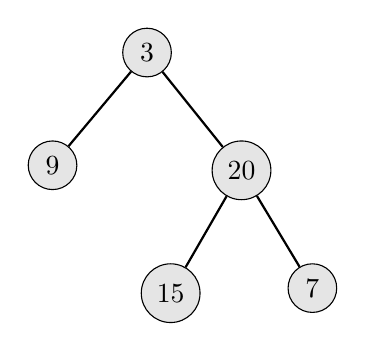
\begin{tikzpicture}
[my/.style={draw, fill=gray!20, circle, minimum size=5mm}]
\node[my](0) at (0,0) {3};
\node[my](1) [below = 8mm of 0, xshift=-12mm] {9};
\node[my](2) [below = 8mm of 0, xshift=12mm] {20};
\node[my](3) [below = 8mm of 2, xshift=-9mm] {15};
\node[my](4) [below = 8mm of 2, xshift=9mm] {7};
\draw[thick] (0) -- (1);
\draw[thick] (0) -- (2);
\draw[thick] (2) -- (3);
\draw[thick] (2) -- (4);
\end{tikzpicture}
\end{figure}
\textbf{Output}: 24
\\
\textbf{Explanation}: There are two left leaves in the binary tree, with values 9 and 15 respectively. Return 24.
\end{flushleft}

\subsection{Depth First Search}
\begin{itemize}
\item We need to add boolean flag as one of parameters in the recursive function to indicate if the current node is left or right.
\item If the root has no child, we must return 0.
\end{itemize}

\setcounter{lstlisting}{0}
\begin{lstlisting}[style=customc, caption={Depth First Search}]
int sumOfLeftLeaves( TreeNode* root )
{

    int ans = 0;

    //if root has no children,
    //we must return 0
    dfs( root, false, ans );

    return ans;
}

//helper function, add is_left to indicate
//if the node is left or right
void dfs( TreeNode* node, bool is_left, int& sum )
{
    if( !node )
    {
        return;
    }

    if( !node->left && !node->right )
    {
        if( is_left )
        {
            //only add sum for left node
            sum += node->val;
        }
    }
    else
    {
        dfs( node->left, true, sum );
        dfs( node->right, false, sum );
    }
}
\end{lstlisting}



\section{405 --- Convert a Number to Hexadecimal}
Given an integer, write an algorithm to convert it to hexadecimal. For negative integer, two’s complement method is used.

\paragraph{Note:}

\begin{itemize}
\item All letters in hexadecimal ($a$--$f$) must be in lowercase.
\item The hexadecimal string must not contain extra leading 0s. If the number is zero, it is represented by a single zero character; otherwise, the first character in the hexadecimal string will not be the zero character.
\item The given number is guaranteed to fit within the range of a 32-bit signed integer.
\item You must not use any method provided by the library which converts/formats the number to hex directly.
\end{itemize}

\paragraph{Example 1:}

\begin{flushleft}
\textbf{Input}: 26
\\
\textbf{Output}: \texttt{1a}
\end{flushleft}

\paragraph{Example 2:}

\begin{flushleft}
\textbf{Input}: $-1$
\\
\textbf{Output}: \texttt{ffffffff}
\end{flushleft}

\subsection{Bit Operation}
\begin{itemize}
\item Basic idea: Right shift the number 4 bits, and then mask with 0xF. 
\item To stop the shift, either the number is zero or the number has been right shifted 8 times. The latter is dealing with the case when number is $-1$. Without latter, the shift will continue forever.
\end{itemize}

\setcounter{lstlisting}{0}
\begin{lstlisting}[style=customc, caption={Bit Manipulation}]
string toHex( int num )
{
    if( num == 0 )
    {
        return "0";
    }

    string hex = "0123456789abcdef";

    int mask = 15;

    string ans;

    int shifts = 0;

    //stop when shift 8 times
    //or num is zero
    while( ( shifts < 8 ) && num )
    {
        ans.push_back( hex[num & mask] );
        num >>= 4;
        ++shifts;
    }

    reverse( ans.begin(), ans.end() );

    return ans;
}
\end{lstlisting}


\section{406 --- Queue Reconstruction by Height}
Suppose you have a random list of people standing in a queue. Each person is described by a pair of integers $(h, k)$, where $h$ is the height of the person and $k$ is the number of people in front of this person who have a height greater than or equal to h. Write an algorithm to reconstruct the queue.

\paragraph{Note:}
\begin{itemize}
\item The number of people is less than 1,100.
\end{itemize}

\paragraph{Example}

\begin{flushleft}
\textbf{Input}: $[\; [7,0], [4,4], [7,1], [5,0], [6,1], [5,2]\;]$
\\
\textbf{Output}: $[\;[5,0], [7,0], [5,2], [6,1], [4,4], [7,1]\;]$
\end{flushleft}

\subsection{Sort}
\begin{itemize}
\item Sort the input list by the height from larger to smaller. If two persons have same heights, the one with smaller $k$ is placed in front.
\item Starting from the second person in the sorted list, maintains a counter $\delta$ that records how many persons in front have a height greater than or equal to current person:
\begin{enumerate}
\item For current person $i$, for any person $j$ in front of $i$, if $h_j \geq h_i$, increments the counter $\delta$. 
\item If $\delta$ equal to $k_i$, from $i-1$ to $j$, we swap each element with its previous one. When this process is completed, put $i$ into $j$ and this will place $i$ into the correct position
\item Then stop and continue to person $i+1$.
\end{enumerate}
\end{itemize}

\begin{lstlisting}[style=customc, caption={Sorting}]
vector<vector<int>> reconstructQueue( vector<vector<int>>& people )
{
    //sort height first from larger to smaller
    //then the order from smaller to larger
    sort( people.begin(), people.end(), []( const vector<int>& p1, const vector<int>&p2 )
    {
        if( p1[0] > p2[0] )
        {
            return true;
        }
        else if( p1[0] == p2[0] )
        {
            return p1[1] < p2[1];
        }

        // return false;
    } );

    int L = static_cast<int>( people.size() );

    for( int i = 1; i < L; ++i )
    {
        //The number of persons in front
        //have a height larger or equal to i
        int z = 0;
        int h = people[i][0];
        int k = people[i][1];

        for( int j = 0; j < i; ++j )
        {

            if( k == z )
            {
                //Found the range of items that need to be replaced

                //copy information from previous item
                for( int x = i - 1; x >= j; --x )
                {
                    people[x + 1][0] = people[x][0];
                    people[x + 1][1] = people[x][1];
                }

                //place i into j
                people[j][0] = h;
                people[j][1] = k;

                break; //stop inner loop
            }

            //increment z
            if( people[j][0] >= h )
            {
                ++z;
            }
        }
    }

    return people;
}
\end{lstlisting}
\section{407 --- Trapping Rain Water II}
Given an $m \times n$ matrix of positive integers representing the height of each unit cell in a 2D elevation map, compute the volume of water it is able to trap after raining.

\paragraph{Note:}

\begin{flushleft}
Both $ m $ and $ n $ are less than 110. The height of each unit cell is greater than 0 and is less than 20,000.

\end{flushleft}
 

\paragraph{Example:}

\begin{flushleft}
Given the following $3\times 6$ height map:
\begin{table}[H]
\begin{tabular}{*{6}{c}}
1 & 4 & 3 & 1 & 3 & 2 \\ 
3 & 2 & 1 & 3 & 2 & 4 \\
2 & 3 & 3 & 2 & 3 & 1
\end{tabular}
\end{table}
Return 4.
\end{flushleft}

\subsection{Priority Queue}
\begin{itemize}
\item Problem 42 是该题的2D形式,解决问题的idea来自于著名的 Liebig's law of the minimum 即 The maximum height of water for current container is determined by the lowest part of its boundary.
\item 算法需要从boundary开始,逐步推进到内部。在这个过程中,首先从bounday最低的部分开始,然后搜索其neighbors,获得其中能够得到的盛水量,然后将其neighbor cell的坐标,和该cell与当前cell的高度相比较更大的那个高度作为cell放入$q$。这个高度形成了新的boundary。
\item 本题是3D形式,因此每个格子都会有四个neighbors,除了边界的以外,因此maintain 一个priority queue $q$,将boundary中所有cell都放入$q$,然后从高度最低的部分开始进行四领域DFS。同时需要maintain 一个 2d array 来mark当前cell是否已经访问过。
\item 由于Priority Queue需要把最小高度的cell放在top,因此这是一个min prority queue。
\end{itemize}

\setcounter{lstlisting}{0}
\begin{lstlisting}[style=customc, caption={Priority Queue}]
int trapRainWater( vector<vector<int>>& heightMap )
{

    if( heightMap.empty() || heightMap[0].empty() )
    {
        return 0;
    }

    int rows = static_cast<int>( heightMap.size() );
    int cols = static_cast<int>( heightMap[0].size() );

    //we need a min priority_queue, so the comparison function
    //need return true for larger one
    auto cmp = []( const cell & c1, const cell & c2 )
    {
        return c1.h > c2.h;
    };

    priority_queue<cell, vector<cell>, decltype( cmp )> pq( cmp );

    //mark if cell at (r,c) is visited or not
    vector<vector<unsigned char>> seen( rows, vector<unsigned char>( cols, 0 ) );

    //put cells on boundaries
    for( int r = 0; r < rows; ++r )
    {
        pq.emplace( r, 0, heightMap[r][0] );
        pq.emplace( r, cols - 1, heightMap[r][cols - 1] );
        seen[r][0] = 1;
        seen[r][cols - 1] = 1;
    }
    for( int c = 1; c < cols - 1; ++c )
    {
        pq.emplace( 0, c, heightMap[0][c] );
        pq.emplace( rows - 1, c, heightMap[rows - 1][c] );
        seen[0][c] = 1;
        seen[rows - 1][c] = 1;
    }

    int dr[4] = {1, 0, -1, 0};
    int dc[4] = {0, 1, 0, -1};

    int ans = 0;
    while( !pq.empty() )
    {
        auto t = pq.top();
        pq.pop();

        for( int i = 0; i < 4; ++i )
        {
            int nr = dr[i] + t.r;
            int nc = dc[i] + t.c;

            if( ( nr < 0 ) || ( nc < 0 ) || ( nr >= rows ) || ( nc >= cols ) )
            {
                continue;
            }

            if( seen[nr][nc] )
            {
                continue;
            }

            int nh = heightMap[nr][nc];

            //only the water is contained
            //if the neighbor height is less
            //than current cell's height
            if( t.h > heightMap[nr][nc] )
            {
                //the new boundary height
                //must be the greater one of
                //current cell and its neighbor
                nh = t.h;
                ans += ( t.h - heightMap[nr][nc] );
            }

            //add the new cell into the queue
            pq.emplace( nr, nc, nh );

            //mark this cell is visited
            seen[nr][nc] = 1;
        }
    }

    return ans;

}

struct cell
{
    int r;
    int c;
    int h;

    cell( int r_, int c_, int h_ )
        : r( r_ ), c( c_ ), h( h_ )
    {}
};
\end{lstlisting}


\section{408 --- Valid Word Abbreviation}
Given a non-empty string $S$ and an abbreviation $T$, return whether the string matches with the given abbreviation.

A string such as \texttt{word} contains only the following valid abbreviations:

[\texttt{word}, \texttt{1ord}, \texttt{w1rd}, \texttt{wo1d}, \texttt{wor1}, \texttt{2rd}, \texttt{w2d}, \texttt{wo2}, \texttt{1o1d}, \texttt{1or1}, \texttt{w1r1}, \texttt{1o2}, \texttt{2r1}, \texttt{3d}, \texttt{w3}, \texttt{4}]

Notice that only the above abbreviations are valid abbreviations of the string word. Any other string is not a valid abbreviation of word.

\paragraph{Note:}

\begin{itemize}
\item Assume $S$ contains only lowercase letters and $T$ contains only lowercase letters and digits.
\end{itemize}

\paragraph{Example 1:}
\begin{flushleft}
\textbf{Input}: $S = \texttt{internationalization}$, $T = \texttt{i12iz4n}$:

\textbf{Output}: \texttt{true}
\end{flushleft}

\paragraph{Example 2:}

\begin{flushleft}
\textbf{Input}: $S = \texttt{apple}$, $T = \texttt{a2e}$:

\textbf{Output}: \texttt{false}
\end{flushleft}

\setcounter{lstlisting}{0}
\begin{lstlisting}[style=customc, caption={Iterative}]
bool validWordAbbreviation( string word, string abbr )
{
    size_t j = 0;
    size_t i = 0;

    while( ( i < word.size() ) && ( j < abbr.size() ) )
    {
        if( ( abbr[j] >= '0' ) && ( abbr[j] <= '9' ) )
        {
            //number starting with zero
            //is invalid
            if( abbr[j] == '0' )
            {
                return false;
            }

            size_t count = 0;

            while( ( j < abbr.size() ) && ( abbr[j] >= '0' ) && ( abbr[j] <= '9' ) )
            {
                count = count * 10 + ( abbr[j] - '0' );
                ++j;
            }

            i += count;
        }
        else
        {
            if( word[i] != abbr[j] )
            {
                //if the lowercase letter
                //is not matched
                //the match is invalid
                return false;
            }

            ++i;
            ++j;
        }
    }
    return ( i == word.size() ) && ( j == abbr.size() );
}
\end{lstlisting}
\section{409 --- Longest Palindrome}
Given a string $S$ which consists of lowercase or uppercase letters, find the length of the longest palindromes that can be built with those letters.
\par
This is case sensitive, for example \texttt{Aa} is not considered a palindrome here.

\paragraph{Note:}
\begin{itemize}
\item Assume the length of given string will not exceed 1,010.
\end{itemize}

\paragraph{Example:}

\begin{flushleft}
\textbf{Input}: \texttt{abccccdd}
\\
\textbf{Output}: 7
\\
\textbf{Explanation}: One longest palindrome that can be built is \texttt{dccaccd}, whose length is 7.
\end{flushleft}

\subsection{Counting}
\begin{itemize}
\item We can only incorporate only one character with largest odd counts into the palindrome even if multiple characters may have same largest odd counts.
\item For any other character with odd counts $x$ , we can incorporate this one with $x-1$ times into the palindrome.
\item The fast way to do this is just add $x-1$ into the result when iterating over the counts array. Also, record the maximum odd counts $y$. At the end, we subtract $(y-1)$ from the result and add back $y$. This is effectively equal to add 1 to the result.
\item Of course, If all characters are have even counts, there is no need to add 1 to the result.
\end{itemize}

\setcounter{lstlisting}{0}
\begin{lstlisting}[style=customc, caption={Counting}]
int longestPalindrome( string s )
{
    //lower case
    int l[26] = {0};
    //uppercase
    int u[26] = {0};

    for( auto c : s )
    {
        if( ( c >= 'a' ) && ( c <= 'z' ) )
        {
            l[c - 'a'] += 1;
        }
        else
        {
            u[c - 'A'] += 1;
        }
    }

    int ans = 0;
    int max_odd_len = 0;
    for( int i = 0; i < 26; ++i )
    {
        if( l[i] & 1 )
        {
            //character i+'a' can be added at least l[i]-1 times
            max_odd_len = ( max )( max_odd_len, l[i] );
            ans += ( l[i] - 1 );
        }
        else
        {
            ans += l[i];
        }

        if( u[i] & 1 )
        {
            //character i+'A' can be added at least u[i]-1 times
            max_odd_len = ( max )( max_odd_len, u[i] );
            ans += ( u[i] - 1 );
        }
        else
        {
            ans += u[i];
        }
    }

    //ans-(max_odd_len-1)+max_odd_len = ans + 1
    //only happens when there exits odd counts characters
    return max_odd_len == 0 ? ans : ans + 1;
}
\end{lstlisting}

\section{410 --- Split Array Largest Sum}
Given an array $A$ which consists of non-negative integers and an integer $ m $, you can split the array into $ m $ non-empty continuous subarrays. Write an algorithm to minimize the largest sum among these $ m $ subarrays.

\paragraph{Note:}
\begin{itemize}
\item If $ n $ is the length of array, assume the following constraints are satisfied:

\begin{enumerate}
\item    $ 1 \leq n \leq 1000$
\item    $ 1 \leq m \leq \min(50, n)$
\end{enumerate}
\end{itemize}

\paragraph{Examples:}

\begin{flushleft}
\textbf{Input}: $A = [\;7,2,5,10,8\;]$, $m = 2$
\\
\textbf{Output}: 18
\\
\textbf{Explanation}: There are four ways to split nums into two subarrays. The best way is to split it into $[\;7,2,5\;]$ and $[\;10,8\;]$, where the largest sum among the two subarrays is only 18.
\end{flushleft}

\subsection{Binary Search}
Denote $\lvert A\rvert = n$
\begin{enumerate}
\item 如果$m = n$,那么每个subarray就是$A$中的每个element,所以$A$中的最大值即为结果。而如果$m=1$,那么$\sum\limits_{i=0}^{n} A$就是结果。
\item 因此题目要求的结果必然处于上述两个值中间,可以用binary search的方法。这时候binary search找到的是count,而不是value。
\item 在binary search的过程中,按照当前的中间值对原数组进行划分,看是否存在有多于$m$个subarray,其sum小于或者等于当前的中间值。
\begin{enumerate}
\item 如果存在多于$m$个subarray,显然中间值偏小了。因此将左边界increment
\item 如果subarray的个数等于$m$,则说明这个中间值刚好能够得到$m$个subarray,但是我们还需要找到更小的值,因此这时候需要将右边界decrements
\item 而如果subarray的个数小于$m$,显然中间值偏大了,同样的,我们也需要把右边界decrements。
\end{enumerate}
\item 当binary search结束后,左边界即为所求结果。
\end{enumerate}

\setcounter{algorithm}{0}
\begin{algorithm}[H]
\caption{Binary Search}
\begin{algorithmic}[1]
\Procedure{SplitArray}{$A, L, m$}
\State $\star$ Find sum of $A$ and maximum element in $A$, denote them as $x$ and $y$ respectively
\State $\ast$ Binary search to find the minimum largest sum that can divide $A$ into $m$ subarrays
\While{$x \leq y$}
\State $z=(x+y)/2$
\State $\ast$  Check if number of subarrays with sum no larger than $z$ is larger than $m$ or not
\State $b:$= \Call{Find}{$ A, L, m, z $}
\If{ $b$ is \texttt{false}} \Comment number of subarrays is larger than $m$
\State $x\gets x+1$ \Comment This means $z$ is a little lower
\Else
\State $y\gets y-1$ \Comment This means $z$ is a little higher
\EndIf
\EndWhile
\State \Return $x$ \Comment Finally $x$ is the result
\EndProcedure
\end{algorithmic}
\end{algorithm}
Function \texttt{Find} check if number of subarrays in $A$ with sum no larger than target $T$ is larger than $m$ or not.

\begin{algorithm}[H]
\caption{Helper function to get number of subarrays whose sum are no less than $T$}
\begin{algorithmic}[1]
\Procedure{Find}{$A, L, m, T$}
\State $\delta:=1$ \Comment The count
\State $t:=0$ \Comment The sum of subarray
\For{Each number $n$ in $A$}
\State $t\gets t+n$
\If{$t> T$}
\State $\delta\gets\delta+1$ \Comment The sum before adding $n$ is no larger than $T$
\If{$\delta > m$}
\State \Return \texttt{false} \Comment Too many subarrays are found
\EndIf
\State $t\gets n$ \Comment Reset $t$ to start getting subarray sum again
\algstore{410algo}
\end{algorithmic}
\end{algorithm}
\begin{algorithm}[H]
\begin{algorithmic}[1]
\algrestore{410algo}
\EndIf
\EndFor
\State \Return \texttt{true}
\EndProcedure
\end{algorithmic}
\end{algorithm}
上述算法有两点需要注意
\begin{enumerate}
\item binary search的循环条件是$x\leq y$,而不是$x<y$,因为找到的subarray的个数小于等于$m$都会调整$x$,所以如果只有$x<y$,那么就会忽略$x=y$时的情况,这就会造成求出的largest sum会得到多于$m$个subarray,或者得到$m$个subarray,但不是最小的值。
\item Function \texttt{Find}中,$\delta$的初始值是1,因为整个array作为一个整体肯定不小于$T$,毕竟右边界是整个array的sum。
\end{enumerate}

\setcounter{lstlisting}{0}
\begin{lstlisting}[style=customc, caption={Binary Search}]
int splitArray( vector<int>& nums, int m )
{
    using ll = long long;

    ll x = 0;
    ll y = 0;

    for( int n : nums )
    {
        x = ( max )( static_cast<ll>( n ), x );
        y += n;
    }

    if( m == 1 )
    {
        return y;
    }

    //we need to loop until x > y
    //otherwise we will skip x=y
    while( x <= y )
    {
        auto z = ( x + y ) / 2;
        if( find( nums, m, z ) )
        {
            y = z - 1;
        }
        else
        {
            x = z + 1;
        }
    }

    return static_cast<int>( x );
}

int find( vector<int>& A, int m, long long T )
{
    //at first, A itself is a subarray
    //that has sum no less than T
    int delta = 1;
    long long t = 0;

    for( int n : A )
    {
        t += n;
        if( t > T )
        {
            ++delta;
            if( delta > m )
            {
                //T is a little lower
                return false;
            }

            t = n; //reset the subarray sum
        }
    }

    return true;
}
\end{lstlisting}
\section{411 --- Minimum Unique Word Abbreviation}
A string such as \texttt{word} contains only the following valid abbreviations:

[\texttt{word}, \texttt{1ord}, \texttt{w1rd}, \texttt{wo1d}, \texttt{wor1}, \texttt{2rd}, \texttt{w2d}, \texttt{wo2}, \texttt{1o1d}, \texttt{1or1}, \texttt{w1r1}, \texttt{1o2}, \texttt{2r1}, \texttt{3d}, \texttt{w3}, \texttt{4}]

Given a target string $T$ and a set of strings $A$ in a dictionary, find an abbreviation of this target string with the \textbf{smallest possible} length such that it does not conflict with abbreviations of the strings in the dictionary.

Each number or letter in the abbreviation is considered length equal to 1. For example, the abbreviation \texttt{a32bc} has length 4.

\paragraph{Note:}
\begin{itemize}
\item In the case of multiple answers as shown in the second example below, you may return any one of them.
\item You may assume that $m=\lvert T\rvert \leq 21$, $n=\lvert A\rvert \leq 1000$, and $\log_2(n) + m \leq 20$.
\end{itemize}

\paragraph{Examples 1:}

\begin{flushleft}
\textbf{Input}: $T=\texttt{apple}$, $A=[\texttt{blade}]$

\textbf{Output}: \texttt{a4}

\textbf{Explanation}: because 5 or 4e conflicts with \texttt{blade}


\end{flushleft}

\paragraph{Example 2:}

\begin{flushleft}
\textbf{Input}: $T=\texttt{apple}$, $A=[\texttt{plain}, \texttt{amber}, \texttt{blade}]$

\textbf{Output}: \texttt{1p3} (other valid answers include \texttt{ap3}, \texttt{a3e}, \texttt{2p2}, \texttt{3le}, \texttt{3l1}).
\end{flushleft}

\subsection{Bit Mask}
此题需要灵活使用Bit Mask。如果不用bit mask,那么Solution非常直接,即
\begin{enumerate}
\item 找出target string $T$的所有缩写形式,并按照长度从短到长排序
\item 从最短的缩写开始,和dictionary,$A$,中所有的单词一一进行验证,利用\textbf{Valid Word Abbreviation}中的方法,看其是否是合法的单词的缩写。
\item 如果是,说明有冲突,直接break,进行下一个单词缩写的验证,
\end{enumerate}

使用bit mask,可以极大的减少内存消耗和提高效率,主要过程如下
\begin{enumerate}
\item Bypass the string that has \textbf{different} length as $T$.
\item Compare each word in $A$ agains $T$. If the letters are different, set the corresponding bit to 1, otherwise, set to 0. For example: $T=\texttt{apple}$ and word is $\texttt{blpde}$. The result is $11010$.
\item Generate all abbreviations of $T$ using bits. For example: one of abbreviation of \texttt{apple} is \texttt{a4}. The corresponding bits are $10000$. For the letter as it is, the corresponding bit is 1, otherwise, is 0. The number of zero bits is the number in the abbreviation. 
\item For each abbreviation $u$, we need to check if it conflicts with words in dictionary. Since we have already transform all the words into the masks, for each mask $m$, if the result of $u\land m$ is non-zero, this means at least one letter in $u$ is not in the corresponding word for $m$. Therefore, $m$ and $u$ are not conflict only if $u\land m \neq 0$. 
\end{enumerate}

\setcounter{lstlisting}{0}
\begin{lstlisting}[style=customc, caption={Bit Mask}]
string minAbbreviation( string target, vector<string>& dictionary )
{
    int L = static_cast<int>( target.size() );

    vector<int> masks;

    //generate mask for each word
    for( const auto& w : dictionary )
    {
        if( w.size() != target.size() )
        {
            //ignore word with different size
            continue;
        }

        int b = 1 << ( L - 1 );
        int mask = 0;

        for( int i = 0; i < L; ++i )
        {
            if( target[i] != w[i] )
            {
                //set 1 when letters are different
                mask |= b;
            }

            b >>= 1;
        }

        masks.push_back( mask );
    }

    int best = L + 1;
    int best_abbr = 0;
    //generate all abbreivations for the target
    //and check if it is conflict with the any mask in masks
    dfs( 0, L, 0, 0, best, best_abbr, masks );

    //get string representation from integer best_abbr
    int count_zeros = 0;
    string ans;
    for( int i = 0; i < L; ++i )
    {
        int mask = 1 << ( L - 1 - i );

        if( mask & best_abbr )
        {
            if( count_zeros > 0 )
            {
                ans += to_string( count_zeros );
                count_zeros = 0;
            }
            ans.push_back( target[i] );
        }
        else
        {
            //increments count of zeros
            ++count_zeros;
        }
    }

    //dealing with suffix zeros
    if( count_zeros > 0 )
    {
        ans += to_string( count_zeros );
    }

    return ans;
}

void dfs( int start, int L, int len, int abbr, int& best, int& best_abbr, vector<int>& masks )
{
    //abbr is represented by 1/0 digits
    //for example: one of apple's abbr is a4 = 10000
    //this means, for the letter as it is, the corresponding bit is 1
    //otherwise is zero.

    if( start == L )
    {
        if( len < best )
        {
            //check if any conflict
            for( int mask : masks )
            {
                if( ( abbr & mask ) == 0 )
                {
                    //this abbr conflict with one of word in dictionary
                    return;
                }
            }

            best = len;
            best_abbr = abbr;
        }

        return;
    }

    //treat current letter as digit

    if( ( abbr & 1 ) || ( start == 0 ) )
    {
        //if at start or previous one is chosen as the letter it is,
        //the length of abbr increments
        dfs( start + 1, L, len + 1, abbr << 1, best, best_abbr, masks );
    }
    else
    {
        //since the previous one is also a digit
        //the length of abbr does not increment
        dfs( start + 1, L, len, abbr << 1, best, best_abbr, masks );
    }

    //treat current letter as it is
    //the length of abbr incrments and set corresponding bit to 1
    dfs( start + 1, L, len + 1, ( abbr << 1 ) | 1, best, best_abbr, masks );
}
\end{lstlisting}

\paragraph{Related Problems}
\begin{itemize}
\item \textbf{320. Generalized Abbreviation}
\item \textbf{408. Valid Word Abbreviation}
\item \textbf{527. Word Abbreviation}
\end{itemize}
\section{412 --- Fizz Buzz}
Write a program that outputs the string representation of numbers from 1 to $ n $.
\par
But for multiples of three it should output \texttt{Fizz} instead of the number and for the multiples of five output \texttt{Buzz}. For numbers which are multiples of both three and five output FizzBuzz.

\paragraph{Example:}
\begin{flushleft}
\textbf{Input}: 15
\\
\textbf{Output}: $[\;1,2,\texttt{Fizz}, 4, \texttt{Bizz}, \texttt{Fizz}, 7, 8, \texttt{Fizz}, \texttt{Buzz}, 11, \texttt{Fizz}, 13, 14, \texttt{FizzBuzz}\;]$
\end{flushleft}

\subsection{String Concatenation}
\begin{itemize}
\item Initially set current string is empty
\item If current number can be divide by 3, add \texttt{Fizz}
\item If current number can be divide by 5, add \texttt{Buzz}
\item If the string is still empty, the current number cannot be divided by 3 and 5, so set the string to current number itself
\end{itemize}
\section{413 --- Arithmetic Slices}
A sequence of number is called arithmetic if it consists of at least three elements and if the difference between any two consecutive elements is the same.
\par
For example, these are arithmetic sequence:
\par
$1, 3, 5, 7, 9$
\par
$7, 7, 7, 7$
\par
$3, -1, -5, -9$
\par
The following sequence is not arithmetic.
\par
$1, 1, 2, 5, 7$
\par
A zero-indexed array $ A $ consisting of $ N $ numbers is given. A slice of that array is any pair of integers $(P, Q)$ such that $0 \leq P < Q < N$.
\par
A slice $(P, Q)$ of array A is called arithmetic if the sequence: $A[P], A[p + 1], \ldots, A[Q - 1], A[Q]$ is arithmetic. In particular, this means that $ P + 1 < Q $.
\par
The function should return the number of arithmetic slices in the array A.

\paragraph{Example:}
\begin{flushleft}
\textbf{Input}: $A = [1, 2, 3, 4]$
\\
\textbf{Output}: 3
\\
\textbf{Explanation}: There are 3 arithmetic slices in A: $[1, 2, 3]$, $[2, 3, 4]$ and $[1, 2, 3, 4]$ itself.
\end{flushleft}

\subsection{Recursion}
\begin{itemize}
\item Suppose we have a recursive function $F(A,i)$ returns the number of arithmetic slices in the range $A[k,\ldots,i]$. But these slices are not a part of any range $A[k,\ldots, j]$ where $j<i$. 
\item In addition, $F$ updates the total number of arithmetic slices $z$ in $A$.
\item Thus, $k$ is the minimum index that $A[k,\ldots,i]$ is a valid arithmetic slice
\item Now, suppose we have the number of arithmetic slices in $A[0\ldots i-1]$ end with element $A[i-1]$is $x$.
\begin{enumerate}
\item We do not care what is the minimum index $k$ that let $A[k\ldots i-1]$ is an arithmetic slice.
\item What we are sure is that the differences between consecutive elements inside the slice are all the same.
\end{enumerate}
\item Hence, for the next element $A[i]$, if $A[i]-A[i-1]$ is same as $A[i-1]-A[i-2]$, then the number of arithmetic slices in $A[0\ldots i]$ end with element $A[i]$ is $x+1$.
These slices comes from $A[k\ldots i]$, $\ldots$, $A[i-2\ldots i]$.Therefore, the total number of arithmetic slices are increased by $x+1$
\item If $A[i]-A[i-1]$ is not equal to $A[i-1] - A[i-2]$, the number of slices end in $A[i]$ is zero. The total number of arithmetic doesn't change.
\end{itemize}

\setcounter{algorithm}{0}
\begin{algorithm}[H]
\caption{Recursion}
\begin{algorithmic}[1]
\Procedure{NumberOfArithmeticSlices}{$A, L$}
\State $z:=0$ \Comment The total number of arithmetic slices
\State \Call{F}{$A, L-1, z$}
\State \Return $z$
\EndProcedure
\end{algorithmic}
\end{algorithm}

Function \texttt{F} take the input array $A$ and returns the number of arithmetic slices in range $A[0\ldots i]$ end with $A[i]$. \texttt{F} also updates the total number of arithmetic slices $z$.
\begin{algorithm}[H]
\caption{Helper function}
\begin{algorithmic}[1]
\Procedure{F}{$A, i, z$}
\If{$i < 2$}
\State \Return 0
\EndIf
\State $x:=0$ \Comment The number of arithmetic slices ending in $A[i]$
\If{$A[i]- A[i-1] = A[i-1] - A[i-2]$}
\State $\star$ $A[i]$ can be added to any arithmetic slice end in $A[i-1]$
\State $x\gets 1 + F(A,i-1, z)$
\State $z\gets x$
\Else
\State $F(A, i-1, z)$ \Comment No change for $z$
\EndIf
\State \Return $x$
\EndProcedure
\end{algorithmic}
\end{algorithm}

\subsection{Dynamic Programming}
\begin{itemize}
\item In the recursive approach, we start with the full range $A[0\ldots n-1]$. From the algorithm, we can see that the result for $A[0\ldots i]$ only depends on the elements in the range $A[0\ldots i]$, and not on any number beyond this range. This means dynamic programming is a possible approach.
\item Suppose $F[i]$ is the number of arithmetic slices ending with element $A[i]$ in the range $A[k, i]$ (where $k$ is the minimum index that makes $A[k\ldots i]$ is a arithmetic slice).
\item For element $A[i]$, if $A[i] - A[i-1] = A[i-1] - A[i-2]$, then $A[i]$ can be added to any arithmetic slice ending with $A[i-1]$. Hence, $F[i] = 1 + F[i-1]$ as discussed above. Then the total number is updated by adding $F[i]$. (这多出来的一个sequence 是$A[i-2], A[i-1], A[i]$).
\item Since $F[i]$ only depends on $F[i-1]$, we can only use two variable to replace $F[i]$ and $F[i-1]$
\end{itemize}

\begin{algorithm}[H]
\caption{Dynamic Programming}
\begin{algorithmic}[1]
\Procedure{NumberOfArithmeticSlices}{$A, L$}
\If{$A$ is empty} \Comment Corner case
\State \Return 0
\EndIf
\State $z:=0$ \Comment The total number
\State $x:=0$ \Comment The number of arithmetic slice ending at $i$
\For{$i:=2$ \textbf{to} $ L-1 $}
\If{$A[i]- A[i-1] = A[i-1] - A[i-2]$}
\State $A[i]$ can be added to any arithmetic slice end in $A[i-1]$
\State $x\gets x+1$
\State $z\gets z+x$ \Comment Update total number
\Else
\State $x\gets 0$ \Comment Reset $x$ to zero since no any arithmetic slice ending in $A[i]$
\EndIf
\EndFor
\State \Return $ z $
\EndProcedure
\end{algorithmic}
\end{algorithm}

\section{414 --- Third Maximum Number}
Given a non-empty array of integers $A$, return the third maximum number in this array. If it does not exist, return the maximum number. The time complexity must be in $O(n)$.

\paragraph{Example 1:}

\begin{flushleft}
\textbf{Input}: $[3, 2, 1]$
\\
\textbf{Output}: 1
\\
\textbf{Explanation}: The third maximum is 1.
\end{flushleft}

\paragraph{Example 2:}

\begin{flushleft}
\textbf{Input}: [1, 2]
\\
\textbf{Output}: 2
\\
\textbf{Explanation}: The third maximum does not exist, so the maximum (2) is returned instead.
\end{flushleft}

\paragraph{Example 3:}

\begin{flushleft}
\textbf{Input}: [2, 2, 3, 1]
\\
\textbf{Output}: 1
\\
\textbf{Explanation}: Note that the third maximum here means the third maximum distinct number. Both numbers with value 2 are both considered as second maximum.
\end{flushleft}

\subsection{Swap}
\begin{itemize}
    \item 用三个变量$x$, $y$, $z$来分别保存第一大,第二大,和第三大的数
    \item 然后我们遍历数组,如果遍历到的数字大于当前第一大的数$x$,那么$z\gets y$, $y\gets x$,$x$更新为当前数字。如果当前数字大于$y$,小于$x$,那么$z\gets y$,$x$更新为当前数字。如果当前数字大于$z$,小于$y$,那就只更新$z$为当前数字
    \item 初始化$x$,$y$和$z$时要用长整型long的最小值,否则当数组中有int type的最小值存在时,就会出现错误。
\end{itemize}

\setcounter{lstlisting}{0}
\begin{lstlisting}[style=customc, caption={Swap}]
int thirdMax( vector<int>& nums )
{
    long long x = nums[0];
    long long y = LLONG_MIN;
    long long z = LLONG_MIN;

    for( int n : nums )
    {
        if( n > x )
        {
            z = y;
            y = x;
            x = n;
        }
        else if( ( n > y ) && ( n < x ) ) //need to skip duplicate numbers
        {
            z = y;
            y = n;
        }
        else if( ( n > z ) && ( n < y ) ) //need to skip duplicate numbers
        {
            z = n;
        }
    }

    return z == LLONG_MIN ? x : z;
}
\end{lstlisting}
\section{415 --- Add Strings}
Given two non-negative integers $A$ and $B$ represented as string, return the sum of $A$ and $B$.

\paragraph{Note:}

\begin{itemize}
\item  The length of both $A$ and $B$ is less than 5100.
\item Both $A$ and $B$ contains only digits 0--9.
\item Both $A$ and $B$ does not contain any leading zero.
\item You must not use any built-in library or convert the inputs to integer directly.
\end{itemize}

\subsection{Just Add}
\begin{itemize}
\item An easy problem: just add the number and record the carry.
\item If carry is still 1 at the end, prepend 1 to the final result.
\end{itemize}

\setcounter{lstlisting}{0}
\begin{lstlisting}[style=customc, caption={Just Add}]
string addStrings( string num1, string num2 )
{
    if( num1.empty() )
    {
        return num2;
    }

    if( num2.empty() )
    {
        return num1;
    }

    if( num1.size() < num2.size() )
    {
        swap( num1, num2 );
    }

    int lx = static_cast<int>( num1.size() );
    int ly = static_cast<int>( num2.size() );


    int ix = lx - 1;
    int iy = ly - 1;

    int carry = 0;

    while( iy >= 0 )
    {
        int x = num1[ix] - '0';
        int y = num2[iy] - '0';

        int sum = x + y + carry;

        if( sum > 9 )
        {
            carry = 1;
            sum -= 10;
        }
        else
        {
            carry = 0;
        }

        num1[ix] = sum + '0';

        --ix;
        --iy;
    }

    while( ix >= 0 )
    {
        int x = num1[ix] - '0';
        int sum = x + carry;

        if( sum > 9 )
        {
            carry = 1;
            sum -= 10;
        }
        else
        {
            carry = 0;
        }

        num1[ix] = sum + '0';
        --ix;
    }

    if( carry == 1 )
    {
        return "1" + num1;
    }

    return num1;
}
\end{lstlisting}

\section{416 --- Partition Equal Subset Sum}
Given a non-empty array $A$ containing only positive integers, find if the array can be partitioned into two subsets such that the sum of elements in both subsets is equal.

\paragraph{Note:}

\begin{enumerate}
\item Each of the array element will not exceed 100.
\item The array size will not exceed 200.
\end{enumerate}


\paragraph{Example 1:}

\begin{flushleft}
\textbf{Input}: $[1, 5, 11, 5]$
\\
\textbf{Output}: \texttt{true}
\\
\textbf{Explanation}: The array can be partitioned as $[1, 5, 5]$ and $[11]$.
\end{flushleft}

 
\paragraph{Example 2:}

\begin{flushleft}
\textbf{Input}: $[1, 2, 3, 5]$
\\
\textbf{Output}: \texttt{false}
\\
\textbf{Explanation}: The array cannot be partitioned into equal sum subsets.
\end{flushleft}

\subsection{Top-Down Dynamic Programming}
\begin{itemize}
\item Maintain a hash map $M$, where the key is string and the value is a Boolean variable. The key is composed from two numbers: current number and target. The value will indicate if the target will be reached or not if the current number is included.
\item Apparently, the sum must be even. Start the recursion to find if there some number that can be sum up to the half of the sum.
\item In the recursive function, test each number from given start index and whenever the target is reached, the function will return \texttt{true} immediately.
\end{itemize}

\setcounter{algorithm}{0}
\begin{algorithm}[H]
\caption{Top-Down Dynamic Programming}
\begin{algorithmic}[1]
\Procedure{CanPartition}{$A, L$}
\If{$\sum\limits A$ is odd}
\State \Return \texttt{false}
\EndIf
\State $\star$ Create a hash map $M$ as memorization
\State $b:=$\Call{DFS}{$ A, L, p = 0, T = (\sum\limits A)/2, M $}
\If{$b=1$}
\State \Return \texttt{true}
\Else
\State \Return \texttt{false}
\EndIf
\EndProcedure
\end{algorithmic}
\end{algorithm}

Function \texttt{DFS} check if the target $ T $ can be obtained from in range $A[p\ldots L-1]$

\begin{algorithm}[H]
\caption{Helper function}
\begin{algorithmic}[1]
\Procedure{DFS}{$ A, L, p, T, M$}
\If{$p \geq L$ \textbf{or} $T< 0$}
\State \Return 1
\EndIf
\State $\star$ Make a string $k$ from $A[p]$ and $T$
\If{$k$ is one of keys in $M$}
\State \Return $M[k]$
\EndIf
\If{$T=0$} \Comment The target is reached
\State $M[k]:=1$
\State \Return 1
\EndIf
\State $b:=0$
\For{$i:=p$ \textbf{to} $L-1$}
\State $\ast$ Check if $T$ can be reached if $A[i]$ is included
\State $b:=$\Call{DFS}{$ A, L, i+1, T - A[i], M $}
\algstore{416algo}
\end{algorithmic}
\end{algorithm}
\begin{algorithm}[H]
\begin{algorithmic}[1]
\algrestore{416algo}
\If{$b=1$}
\State \texttt{break} \Comment We can reach $T$ by including $A[i]$
\EndIf
\EndFor
\State $M[k]:=b$ \Comment Add to memorization
\State \Return $b$
\EndProcedure
\end{algorithmic}
\end{algorithm}

\setcounter{lstlisting}{0}
\begin{lstlisting}[style=customc, caption={Top Down Dynamic Programming}]
bool canPartition( vector<int>& nums )
{
    long long sum = 0;

    for( int n : nums )
    {
        sum += n;
    }

    //only even sum can be partitioned
    if( sum & 1 )
    {
        return false;
    }

    unordered_map<string, unsigned char> memo;

    return dfs( nums, 0, sum / 2, memo );

}

bool dfs( vector<int>& nums, size_t start, long long target, unordered_map<string, unsigned char>& memo )
{
    if( ( start >= nums.size() ) || ( target < 0 ) )
    {
        //since all elements are positive numbers
        //if target is less than zero,
        //no way to reach.
        return false;
    }

    //form the key by nums[start] and target
    auto key = to_string( nums[start] ) + "#" + to_string( target );

    auto it = memo.find( key );

    if( it != memo.end() )
    {
        return it->second == 1;
    }

    if( target == 0 )
    {
        memo.emplace( key, 1 );
        return true;
    }

    bool b = false;

    for( size_t i = start; i < nums.size(); ++i )
    {
        //test if nums[i] is included, the target can be reached or not
        b = dfs( nums, i + 1,  target - nums[i], memo );

        if( b )
        {
            break;
        }
    }

    memo.emplace( key, b ? 1 : 0 );

    return b;
}

\end{lstlisting}

\subsection{0/1 knapsack problem}
\begin{itemize}
\item Maintain an array $F$. The size is equal to $\sum\limits A /2 + 1$. $F[t]$ means if we can get sum $F[t]$ by a few numbers from $A$. 
\item For each number $n$ in $A$, we have the option to choose or not choose (0/1 choice). If we choose this number, then we are leaving $t-n$ to be reached. Therefore $F[t] = F[t-n]$. Otherwise, $F[t]$ will be itself.
\item In the algorithm, we have two loops. The outer loop is iterating $A$ and the inner loop will iterate from $\sum\limits A /2$ to current number $n$ because we cannot get negative sum from positive numbers. For current target $t$, if $F[t-n]$ is \texttt{true}, then $F[t]$ will be \texttt{true}.
\item Finally, if $F[\sum\limits A /2]$ is \texttt{true}, it means we can partition $A$ into two parts with equal sum
\end{itemize}

\begin{lstlisting}[style=customc, caption={Bottom-up Dynamic Programming}]
bool canPartition( vector<int>& nums )
{
    long long sum = 0;
    for( int n : nums )
    {
        sum += n;
    }

    if( sum & 1 )
    {
        return false;
    }

    long long T = sum / 2;
    vector<unsigned char> F( T + 1, 0 );

    F[0] = 1;

    for( int n : nums )
    {
        for( auto t = T; t >= n; --t )
        {
            //if F[t-n] is true, means
            //we can get t by including n
            F[t] = ( F[t] || F[t - n] );
        }
    }

    return F[T] > 0;

}
\end{lstlisting}


\section{417 --- Pacific Atlantic Water Flow}
Given an $m \times n$ matrix of non-negative integers representing the height of each unit cell in a continent, the \textbf{Pacific ocean} touches the left and top edges of the matrix and the \textbf{Atlantic ocean} touches the right and bottom edges.
\par
Water can only flow in four directions (up, down, left, or right) from a cell to another one with height equal or lower.
\par
Find the list of grid coordinates where water can flow to both the Pacific and Atlantic ocean.

\paragraph{Note:}
\begin{itemize}
\item The order of returned grid coordinates does not matter.
\item Both m and n are less than 150.
\end{itemize}

\paragraph{Example:}
\begin{flushleft}

\begin{table}[H]
\begin{tabular}{*{5}{c}}
1 & 2 & 2 & 3 & (5) \\
3 & 2 & 3 & (4) & (4) \\
2 & 4 & (5) & 3 & 1 \\
(6) & (7) & 1 & 4 & 5 \\
(5) & 1 & 1 & 2 & 4
\end{tabular}
\end{table}
\end{flushleft}

\subsection{Depth First Search}
\begin{itemize}
\item Starting from the first row and first column, from each cell, go 4 directions to any cell with height equal to or larger than current one's height, and mark this cell as 1. This means the water from this cell can flow into \textbf{Pacific ocean}.
\item Starting from the last row and last column, from each cell, go 4 directions to any cell with height equal to or larger than current one's height, and mark this cell as 2. This means the water from this cell can flow into \textbf{Atlantic ocean}. In this process, if the cell has already marked 1, this means the water can flow into both \textbf{Pacific ocean} and \textbf{Atlantic ocean}. Add this cell's row and column into the output array.
\end{itemize}

\setcounter{lstlisting}{0}
\begin{lstlisting}[style=customc, caption={Depth First Search}]
vector<vector<int>> pacificAtlantic( vector<vector<int>>& matrix )
{
    if( matrix.empty() || ( matrix[0].empty() ) )
    {
        return {};
    }

    int m = static_cast<int>( matrix.size() );
    int n = static_cast<int>( matrix[0].size() );

    vector<vector<unsigned char>> seen( m, vector<unsigned char>( n, 0 ) );

    //color for pacifc ocean for first row
    for( int c = 0; c < n; ++c )
    {
        if( seen[0][c] == 1 )
        {
            continue;
        }
        dfs( matrix, 0, c, seen );
    }

    //color for pacifc ocean for first column
    for( int r = 0; r < m; ++r )
    {
        if( seen[r][0] == 1 )
        {
            continue;
        }

        dfs( matrix, r, 0, seen );
    }

    vector<vector<int>> ans;

    //color for atlantic ocean for last row
    for( int c = 0; c < n; ++c )
    {
        if( seen[m - 1][c] == 2 )
        {
            continue;
        }

        check( matrix, m - 1, c, seen, ans );
    }

    //color for atlantic ocean for last column
    for( int r = 0; r < m; ++r )
    {
        if( seen[r][n - 1] == 2 )
        {
            continue;
        }

        check( matrix, r, n - 1, seen, ans );
    }

    return ans;
}

//color cell from which the water can flow into pacifc ocean
void dfs( vector<vector<int>>& M, int r, int c, vector<vector<unsigned char>>& seen )
{
    seen[r][c] = 1;

    int dr[4] = {0, -1, 0, 1};
    int dc[4] = {1, 0, -1, 0};

    int m = static_cast<int>( matrix.size() );
    int n = static_cast<int>( matrix[0].size() );

    for( int i = 0; i < 4; ++i )
    {
        int nr = r + dr[i];
        int nc = c + dc[i];

        if( ( nr < 0 ) || ( nc < 0 ) || ( nr >= m ) || ( nc >= n ) || ( seen[nr][nc] == 1 ) )
        {
            continue;
        }

        if( M[nr][nc] >= M[r][c] )
        {
            //only go to equal or higher height cell
            dfs( M, nr, nc, seen );
        }
    }


}

//color cell from which the water can flow into atlantic ocean
void check( vector<vector<int>>& M, int r, int c, vector<vector<unsigned char>>& seen, vector<vector<int>>& pts )
{
    if( seen[r][c] == 1 )
    {
        //this cell can also flow into pacifc
        pts.emplace_back( initializer_list<int> {r, c} );
    }

    seen[r][c] = 2;

    int m = static_cast<int>( matrix.size() );
    int n = static_cast<int>( matrix[0].size() );

    int dr[4] = {0, -1, 0, 1};
    int dc[4] = {1, 0, -1, 0};

    for( int i = 0; i < 4; ++i )
    {
        int nr = r + dr[i];
        int nc = c + dc[i];

        if( ( nr < 0 ) || ( nc < 0 ) || ( nr >= m ) || ( nc >= n ) || ( seen[nr][nc] == 2 ) )
        {
            continue;
        }

        if( M[nr][nc] >= M[r][c] )
        {
            //color cell from which the water can flow into atlantic ocean
            check( M, nr, nc, seen, pts );
        }
    }
}

\end{lstlisting}
\include{418}
\section{419 --- Battleships in a Board}
Given an 2D board, count how many battleships are in it. The battleships are represented with \texttt{X}s, empty slots are represented with dots. You may assume the following rules:

\begin{itemize}
\item You receive a valid board, made of only battleships or empty slots.
\item Battleships can only be placed horizontally or vertically. In other words, they can only be made of the shape $1\times N$ (1 row, $N$ columns) or $N\times 1$ (N rows, 1 column), where $N$ can be of any size.
\item At least one horizontal or vertical cell separates between two battleships - there are no adjacent battleships.
\end{itemize}

\paragraph{Example}:
\begin{flushleft}
\begin{table}[H]
\begin{tabular}{cccc}
\texttt{X} & . & . & \texttt{X}\\
. & . & . & \texttt{X}\\
. & . & . & \texttt{X}
\end{tabular}
\end{table}
In the above board there are 2 battleships.
\end{flushleft}

\paragraph{Invalid Example:}

\begin{flushleft}
\begin{table}[H]
\begin{tabular}{cccc}
. & . & . & \texttt{X}\\
\texttt{X} & \texttt{X} & \texttt{X} & \texttt{X}\\
. & . & . & \texttt{X}
\end{tabular}
\end{table}
This is an invalid board that you will not receive - as battleships will always have a cell separating between them.
\end{flushleft}


\paragraph{Follow up:}
\begin{itemize}
\item Could you do it in one-pass, using only $O(1)$ extra memory and without modifying the value of the board?
\end{itemize}

\subsection{Find the start of the battleship}
Iterating over all cells, we can count only those that are the \texttt{first} cell of the battleship. \textbf{First cell} will be defined as the most \textbf{top-left} \texttt{X} cell. We can check for first cells by only counting the \texttt{X} cells that do not have an \texttt{X} to the left and do not have an \texttt{X} above them.

\setcounter{lstlisting}{0}
\begin{lstlisting}[style=customc, caption={Top-left cell}]
int countBattleships( vector<vector<char>>& board )
{
    int m = static_cast<int>( board.size() );
    int n = static_cast<int>( board[0].size() );

    int ans = 0;

    for( int r = 0; r < m; ++r )
    {
        for( int c = 0; c < n; ++c )
        {
            if( board[r][c] == 'X' )
            {
                unsigned char valid = 0;
                //Either the left is dot or this cell is the start cell of current row
                if( ( ( r > 0 ) && ( board[r - 1][c] == '.' ) ) || ( r == 0 ) )
                {
                    valid += 1;
                }

                //Either the top is dot or this cell is the start cell of current column
                if( ( ( c > 0 ) && ( board[r][c - 1] == '.' ) ) || ( c == 0 ) )
                {
                    valid += 2;
                }

                //only in these two cases, this cell is the start of a battleship
                if( valid == 3 || valid == 0 )
                {
                    ++ans;
                }
            }
        }
    }

    return ans;
}
\end{lstlisting}

\section{420 --- Strong Password Checker}
A password is considered strong if below conditions are all met:

\begin{itemize}
\item It has at least 6 characters and at most 20 characters.
\item It must contain at least one lowercase letter, at least one uppercase letter, and at least one digit.
\item It must NOT contain three repeating characters in a row (...\texttt{aaa}... is weak, but ...\texttt{aa}...\texttt{a}..." is strong, assuming other conditions are met).
\end{itemize}

Write a function \texttt{strongPasswordChecker}, that takes a string $s$ as input, and return the \textbf{MINIMUM} change required to make $ s $ a strong password. If $ s $ is already strong, return 0.
\par
\textbf{Insertion}, \textbf{deletion} or \textbf{replace} of any one character are all considered as one change.

\subsection{Greedy Algorithm}
Try to find a greedy way to use as few as possible deletions, insertions and replacements. Per the description, there are three cases to be dealt with: e need to change letters to solve 3 cases
\begin{enumerate}
\item The length of password: $\ell$
\item Missing any kind of uppercase, lowercase or digit.
\item The repeating characters.
\end{enumerate}
The required changes for the password can be divided into 3 scenarios
\begin{enumerate}
\item $\ell <  6$: 这种情况下重复字符个数的范围为$[3,5]$
\begin{itemize}
\item 如果有3个重复字符,那么增加3个字符的操作可以同时解决case 3,例如 $\texttt{aaa} \longrightarrow \texttt{a1BCaa}$;
\item 如果有4个重复字符,那么增加2个字符的操作也可以解决case 3,例如$\texttt{aaaa} \longrightarrow \texttt{aa1Baa})$;
\item 如果有5个重复字符,那么insertion和replace能同时解决case 3,例如 $\texttt{aaaaa}\longrightarrow \texttt{aa1aaB}$。
\end{itemize}
所以需要计算出minimum changes to solve the case 1 and 2.首先计算出当前密码串需要insert几个字符才能得到长度6,即$6-\ell$。由于insert也能同时解决case 2,所以当缺失的字符种类个数小于或者$6-\ell$时,insert就能解决问题。反之,如果缺失的字符种类个数大于$6-\ell$时,还需要额外的replace操作。所以$\ell < 6$的时候,所需要的最少change为$\max(6-\ell, k)$。其中$k$为缺失的字符\textbf{种类}个数。
\item $6\leq \ell \leq 20$. 这种情况下,case 1不存在,因此只需要replace。。
\item $\ell > 20$,这时候需要尽量减少deletion的次数,而最佳的替换是replace。,
\end{enumerate}
因此,需要找到方法尽可能的用replace operation。这里的trick在于: 
\begin{itemize}
\item For a sequence with $x$ repeating character, instead of changing it into a sequence of length 2 by deleting to fix case 3, we first reduce $x$ to $y$ where $y$ is the largest number that no less than $x$ and $y\bmod 3=2$. As such, there will have
\begin{enumerate}
\item When $x\bmod 3=0$, $y=x-1$
\item When $x\bmod 3=1$, $y=x-2$
\item When $x\bmod 3=2$, $y=x-3$
\end{enumerate}
\item  The reason behind this trick is that for any sequence with $3\times n+2$ repeating character, we can use \textbf{replace} $n$ characters to solve case 3.
\item Of course, if the remaining changes are less than the calculated replacement changes, we just use the minimum ones.
\end{itemize}
According the analysis above, the process for calculating the minimum changes is as below:
\begin{enumerate}
\item Get the number of \textbf{replace} changes first. This will be the sum of length of each sequence with more than 2 letters divide by 3 as we need to replace one character every 3 letters. 
\item At the same time, we get the number of deletion to change each sequence with $x$ repeating characters to $y$. 
\begin{itemize}
\item When $x\bmod 3=0$, each sequence need to delete one letter, therefore increments the number of deletions to delete one letter, denote as $d_1$. 由于每个sequence删除1个letter后就少一个replacement, so the total replacement changes will decrease by 1 for every 1 deletion.
\item When $x\bmod 3=1$, each sequence need to delete 2 letters, therefore increase the number of deletions to delete two letters by 2, denote as $d_2$. 由于每个sequence删除2个letter后就少一个replacement, so the total replacement changes will decrease by 1 for every 2 deletions.
\item When $x\bmod 3=2$, 因为删除3个就少一个需要replace操作的sequence。So, the total replacement changes will be decremented for every 3 deletions.
\end{itemize}
\item Therefore, when finish iterating over $s$, total replace changes will be changed by the following rules:
\begin{itemize}
\item For deletion of 1 characters, the number of replace changes will be decreased by $d_1$
\item For deletion of 2 characters, the number of replace changes will be decreased by $d_2 / 2$.
\item After performing the above deletions, all remaining sequences have $3\times n+2$ letters. We can apply all remaining required deletions to all these sequences. Therefore, the number of replace changes will be decreased by the remaining required number of deletions divided by 3.
\end{itemize}
\item In the end, compare the final number of replacement changes with the required changes to fix case 2. The maximum plus $\ell-20$ is the answer. 
\end{enumerate}

\setcounter{lstlisting}{0}
\begin{lstlisting}[style=customc, caption={Change to $3\times n+2$ sequence}]
int strongPasswordChecker( string s )
{
    int last_c = 0;

    int uppercase = 1;
    int lowercase = 1;
    int digit = 1;

    int count = 1;

    int num_replaces = 0;
    int num_del1 = 0;
    int num_del2 = 0;

    int L = static_cast<int>( s.size() );

    auto check_case2 = [&uppercase, &lowercase, &digit]( char c )
    {
        if( ( c >= '0' ) && ( c <= '9' ) )
        {
            //digit exist, no change is needed to insert digit
            digit = 0;
        }
        else if( ( c >= 'a' ) && ( c <= 'z' ) )
        {
            //lowercase exist, no change is needed to insert lowercase
            lowercase = 0;
        }
        else if( ( c >= 'A' ) && ( c <= 'Z' ) )
        {
            //uppercase exist, no change is needed to insert uppercase
            uppercase = 0;
        }
    };

    for( auto c : s )
    {

        check_case2( c );

        if( c == last_c )
        {
            ++count;
        }
        else
        {
            if( count >= 3 )
            {
                //need to replace each letter every 3 letters
                num_replaces += ( count / 3 );
                if( ( count % 3 ) == 0 )
                {
                    //delete one letter
                    ++num_del1;
                }
                else if( ( count % 3 ) == 1 )
                {
                    //delete two letters
                    num_del2 += 2;
                }
            }

            count = 1;
        }

        last_c = c;
    }

    //process the last character. The count may be larger than 3 but we
    //have not processed

    if( count >= 3 )
    {
        num_replaces += ( count / 3 ); //need to replace each letter every 3 letters
        if( ( count % 3 ) == 0 )
        {
            //delete one letter
            ++num_del1;
        }
        else if( ( count % 3 ) == 1 )
        {
            //delete two letters
            num_del2 += 2;
        }
        //the following is not needed
        // else
        // {
        // //delete three letters
        // num_del3 += 3;
        // }
    }

    int add_missing = uppercase + lowercase + digit;
    //length < 6
    if( L < 6 )
    {
        return ( max )( add_missing, 6 - L );
    }

    if( ( L >= 6 ) && ( L <= 20 ) )
    {
        //only replacement is needed
        return ( max )( add_missing, num_replaces );
    }

    //length > 20
    int del_needed = L - 20;

    //delete 1 letter for 3k sequence, the number of replace can be decreased by 1
    num_replaces -= ( min )( del_needed, num_del1 );

    //delete 2 letter for 3k+1 sequence, the number of replace can be decreased by 1
    int remaining_del_needed = ( max )( del_needed - num_del1, 0 );
    num_replaces -= ( min )( remaining_del_needed, num_del2 ) / 2;

    //delete 3 letter for 3k+2 sequence, the number of replace can be decreased by 1
    remaining_del_needed = ( max )( remaining_del_needed - num_del2, 0 );
    //Notice: we do not use (min)(remaining_del_needed, num_del3) /3 here
    //when remaining_del_needed < num_del3, we can only decrease by remaining_del_needed/3
    //otherwise, after we delete num_del3 /3, we can still delete more letters from
    //all remaining 3n+2 sequence(notice: all sequences remainings are 3n+2)
    num_replaces -= ( max )( remaining_del_needed, 0 ) / 3;

    //now compare number of replaces with the number of add missing letter kinds
    //we want the maximum since they can cover each other

    return del_needed + ( max )( add_missing, num_replaces );
}

\end{lstlisting}


\section{421 --- Maximum XOR of Two Numbers in an Array}
Given a non-empty array of numbers, $a_0, a_1, a_2, \ldots, a_{n-1}$, where $0 \leq a_i < 2^{31}$.

Find the maximum result of $a_i$ \texttt{XOR} $a_j$, where $0 \leq i, j < n$.

Could you do this in $O(n)$ runtime?

\paragraph{Example:}

\begin{flushleft}
\textbf{Input}: $[3, 10, 5, 25, 2, 8]$

\textbf{Output}: 28

Explanation: The maximum result is $5\ \texttt{XOR}\ 25 = 28$.
\end{flushleft}

\subsection{Binary Trie}
\begin{itemize}
\item 将每个number的bits放入一个trie树中,由于bit只有0和1,因此这个trie树实际上是一个二叉树。用left child代表0,right child代表1。
\item 首先遍历数组,将所有number放入trie树中。
\item 再次遍历数组,对当前的number,从高位到低位的每个bit,在trie树中,
\begin{enumerate}
\item 如果当前bit对应的节点有两个child,那么选择和bit不同的那个child,即bit 0选择right child,反之, bit 1选择left child,这样使得xor尽可能的大。
\item 如果bit对应的节点只有一个child,就选择这个child,计算得到的xor值。
\end{enumerate}
\end{itemize}

\setcounter{lstlisting}{0}
\begin{lstlisting}[style=customc, caption={Binary Trie}]
int findMaximumXOR( vector<int>& nums )
{
    trie* root = new trie;

    //fill the trie tree
    for( int n : nums )
    {
        auto t = root;
        for( int b = 31; b >= 0; --b )
        {
            if( n & ( 1 << b ) )
            {
                //bit 1 goes to right
                if( !t->right )
                {
                    t->right = new trie;
                }

                t =  t->right;
            }
            else
            {
                //bit 0 goes to left
                if( !t->left )
                {
                    t->left = new trie;
                }

                t = t->left;
            }

        }
    }

    //calculate maximum xor
    int best = 0;

    for( int n : nums )
    {
        auto t = root;

        int bxor = 0;

        for( int b = 31; b >= 0; --b )
        {
            int x = ( n & ( 1 << b ) ); //x=0..1..0

            int sel = 0; //the selected bit

            if( t->left && t->right )
            {
                if( x )
                {
                    //bit 1 --- select 0
                    t = t->left;
                    sel = 0;
                }
                else
                {
                    //bit 0 --- select 1
                    t = t->right;
                    sel = 1;
                }
            }
            else if( t->left )
            {
                //only has left child
                //select this child
                t = t->left;
                sel = 0;
            }
            else
            {
                //only has right child
                //select this child
                t = t->right;
                sel = 1;
            }

            bxor |= ( x ^ ( sel << b ) );
        }

        best = ( max )( best, bxor );
    }

    return best;
}

struct trie
{
    trie* left = nullptr;
    trie* right = nullptr;
};
\end{lstlisting}

\subsection{Hash Set}
\begin{itemize}
\item 首先按位循环,从最高位到最低位
\item 然后遍历整个数组,与trie树类似,用一个从左往右的 mask,得到当前number的bits前缀,将其存入一个hash set中。
\item 假设最大的xor值为$x$,首先将$x$的当前bit位设为1,然后用到xor的一个性质,即如果$a\ \texttt{xor}\ b = c$,那么$a=b\ \texttt{xor}\ c$。因此遍历hash set中的每个prefix,与$x$进行xor后,看结果能不能在hash set中找到,如果能找到,说明$x$是可以继续增大的,否则保留$x$为当前值。
\end{itemize}

\setcounter{lstlisting}{0}
\begin{lstlisting}[style=customc, caption={Hash Set}]
int findMaximumXOR( vector<int>& nums )
{
    int best = 0;
    int mask = 0;
    for( int b = 31; b >= 0; --b )
    {
        mask |= ( 1 << b );

        unordered_set<int> s_prefix;

        //get all bit prefix
        for( int n : nums )
        {
            s_prefix.insert( mask & n );
        }

        //to maximize xor result
        //best way is to set current bit
        //of the result to 1
        int x = best | ( 1 << b );

        //we need to check if set current bit 1 to
        //the resutl is viable
        for( int p : s_prefix )
        {
            if( s_prefix.count( p ^ x ) )
            {
                //we can find another
                //prefix y so that (p^y=x)
                //therefor, set current bit 1 to
                //the result, best, is viable
                best = x;
                break;
            }
        }
    }

    return best;
}
\end{lstlisting}

\section{422 --- Valid Word Square}
\textcolor{red}{Locked}
\\
Given a sequence of words, check whether it forms a valid word square.
\par
A sequence of words forms a valid word square if the $ k $th row and column read the exact same string, where $0 \leq k < \max(R, C)$ where $R$ and $C$ are number of rows and columns respectively.

\paragraph{Note:}

\begin{itemize}
\item The number of words given is at least 1 and does not exceed 500.
\item Word length will be at least 1 and does not exceed 500.
\item  Each word contains only lowercase English alphabet a-z.
\end{itemize}


\paragraph{Example 1:}

\begin{flushleft}
\textbf{Input}:
\begin{table}[H]
\begin{tabular}{l}
\texttt{abcd} \\
\texttt{bnrt} \\
\texttt{crmy} \\
\texttt{dtye}
\end{tabular}
\end{table}
\textbf{Output}: \texttt{true}
\\
\textbf{Explanation}:
The first row and first column both read \texttt{abcd}.
\\
The second row and second column both read \texttt{bnrt}.
\\
The third row and third column both read \texttt{crmy}.
\\
The fourth row and fourth column both read \texttt{dtye}.
\\
Therefore, it is a valid word square.
\end{flushleft}

 

\paragraph{Example 2:}

\begin{flushleft}
\textbf{Input}:
\begin{table}[H]
\begin{tabular}{l}
\texttt{abcd} \\
\texttt{bnrt} \\
\texttt{crm} \\
\texttt{dt}
\end{tabular}
\end{table}

\textbf{Output}: \texttt{true}
\\
\textbf{Explanation}:
\\
The first row and first column both read \texttt{abcd}.
\\
The second row and second column both read \texttt{bnrt}.
\\
The third row and third column both read \texttt{crm}.
\\
The fourth row and fourth column both read \texttt{dt}.
\\
Therefore, it is a valid word square.
\end{flushleft}


\paragraph{Example 3:}
\begin{flushleft}
\textbf{Input}:
\begin{table}[H]
\begin{tabular}{l}
  \texttt{ball} \\
  \texttt{area} \\
  \texttt{read} \\
  \texttt{lady}
\end{tabular}
\end{table}
\textbf{Output}: \texttt{true}
\\
\textbf{Explanation}:
\\
The third row reads \texttt{read} while the third column reads \texttt{lead}.
\\
Therefore, it is NOT a valid word square.
\end{flushleft}

\subsection{Matrix Compare}
\begin{itemize}
\item Compare $W[r][c]$ with $W[c][r]$
\item Before comparing, need to check $r$ and $c$ are valid index.
\end{itemize}

\setcounter{lstlisting}{0}
\begin{lstlisting}[style=customc, caption={Matrix Compare}]
bool validWordSquare( vector<string>& words )
{
    if( words.empty() )
    {
        return true;
    }

    if( words[0].size() != words.size() )
    {
        //The first word need to have equal size
        //as the input words size
        return false;
    }

    for( size_t r = 0; r < words.size(); ++r )
    {
        for( size_t c = 0; c < words[i].size(); ++c )
        {
            //words[r][c]=words[c][r]
            if( ( r >= words[c].size() ) || ( c >= words.size() ) || ( words[r][c] != words[c][r] ) )
            {
                return false;
            }
        }
    }

    return true;
}

\end{lstlisting}
\section{423 --- Reconstruct Original Digits from English}
Given a non-empty string containing an out-of-order English representation of digits 0--9, output the digits in ascending order.

\paragraph{Note:}
\begin{itemize}
\item Input contains only lowercase English letters.
\item Input is guaranteed to be valid and can be transformed to its original digits. That means invalid inputs such as \texttt{abc} or \texttt{zerone} are not permitted.
\item Input length is less than 50,000.
\end{itemize}

\paragraph{Example 1:}

\begin{flushleft}
\textbf{Input}: \texttt{owoztneoer}

\textbf{Output}: 012
\end{flushleft}

\paragraph{Example 2:}
\begin{flushleft}
\textbf{Input}: \texttt{fviefuro}

\textbf{Output}: 45
\end{flushleft}

\subsection{Find Unique Letters In Each Number}
We can observe the following facts:
\begin{itemize}
\item Count unique letters in each even numbers.
\begin{itemize}
\item Letter \texttt{z} is present only in \texttt{zero}.
\item Letter \texttt{w} is present only in \texttt{two}.
\item Letter \texttt{u} is present only in \texttt{four}.
\item Letter \texttt{x} is present only in \texttt{six}.
\item Letter \texttt{g} is present only in \texttt{eight}.
\end{itemize}
\item Then we count the unique letters that have in both an even number and a odd number 

\begin{itemize}
\item Letter \texttt{h} is present only in \texttt{three} and \texttt{eight}.
\item Letter \texttt{f} is present only in \texttt{five} and \texttt{four}.
\item Letter \texttt{s} is present only in \texttt{seven} and \texttt{six}.
\end{itemize}

\item Finally, we count the unique letters in \texttt{nine} and \texttt{one}, and the logic is basically the same :
\begin{itemize}
\item Letter \texttt{i} is present in \texttt{nine}, \texttt{five}, \texttt{six}, and \texttt{eight}.
\item Letter \texttt{n} is present in \texttt{one}, \texttt{seven}, and \texttt{nine}.
\end{itemize}

\end{itemize}

\setcounter{lstlisting}{0}
\begin{lstlisting}[style=customc, caption={Unique Letters Count}]
string originalDigits( string s )
{
    //get the count of each letter
    int m[26] = {0};

    for( char c :  s )
    {
        m[c - 'a'] += 1;
    }

    int count[10] = {0};

    // letter "z" is present only in "zero"
    count[0] = m['z' - 'a'];
    // letter "w" is present only in "two"
    count[2] = m['w' - 'a'];
    // letter "u" is present only in "four"
    count[4] = m['u' - 'a'];
    // letter "x" is present only in "six"
    count[6] = m['x' - 'a'];
    // letter "g" is present only in "eight"
    count[8] = m['g' - 'a'];


    // letter "h" is present only in "three" and "eight"
    count[3] = m['h' - 'a'] - count[8];
    // letter "f" is present only in "five" and "four"
    count[5] = m['f' - 'a'] - count[4];
    // letter "s" is present only in "seven" and "six"
    count[7] = m['s' - 'a'] - count[6];

    // letter "i" is present in "nine", "five", "six", and "eight"
    count[9] = m['i' - 'a'] - count[5] - count[6] - count[8];
    // letter "n" is present in "one", "nine", and "seven"
    count[1] = m['n' - 'a'] - count[7] - 2 * count[9];

    //generate output
    string ans;
	
    for( int i = 0; i < 10; ++i )
    {
        if( count[i] == 0 )
        {
            continue;
        }

        ans.append( count[i], i + '0' );
    }

    return ans;

}
\end{lstlisting}

\section{424 --- Longest Repeating Character Replacement}
Given a string $s$ that consists of only uppercase English letters, you can replace any letter in the string with another letter at most $ k $ times. Find the length of a longest substring containing all repeating letters you can get after performing the above operations.

\paragraph{Note:}
\begin{itemize}
\item Both the string's length and k will not exceed $10^4$.
\end{itemize}

\paragraph{Example 1:}

\begin{flushleft}
\textbf{Input}: $s = \texttt{ABAB}$, $k = 2$

\textbf{Output}: 4

\textbf{Explanation}: 

Replace the two \texttt{A}s with two \texttt{B}s or vice versa.
\end{flushleft}

\paragraph{Example 2:}

\begin{flushleft}
\textbf{Input}: $s = \texttt{AABABBA}$, $k = 1$

\textbf{Output}: 4

\textbf{Explanation}:

Replace the one \texttt{A} in the middle with \texttt{B} and form \texttt{AABBBBA}.

The substring \texttt{BBBB} has the longest repeating letters, which is 4.
\end{flushleft}

\subsection{Sliding Window}
\begin{itemize}
\item 与所有使用sliding window算法类似,同样需要左右两个index $l$和$r$。
\item 统计窗口$A[l,r]$中出现次数最多的letter $c$的个数,记为$\delta$。
\item 当窗口的length $\ell$与$\delta$的difference等于$k+1$时,表明可以将窗口中其他的 $k$个letter替换为$c$,这时候,这时候$A[l+1, r]$之间的所有其他字符都可以替换为同一个字符。注意这个时候这个字符可能不是$c$。
\begin{enumerate}
\item 如果$A[l]=c$,如果这时候$A[l+1,r]$之间的出现最多的letter不是$c$,而是另外一个letter,假设是$c_1$,那么$c_1$的出现次数必然为$\delta$。那么把$A[l+1,r]$中的其他字符替换为$c_1$即得到$r-(l+1)+1$长度的重复字符。
\item 反之,如果$A[l]\neq c$,那么$A[l+1,c]$中$c$仍然是出现最多的letter,那么把$A[l+1,r]$中的其他字符替换为$c$也是得到$r-(l+1)+1$长度的重复字符。
\end{enumerate}
由此可见,两种情况下,所能得到的最长的重复字符长度都是$r-(l+1)+1$。
\end{itemize}

\setcounter{lstlisting}{0}
\begin{lstlisting}[style=customc, caption={Sliding Window}]
int characterReplacement( string s, int k )
{
    int L = static_cast<int>( s.size() );

    int l = 0;
    int r = 0;

    int m[26] = {0};

    int max_cnt = 0;

    int best = 0;

    while( r < L )
    {
        m[s[r] - 'A'] += 1;
        max_cnt = ( max )( max_cnt, m[s[r] - 'A'] );

        if( r - l + 1 - max_cnt == k + 1 )
        {
            //increments the left boundary
            m[s[l] - 'A'] -= 1;
            ++l;
        }

        //A[l,r] can have all same letters
        best = ( max )( best, r - l + 1 );

        ++r;
    }

    return best;
}
\end{lstlisting}
\section{425 --- Word Squares}
\textcolor{red}{Locked}
\\
Given a set of words (without duplicates) $W$, find all word squares you can build from them.
\par
A sequence of words forms a valid word square if the $ k $th row and column read the exact same string, where $0 \leq k < \max(R, C)$ where $R$ and $C$ are number of rows and columns respectively.
\par
For example, the word sequence [\texttt{ball},\texttt{area},\texttt{lead},\texttt{lady}] forms a word square because each word reads the same both horizontally and vertically.
\begin{table}[H]
\begin{tabular}{cccc}
b & a & l & l\\
a & r & e & a\\
l & e & a & d\\
l & a & d & y
\end{tabular}
\end{table}

\paragraph{Note:}

\begin{itemize}
\item There are at least 1 and at most 1000 words.
\item All words will have the exact same length.
\item Word length is at least 1 and at most 5.
\item Each word contains only lowercase English alphabet $a$--$z$.
\end{itemize}
 

\paragraph{Example 1:}

\begin{flushleft}
\textbf{Input}: [\texttt{area},\texttt{lead}, \texttt{wall}, \texttt{lady}, \texttt{ball}]
\\
\textbf{Output}:
\begin{table}[H]
\begin{tabular}{l}
wall\\
area\\
lead\\
lady\\
\hline
\hline
ball\\
area\\
lead\\
lady
\end{tabular}
\end{table}
\textbf{Explanation}:
\\
The output consists of two word squares. The order of output does not matter (just the order of words in each word square matters).
\end{flushleft}


\paragraph{Example 2:}

\begin{flushleft}
\textbf{Input}: [\texttt{abat},\texttt{baba},\texttt{atan},\texttt{atal}]
\\

\textbf{Output}:
\begin{table}[H]
\begin{tabular}{l}
\texttt{baba}\\
\texttt{abat}\\
\texttt{baba}\\
\texttt{atan}\\
\hline 
\hline
\texttt{baba}\\
\texttt{abat}\\
\texttt{baba}\\
\texttt{atal}
\end{tabular}
\end{table}
\textbf{Explanation}:
\\
The output consists of two word squares. The order of output does not matter (just the order of words in each word square matters).
\end{flushleft}


\subsection{Find Prefix}
This problem's key is to match the prefix to the input words. We can use hash map or trie tree to find prefix.
\begin{itemize}
\item Iterate each word, find if we can build a matrix by putting this word into the first row.
\item We need a recursive function to recursively build the matrix.
\item Inside the recursive function, we build the prefix according to current \textbf{start} index and all the words in the current matrix to be completed.
\begin{enumerate}
\item Take [\texttt{area},\texttt{lead}, \texttt{wall}, \texttt{lady}, \texttt{ball}] as the example. Suppose we put \texttt{wall} in the first row for current matrix.
\item The prefix for current index 0 is \texttt{w}. 
\item Search the trie tree to find the next trie node from \texttt{w}. We also put each word's index into the trie node to facilitate quick location.
\item We try each word by the index in the trie node from \texttt{w}, say we put \texttt{area} into the current matrix.
\item Then, we recursively to deep into the next index. This time, the current index is 1, and we get the prefix from the words in current matrix at this index which is \texttt{ar}.
\item Repeat the process until the current index is equal to the size of the word
\item The build process for this example is shown as below
\begin{figure}[H]
\begin{center}
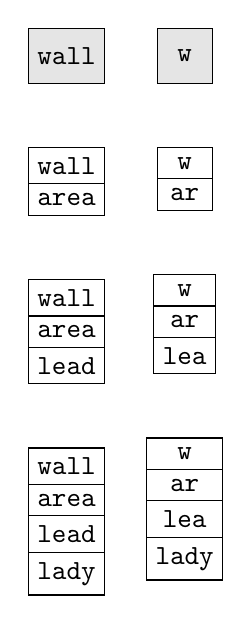
\begin{tikzpicture}
[my/.style={draw, rectangle, minimum size=7mm, fill=gray!20!}]
\node[my](0) at (0.5, 0) {\texttt{wall}};
\node[my](1) at (2.0, 0) {\texttt{w}};
\node[rectangle split,rectangle split parts=2,draw, text centered, minimum size=7mm](2) [below=8mm of 0] {\texttt{wall} \nodepart{second} \texttt{area}};
\node[rectangle split,rectangle split parts=2,draw, text centered, minimum size=7mm](3) [below=8mm of 1] {\texttt{w} \nodepart{second} \texttt{ar}};
\node[rectangle split,rectangle split parts=3,draw](4) [below=8mm of 2] {\texttt{wall} \nodepart{second} \texttt{area} \nodepart{third} \texttt{lead}};
\node[rectangle split,rectangle split parts=3,draw,text centered](5) [below=8mm of 3] {\texttt{w} \nodepart{second} \texttt{ar}\nodepart {third} \texttt{lea}};
\node[rectangle split,rectangle split parts=4,draw,text centered](6) [below=8mm of 4] {\texttt{wall} \nodepart{second} \texttt{area} \nodepart{third} \texttt{lead} \nodepart{fourth} \texttt{lady}};
\node[rectangle split,rectangle split parts=4,draw,text centered](7) [below=8mm of 5] {\texttt{w} \nodepart{second} \texttt{ar}\nodepart {third} \texttt{lea} \nodepart{fourth} \texttt{lady}};
\end{tikzpicture}
\end{center}
\end{figure}
\end{enumerate}
\end{itemize}

\setcounter{lstlisting}{0}
\begin{lstlisting}[style=customc, caption={Trie Tree}]

//trie struct definition
struct Trie
{
    vector<Trie*> m_next;
    //the index of the word contains the letter
    vector<size_t> m_index;

    Trie()
        : m_next( 26, nullptr )
    {}
};

vector<vector<string>> wordSquares( vector<string>& words )
{
    //build trie
    Trie* root = new Trie;
    for( size_t i = 0; i < words.size(); ++i )
    {
        build_trie( words[i], root, i );
    }

    //all words have same size
    int wl = static_cast<int>( words[0].size() );


    vector<vector<string>> ans;

    for( const auto& word : words )
    {
        //test each word
        //chec if a square can be built
        //buy put word in the first row
        vector<string> square( wl );

        square[0] = word;

        dfs( words, 1, square, ans, root );
    }

    return ans;
}

//W: the input word array
//start: the current column index
//M: the current word matrix
//ans: the result
//root: the root node of trie tree
void dfs( vector<string>& W, size_t start, vector<string>& M, vector<vector<string>>& ans, Trie* root )
{
    auto L = W[0].size();

    if( start == L )
    {
        //A word matrix is successfully built
        //add to result array
        ans.push_back( M );
        return;
    }

    //generate the prefix

    string prefix = "";

    for( size_t i = 0; i < start; ++i )
    {
        prefix += M[i][start];
    }

    //we will look for any word in W with this prefix
    //to put into the next row of word matrix
    auto node = root;

    for( auto c : prefix )
    {
        int ci = c - 'a';
        if( !node->m_next[ci] )
        {
            //no any word has this prefix
            return;
        }

        node = node->m_next[ci];
    }

    for( auto wi : node->m_index )
    {
        //W[wi] has the prefix
        //put it into row <start>
        M[start] = W[wi];
        //recursively build the matrix from <start+1>
        dfs( W, start + 1, M, ans, root );
    }
}


void build_trie( const string& w, Trie* root, size_t index )
{
    auto node  = root;

    for( auto c : w )
    {
        int ci = c - 'a';
        if( !node->m_next[ci] )
        {
            node->m_next[ci] = new Trie;
        }
        node = node->m_next[c - 'a'];
        //add current word index into the trie node
        node->m_index.push_back( index );
    }
}
\end{lstlisting}

\section{426 --- Convert Binary Search Tree to Sorted Doubly Linked List}
\textcolor{red}{Locked}
\\
Convert a BST to a sorted circular doubly-linked list in-place. Think of the left and right pointers as synonymous to the previous and next pointers in a doubly-linked list.
\par
Let's take the following BST as an example, it may help you understand the problem better:
\begin{figure}[H]
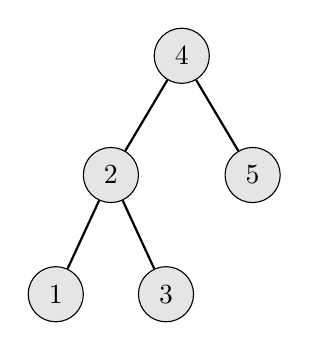
\begin{tikzpicture}
[my/.style={draw, circle, fill=gray!20!, minimum size=7mm}]
\node[my](0) at (0,0) {4};
\node[my](1) [below=8mm of 0, xshift=-9mm] {2};
\node[my](2) [below=8mm of 0, xshift=9mm] {5};
\node[my](3) [below=8mm of 1, xshift=-7mm] {1};
\node[my](4) [below=8mm of 1, xshift=7mm] {3};
\draw[thick] (0) -- (1); 
\draw[thick] (0) -- (2);
\draw[thick] (1) -- (3);
\draw[thick] (1) -- (4);
\end{tikzpicture}
\end{figure}

We want to transform this BST into a \textbf{circular doubly linked list}. Each node in a doubly linked list has a \textbf{predecessor} and \textbf{successor}. For a circular doubly linked list, the \textbf{predecessor} of the first element is the last element, and the \textbf{successor} of the last element is the first element.
\par
The figure below shows the circular doubly linked list for the BST above. The \texttt{head} symbol means the node it points to is the smallest element of the linked list.
 
\begin{figure}[H]
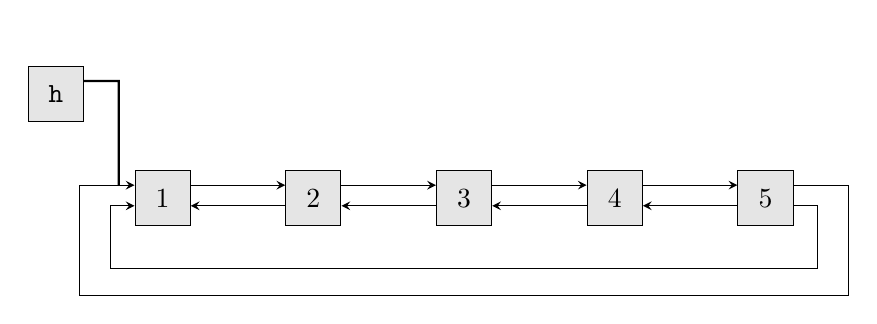
\begin{tikzpicture}
[my/.style={draw, rectangle, fill=gray!20!, minimum size=7mm}]
\node[my](0) at (0,0) {1};
\node[my](1) [right=12mm of 0] {2};
\draw[>=stealth,->] (0.25) -- (1.155);
\draw[>=stealth,->] (1.195) -- (0.345);
\node[my](2) [right=12mm of 1] {3};
\draw[>=stealth,->] (1.25) -- (2.155);
\draw[>=stealth,->] (2.195) -- (1.345);
\node[my](3) [right=12mm of 2] {4};
\draw[>=stealth,->] (2.25) -- (3.155);
\draw[>=stealth,->] (3.195) -- (2.345);
\node[my](4) [right=12mm of 3] {5};
\draw[>=stealth,->] (3.25) -- (4.155);
\draw[>=stealth,->] (4.195) -- (3.345);
\draw[>=stealth,->] (4.345) --  ++(3mm, 0) -- ++(0, -8mm) -| ($(0.195) - (3mm, 0)$) -- ++(3mm, 0);
\draw[>=stealth,->] (4.25) --  ++(7mm, 0) -- ++(0, -14mm) -| ($(0.155) - (7mm, 0)$) -- ++(7mm, 0);
\node[my](h) [above=8mm of 0.155, xshift=-10mm] {\texttt{h}};
%get the intersection of two paths
\path[name path=P1] ($(0.155)-(2mm, 0)$) -- ++(0, 20mm);
\path[name path=P2] (h.25) -- ++(20mm, 0);
\path[name intersections={of=P1 and P2, by={P0}}];
%\path [name intersections={of=P1 and P2,by={CS}}];
\draw[thick] (h.25) -- (P0) -- ($(0.155)-(2mm, 0)$);
\end{tikzpicture}
\end{figure}
Specifically, we want to do the transformation in place. After the transformation, the left pointer of the tree node should point to its predecessor, and the right pointer should point to its successor. We should return the pointer to the first element of the linked list.

The figure below shows the transformed BST. The solid line indicates the successor relationship, while the dashed line means the predecessor relationship.

\begin{figure}[H]
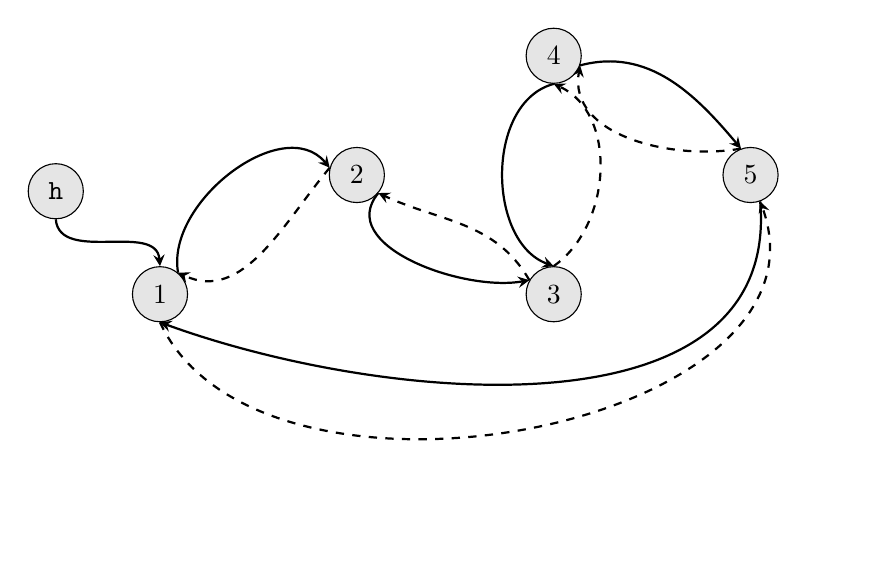
\begin{tikzpicture}
[my/.style={draw, circle, fill=gray!20!, minimum size=7mm}]
\node[my](0) at (0,0) {4};
\node[my](1) [below=8mm of 0, xshift=-25mm] {2};
\node[my](2) [below=8mm of 0, xshift=25mm] {5};
\node[my](3) [below=8mm of 1, xshift=-25mm] {1};
\node[my](4) [below=8mm of 1, xshift=25mm] {3};
\draw[thick, >=stealth,->] (0.south) to [out=195, in=160] (4.north);
\draw[dashed, thick, >=stealth,->] (4.north) to [out=35, in=335] (0.south);
\draw[thick, >=stealth,->] (0.340) to [out=15, in=130] (2.110);
\draw[dashed, thick, >=stealth,->] (2.110) to [out=190, in=260] (0.340);
\draw[thick, >=stealth,->] (1.320) to [out=230, in=190] (4.150);
\draw[dashed, thick, >=stealth,->] (4.150) to [out=120, in=335] (1.320);
%1--2
\draw[thick, >=stealth,->] (3.50) to [out=100, in=130] (1.165);
\draw[dashed, thick, >=stealth,->] (1.165) to [out=230, in=335] (3.50);
%1--5
\draw[thick, >=stealth,->] (2.290) to [out=275, in=340] (3.south);
\draw[dashed, thick, >=stealth,->] (3.south) to [out=295, in=290] (2.290);
%head
\node[my](h) [above=8mm of 3.155, xshift=-10mm] {\texttt{h}};
\draw[thick, >=stealth,->] (h.south) to [out=275, in=95] (3.north);
\end{tikzpicture}
\end{figure}

\subsection{Inorder Traverse}
\begin{itemize}
\item The inorder function need to update previous node and head node.
\item If we found the head node is null, this is the first time we get to a node. Update head and previous node to current node.
\item Otherwise, we connect previous node and current node with left and right pointers.
\item Finally, we connect the last node and head node with left and right pointers, then return head node.
\end{itemize}

\setcounter{lstlisting}{0}
\begin{lstlisting}[style=customc, caption={Inorder Traverse}]
/*
class Node
{
public:
    int val;
    Node* left;
    Node* right;

    Node() {}

    Node( int _val, Node* _left, Node* _right )
    {
        val = _val;
        left = _left;
        right = _right;
    }
}
*/
Node* treeToDoublyList( Node* root )
{
    if( !root )
    {
        return nullptr;
    }

    Node* head = nullptr;
    Node* pre = nullptr;

    inorder( root, head, pre );

    //connect the head node and the end node
    head->left = pre;
    pre->right = head;

    return head;
}

void inorder( Node* node, Node*& head, Node*& pre )
{
    if( !node )
    {
        return;
    }

    inorder( node->left, head, pre );

    if( !head )
    {
        //This is the first time
        //to access a node
        //this will be head node of the linked list
        head = node;
        pre = node;
    }
    else
    {
        //connect pre and node by
        //left and right pointers.
        pre->right = node;
        node->left = pre;
        pre = node;
    }

    inorder( node->right, head, pre );
}


\end{lstlisting}
\section{427 --- Construct Quad Tree}
We want to use quad trees to store an $N \times N$ boolean grid. Each cell in the grid can only be \texttt{true} or \texttt{false}. The root node represents the whole grid. For each node, it will be subdivided into four children nodes \textbf{until the values in the region it represents are all the same}.

Each node has another two boolean attributes : \texttt{isLeaf} and \texttt{val}. \texttt{isLeaf} is \texttt{true} if and only if the node is a leaf node. The \texttt{val} attribute for a leaf node contains the value of the region it represents.

Your task is to use a quad tree to represent a given grid. The following example may help you understand the problem better:

Given the 8 x 8 grid below, we want to construct the corresponding quad tree:


\subsection{Depth First Search From Top To Bottom}
\begin{itemize}
\item In this method, each time, we check if the large grid has one uniform value or not. If it is, we create a leaf node to represent this grid.
\item Otherwise, we split the grid into four parts and recursively apply the same process.
\item To speed up the checking, we may use 2D prefix sum of the grid.
\end{itemize}

\setcounter{lstlisting}{0}
\begin{lstlisting}[style=customc, caption={Build From Top To Bottom}]
Node* construct( vector<vector<int>>& grid )
{
    int N = static_cast<int>( grid.size() );

    vector<vector<int>> g_sum( N + 1, vector<int>( N + 1, 0 ) );

    //build 2d prefix sum
    //for input grid
    for( int r = 0;  r < N; ++r )
    {
        for( int c = 0; c < N; ++c )
        {
            g_sum[r + 1][c + 1] = g_sum[r + 1][c] + g_sum[r][c + 1] - g_sum[r][c] + grid[r][c];
        }
    }

    //run top to bottom build
    return dfs( grid, 0, 0, N - 1, N - 1, g_sum );
}

Node* dfs( vector<vector<int>>&grid, int top, int left, int bottom, int right, vector<vector<int>>& g_sum )
{
    if( ( top > bottom ) || ( left > right ) )
    {
        //base case
        return nullptr;
    }

    //get the sum of grid[top...bottom][left...right]
    int sum = g_sum[bottom + 1][right + 1] -
              g_sum[top][right + 1] -
              g_sum[bottom + 1][left]
              + g_sum[top][left];

    //the whole sum if grid[top...bottom][left...right] all are 1s or 0s
    int area = ( bottom - top + 1 ) * ( right - left + 1 ) * grid[top][left];

    if( sum == area )
    {
        //grid[top...bottom][left...right]
        //are all same values
        //it forms a leaf node
        Node* node = new Node;
        //must set all 4 nodes
        //to nullptr, otherwise will
        //cause exception
        node->topLeft = nullptr;
        node->topRight = nullptr;
        node->bottomLeft = nullptr;
        node->bottomRight = nullptr;

        node->val = grid[top][left] ? true : false;
        node->isLeaf = true;

        return node;
    }

    //divide grid[top...bottom][left...right] into 4 parts
    //from the middle of row and column
    int mid_r = ( top + bottom ) / 2;
    int mid_c = ( left + right ) / 2;

    Node* node = new Node;
    node->topLeft = dfs( grid, top, left, mid_r, mid_c, g_sum );
    node->topRight = dfs( grid, top, mid_c + 1, mid_r, right, g_sum );
    node->bottomLeft = dfs( grid, mid_r + 1, left, bottom, mid_c, g_sum );
    node->bottomRight = dfs( grid, mid_r + 1, mid_c + 1, bottom, right, g_sum );

    node->isLeaf = false;
    //must set node->val = false
    //otherwise, it will cause exception
    node->val = false;

    return node;
}
\end{lstlisting}

\subsection{Depth First Search From Bottom To Top}
\begin{itemize}
\item We can build from each element of the grid.
\item Then, we combine 4 connected nodes.
\item If the four nodes are all leaves and same values, we can combine them into one leaf node and delete these 4 nodes.
\item Otherwise, create a node to contains these 4 nodes.
\item Recursively apply the above process to the input grid.
\end{itemize}

\begin{lstlisting}[style=customc, caption={Build From Bottom To Top}]
Node* construct( vector<vector<int>>& grid )
{
    int N = static_cast<int>( grid.size() );
    return dfs( grid, 0, 0, N );
}

Node* dfs( vector<vector<int>>&grid, int x, int y, int size )
{
    if( size == 1 )
    {
        //this is each element in the grid
        return new Node{grid[x][y] == 1, true, nullptr, nullptr, nullptr, nullptr};
    }

    auto tl = dfs( grid, x, y, size / 2 );
    auto tr = dfs( grid, x, y + size / 2, size / 2 );
    auto bl = dfs( grid, x + size / 2, y, size / 2 );
    auto br = dfs( grid, x + size / 2, y + size / 2, size / 2 );

    if( ( tl->isLeaf && tr->isLeaf && bl->isLeaf && br->isLeaf ) )
    {
        if( ( tl->val == tr->val ) && ( bl->val == br->val ) && ( tl->val == bl->val ) )
        {
            //we can merge these 4 nodes
            //into one leaf node
            auto node = new Node;
            node->isLeaf = true;
            node->val = tl->val;

            node->topLeft = nullptr;
            node->topRight = nullptr;
            node->bottomLeft = nullptr;
            node->bottomRight = nullptr;

            //delete these nodes
            delete tl;
            delete tr;
            delete bl;
            delete br;

            return node;
        }
    }

    //create a new node to contain these 4 nodes
    return new Node{false, false, tl, tr, bl, br};
}
\end{lstlisting}
\section{428 --- Serialize and Deserialize N-ary Tree}
\textcolor{red}{Locked}
\\
Serialization is the process of converting a data structure or object into a sequence of bits so that it can be stored in a file or memory buffer, or transmitted across a network connection link to be reconstructed later in the same or another computer environment.
\par
Design an algorithm to \textbf{serialize} and \textbf{deserialize} an $N$-ary tree. An $N$-ary tree is a rooted tree in which each node has no more than $N$ children. There is no restriction on how your \textbf{serialization}/\textbf{deserialization} algorithm should work. You just need to ensure that an $ N $-ary tree can be serialized to a string and this string can be deserialized to the original tree structure.

For example, you may serialize the following 3-ary tree

\begin{figure}[H]
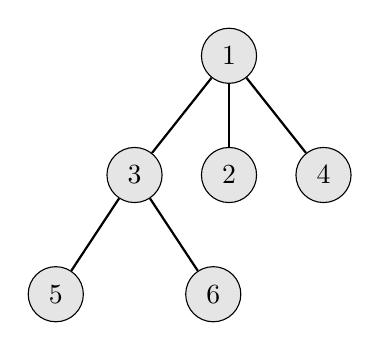
\begin{tikzpicture}
[my/.style={draw, circle, minimum size=7mm, fill=gray!20!}]
\node[my](0) at (0,0) {1};
\node[my](1) [below=8mm of 0, xshift=-12mm] {3};
\node[my](2) [below=8mm of 0] {2};
\node[my](3) [below=8mm of 0, xshift=12mm] {4};
\node[my](4) [below=8mm of 1, xshift=-10mm] {5};
\node[my](5) [below=8mm of 1, xshift=10mm] {6};
\draw[thick] (0)--(1)--(4);
\draw[thick] (1)--(5);
\draw[thick] (0)--(2);
\draw[thick] (0)--(3);
\end{tikzpicture}
\end{figure}
as [1 [3[5 6] 2 4]]. You do not necessarily need to follow this format, so please be creative and come up with different approaches yourself.

\paragraph{Note:}
\begin{itemize}
\item $ N $ is in the range of $[1, 1000]$
\item Do not use class member/global/static variables to store states. Your serialize and deserialize algorithms should be stateless.
\end{itemize}

\subsection{Preorder Traverse}
\begin{itemize}
\item Serialize: 
\begin{enumerate}
\item Fo a null node, add a special character like \#
\item Otherwise, add the node's value first, then add a space, and then the number of its children, and then add a space again.
\item If it has children, recursively traverse into each child node, do the above operation again.
\end{enumerate}
\item Deserialize: We may need \texttt{istringstream} to help read the string as a input stream.
\begin{enumerate}
\item Read the value from the stream. If the special character is the value, return the null node.
\item Otherwise, read the number of children from the stream. 
\item Create a new node with read value.
\item By the number of children, we add a recursively-built node into the children array of current node.
\item Finally, return the current node
\end{enumerate}
\end{itemize}

\setcounter{lstlisting}{0}
\begin{lstlisting}[style=customc, caption={Recursion}]
/*
class Node
{
public:
    int val;
    vector<Node*> children;

    Node()
    {}
}
*/
// Encodes a tree to a single string.
string serialize( Node* root )
{
    string tree;
    preorder( root, tree );
    return tree;
}

void preorder( Node* node, string& stree )
{
    if( !node )
    {
        stree.push_back( '#' );
    }

    //val + space + number of children + space
    stree += to_string( node->val );
    stree.push_back( ' ' );

    if( node->children.empty() )
    {
        stree.push_back( '0' );
        stree.push_back( ' ' );
    }
    else
    {
        stree += to_string( node->children.size() );
        stree.push_back( ' ' );

        for( auto child : node->children )
        {
            //recursively serialize the child
            preorder( child, stree );
        }
    }

    return;

}

// Decodes your encoded data to tree.
Node* deserialize( string data )
{
    std::istringstream iss( data );
    return build( iss );
}

Node* build( std::istringstream& iss )
{
    string sval;
    string slen;

    //read value first
    iss >> sval;

    if( sval[0] == '#' )
    {
        return nullptr;
    }

    //read lenth then
    iss >> slen;

    int val = stoi( sval );

    //create the new node
    Node* node = new Node();
    node->val = val;

    int len = stoi( slen );

    if( len > 0 )
    {
        for( int i = 0; i < len; ++i )
        {
            //recursively build child
            //add child into node->children
            node->children.push_back( build( iss ) );
        }
    }
    return node;
}
\end{lstlisting}

\section{429 --- N-ary Tree Level Order Traversal}
Given an $n$-ary tree, return the level order traversal of its nodes' values. (ie, from left to right, level by level).

For example, given a 3-ary tree:

\begin{figure}[H]
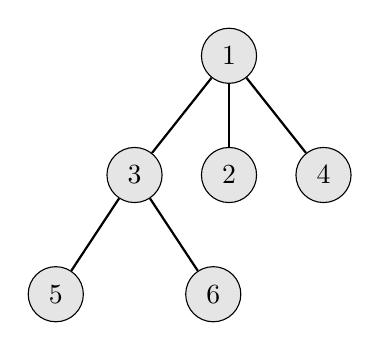
\begin{tikzpicture}
[my/.style={draw, circle, minimum size=7mm, fill=gray!20!}]
\node[my](0) at (0,0) {1};
\node[my](1) [below=8mm of 0, xshift=-12mm] {3};
\node[my](2) [below=8mm of 0] {2};
\node[my](3) [below=8mm of 0, xshift=12mm] {4};
\node[my](4) [below=8mm of 1, xshift=-10mm] {5};
\node[my](5) [below=8mm of 1, xshift=10mm] {6};
\draw[thick] (0)--(1)--(4);
\draw[thick] (1)--(5);
\draw[thick] (0)--(2);
\draw[thick] (0)--(3);
\end{tikzpicture}
\end{figure}

We should return its level order traversal:
\begin{table}[H]
\begin{tabular}{lll}
1 & & \\
3 & 2 & 4\\
5 & 6 & 
\end{tabular}
\end{table}

\paragraph{Note:}

\begin{itemize}
\item The depth of the tree is at most 1000.
\item The total number of nodes is at most 5000.
\end{itemize}

\subsection{Queue}
典型的运用queue进行层次遍历的例子。

\setcounter{lstlisting}{0}
\begin{lstlisting}[style=customc, caption={Queue}]
vector<vector<int>> levelOrder( Node* root )
{
    if( !root )
    {
        return {};
    }

    queue<Node*> q;

    q.push( root );

    vector<vector<int>> ans;

    while( !q.empty() )
    {
        auto sz = q.size();

        //current level data
        vector<int> level;

        for( size_t i = 0; i < sz; ++i )
        {

            auto node = q.front();
            q.pop();

            level.push_back( node->val );

            for( auto child :  node->children )
            {
                if( child )
                {
                    q.push( child );
                }
            }
        }

        ans.push_back( move( level ) );
    }

    return ans;
}
\end{lstlisting}

\section{430 --- Flatten a Multilevel Doubly Linked List}
You are given a doubly linked list which in addition to the next and previous pointers, it could have a child pointer, which may or may not point to a separate doubly linked list. These child lists may have one or more children of their own, a nd so on, to produce a multilevel data structure, as shown in the example below.

\begin{figure}[H]
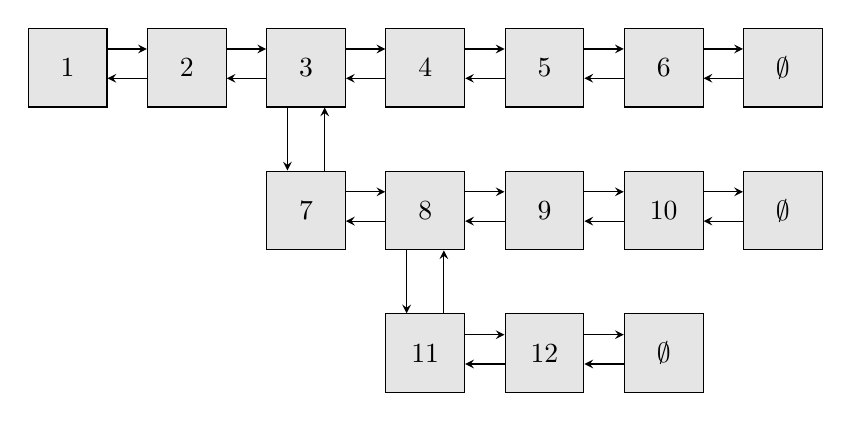
\begin{tikzpicture}
[my/.style={draw, rectangle, minimum size = 1cm, fill=gray!20!},
node distance=8mm and 5mm, >=stealth,->]
\node[my](0) at (0,0) {1};
\node[my](1) [right=of 0] {2};
\node[my](2) [right=of 1] {3};
\node[my](3) [right=of 2] {4};
\node[my](4) [right=of 3] {5};
\node[my](5) [right=of 4] {6};
\node[my](6) [right=of 5] {$\emptyset$};
\draw (0.25) -- (1.155);
\draw (1.195) -- (0.345);
\draw (1.25) -- (2.155);
\draw (2.195) -- (1.345);
\draw (2.25) -- (3.155);
\draw (3.195) -- (2.345);
\draw (3.25) -- (4.155);
\draw (4.195) -- (3.345);
\draw (4.25) -- (5.155);
\draw (5.195) -- (4.345);
\draw (5.25) -- (6.155);
\draw (6.195) -- (5.345);
%level2
\node[my](7) [below=of 2] {7};
\node[my](8) [right=of 7] {8};
\node[my](9) [right=of 8] {9};
\node[my](10) [right=of 9] {10};
\node[my](e1) [right=of 10] {$\emptyset$};
\draw (2.245) -- (7.115);
\draw (7.65) -- (2.295);
\draw (7.25) -- (8.155);
\draw (8.195) -- (7.345);
\draw (8.25) -- (9.155);
\draw (9.195) -- (8.345);
\draw (9.25) -- (10.155);
\draw (10.195) -- (9.345);
\draw (10.25) -- (e1.155);
\draw (e1.195) -- (10.345);
%level 3
\node[my](11) [below=of 8] {11};
\node[my](12) [right=of 11] {12};
\node[my](e2) [right=of 12] {$\emptyset$};
\draw (8.245) -- (11.115);
\draw (11.65) -- (8.295);
\draw (11.25) -- (12.155);
\draw (12.195) -- (11.345);
\draw (12.25) -- (e2.155);
\draw (e2.195) -- (12.345);
\end{tikzpicture}
\end{figure}

Flatten the list so that all the nodes appear in a single-level, doubly linked list. You are given the head of the first level of the list.

\begin{figure}[H]
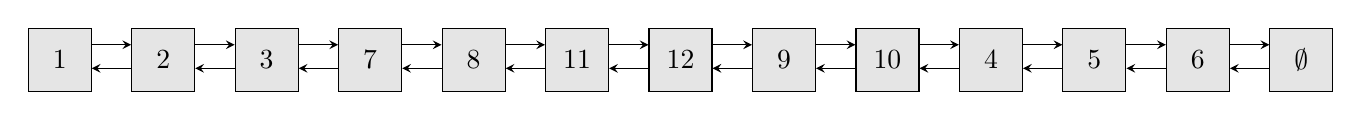
\begin{tikzpicture}
[my/.style={draw, rectangle, minimum size = 8mm, fill=gray!20!},
node distance=5mm, >=stealth,->]
\node[my](0) at (0,0) {1};
\node[my](1) [right=of 0] {2};
\node[my](2) [right=of 1] {3};

\node[my](7) [right=of 2] {7};
\node[my](8) [right=of 7] {8};


\node[my](11) [right=of 8] {11};
\node[my](12) [right=of 11] {12};

\node[my](9) [right=of 12] {9};
\node[my](10) [right=of 9] {10};

\node[my](3) [right=of 10] {4};
\node[my](4) [right=of 3] {5};
\node[my](5) [right=of 4] {6};
\node[my](e) [right=of 5] {$\emptyset$};

\draw (0.25) -- (1.155);
\draw (1.195) -- (0.345);
\draw (1.25) -- (2.155);
\draw (2.195) -- (1.345);

\draw (2.25) -- (7.155);
\draw (7.195) -- (2.345);


\draw (7.25) -- (8.155);
\draw (8.195) -- (7.345);

\draw (8.25) -- (11.155);
\draw (11.195) -- (8.345);


\draw (11.25) -- (12.155);
\draw (12.195) -- (11.345);

\draw (12.25) -- (9.155);
\draw (9.195) -- (12.345);

\draw (9.25) -- (10.155);
\draw (10.195) -- (9.345);

\draw (10.25) -- (3.155);
\draw (3.195) -- (10.345);


\draw (3.25) -- (4.155);
\draw (4.195) -- (3.345);
\draw (4.25) -- (5.155);
\draw (5.195) -- (4.345);

\draw (5.25) -- (e.155);
\draw (e.195) -- (5.345);


\end{tikzpicture}
\end{figure}

\subsection{Flatter One Level Each Time}
\begin{itemize}
\item Iterate over the list. If current node has a child, we iterate over from the child until the last node of the child list.
\item Connect the pointer of the last node with current node's next node.
\item Connect the pointer of current node and it child.
\item Set current node's child as null.
\item Go to the next node of current node.
\item In this way, we flatten one child list at a time. Even though the child list may contain another grandchild list, we iterate from current node's next which will iterate over the child list again.
\end{itemize}

\setcounter{lstlisting}{0}
\begin{lstlisting}[style=customc, caption={Flatten one list at a time}]
/*
// Definition for a Node.
class Node {
public:
    int val;
    Node* prev;
    Node* next;
    Node* child;

    Node() {}

    Node(int _val, Node* _prev, Node* _next, Node* _child) {
        val = _val;
        prev = _prev;
        next = _next;
        child = _child;
    }
};
*/

Node* flatten( Node* head )
{
    auto node = head;
    while( node )
    {
        if( node->child )
        {
            auto next = node->next;

            //connect prev and next pointers of node and its child
            node->child->prev = node;
            node->next = node->child;
            node->child = nullptr;

            //iterate over the child list
            auto x = node->next;

            //search the last node
            while( x->next )
            {
                x = x->next;
            }

            //connect prev and next pointers of x and next node
            x->next = next;
            if( next )
            {
                next->prev = x;
            }
        }

        //forward to the next node
        //we may iterate over the child list again
        node = node->next;
    }
    return head;
}
\end{lstlisting}
%\section{431 --- Encode N-ary Tree to Binary Tree}
Design an algorithm to encode an $N$-ary tree into a binary tree and decode the binary tree to get the original $N$-ary tree. An $N$-ary tree is a rooted tree in which each node has no more than $ N $ children. Similarly, a binary tree is a rooted tree in which each node has no more than 2 children. There is no restriction on how your encode/decode algorithm should work. You just need to ensure that an $ N $-ary tree can be encoded to a binary tree and this binary tree can be decoded to the original N-nary tree structure.

For example, you may encode the following 3-ary tree to a binary tree in this way:

\begin{figure}[H]
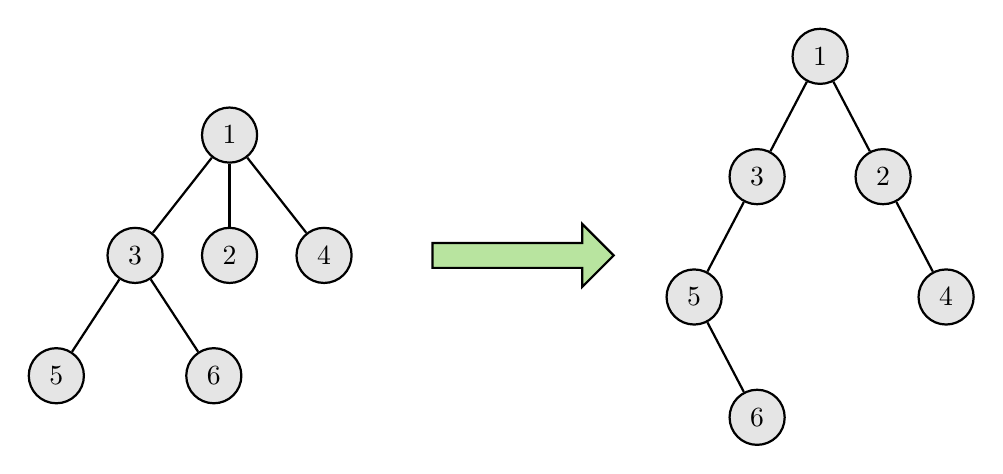
\begin{tikzpicture}
[my/.style={draw, circle, minimum size=7mm, fill=gray!20!}, thick]
\node[my](0) at (0,0) {1};
\node[my](1) [below=8mm of 0, xshift=-12mm] {3};
\node[my](2) [below=8mm of 0] {2};
\node[my](3) [below=8mm of 0, xshift=12mm] {4};
\node[my](4) [below=8mm of 1, xshift=-10mm] {5};
\node[my](5) [below=8mm of 1, xshift=10mm] {6};
\draw (0)--(1)--(4);
\draw (1)--(5);
\draw (0)--(2);
\draw (0)--(3);

\node[draw, single arrow, minimum height=23mm, minimum width=8mm, single arrow head extend=2mm, anchor=west, fill=yellow!30!green!40!] at ($(3.east) + (1cm, 0)$) {};

\node[my] (11) at (7.5, 1) {1};
\node[my] (21) [below=8mm of 11, xshift=-8mm] {3};
\node[my] (31) [below=8mm of 11, xshift=8mm] {2};
\node[my] (41) [below=8mm of 21, xshift=-8mm] {5};
\node[my] (51) [below=8mm of 31, xshift=8mm] {4};
\node[my] (61) [below=8mm of 41, xshift=8mm] {6};
\draw (11)--(21);
\draw (11)--(31);
\draw (31)--(51);
\draw (21)--(41);
\draw (41)--(61);
\end{tikzpicture}
\end{figure}


Note that the above is just an example which might or might not work. You do not necessarily need to follow this format, so please be creative and come up with different approaches yourself.

\paragraph{Note:}

\begin{itemize}
\item $ N $ is in the range of [1, 1000]
\item Do not use class member/global/static variables to store states. Your encode and decode algorithms should be stateless.
\end{itemize}

\subsection{One Possible Approach}
\begin{itemize}
\item In encoding, put the first child as the left child, and each sibling becomes its previous one's right child.
\item In decoding, get the left child as the first child, and add its right decedents as its siblings. 
\end{itemize}

\setcounter{lstlisting}{0}
\begin{lstlisting}[style=customc, caption={Left Child And Right Decendents}]
class Codec
{
public:
    // Encodes an n-ary tree to a binary tree.
    TreeNode* encode( Node* root )
    {
        if( !root )
        {
            return nullptr;
        }

        TreeNode* t_node = new TreeNode( root->val );
        if( !root->children.empty() )
        {
            //set the first child as the left child
            //since the first child may contain other node
            //we recursively build the child tree
            //with root as root->children[0]
            t_node->left = encode( root->children[0] );
            auto t = t_node->left;

            //set the siblings as the right decendents
            //of left child
            for( size_t i = 1; i < root->children.size(); ++i )
            {
                //recursively build the child tree
                //with root as root->children[i]
                t->right = encode( root->children[i] );
                t = t->right;
            }
        }

        return t_node;
    }

    // Decodes your binary tree to an n-ary tree.
    Node* decode( TreeNode* root )
    {
        if( !root )
        {
            return nullptr;
        }

        Node* node = new Node;
        node->val = root->val;

        if( root->left )
        {
            //first child
            //recursively process current root->left
            node->children.push_back( decode( root->left ) );

            auto t_node = root->left->right;

            //add right decendents
            //as the siblings
            while( t_node )
            {
                //recursively process current node
                node->children.push_back( decode( t_node ) );
                t_node = t_node->right;
            }
        }

        return node;
    }
};
 \end{lstlisting}
%\section{432 --- All O`one Data Structure}
Implement a data structure supporting the following operations:


\begin{lstlisting}[style=customc]
/*
Inserts a new key with value 1. 
Or increments an existing key by 1. 
Key is guaranteed to be a non-empty string.
*/
Inc(Key) 

/*
If Key's value is 1, remove it from the data structure. 
Otherwise decrements an existing key by 1. 
If the key does not exist,this function does nothing. 
Key is guaranteed to be a non-empty string.
*/
Dec(Key)

/*
Returns one of the keys with maximal value. 
If no element exists, return an empty string.
*/

GetMaxKey()

/*
Returns one of the keys with minimal value. 
If no element exists, return an empty string
*/
GetMinKey()
\end{lstlisting}

\paragraph{Challenge:} 
\begin{itemize}
\item Perform all these in $O(1)$ time complexity.
\end{itemize}

\subsection{Hash Map With Double Linked List}
\begin{itemize}
\item We use a struct \texttt{Bucket} to store the value and the associated keys.
\item Store the buckets in a double linked list, $L$, and associate the key with the position of its bucket in the list through a hash map, $M$.
\item We put the bucket with the least value at the end of the list, and the bucket with largest value in the front.
\item When the value of the key is changed, we have to check their previous or successive bucket to see if the value inside is either 1 greater or 1 smaller than current value of the key. If not, we have to create a new bucket to store the new value and the key. Also, remove the key from it's current bucket and change the hash map when possible.
\end{itemize}


\setcounter{lstlisting}{0}
\begin{lstlisting}[style=customc, caption={Double Linked List and Iterator For Value In Hash Map}]
class AllOne
{
public:
    /** Initialize your data structure here. */
    AllOne()
    {

    }

    /** Inserts a new key <Key> with value 1. Or increments an existing key by 1. */
    void inc( string key )
    {
        auto it = m_dict.find( key );
        if( it == m_dict.end() )
        {
            //new key
            //since value 1 is the smallest value
            //we put this at the back of the list
            if( m_bl.empty() || ( m_bl.back().val != 1 ) )
            {
                m_bl.push_back( {1, unordered_set<string>{key}} );
            }
            else
            {
                m_bl.back().keys.insert( key );
            }

            //add the position of the bucket
            //that containing the new key
            //to the hash map
            auto p_bl = m_bl.end();
            --p_bl;

            m_dict.emplace( key, p_bl );
        }
        else
        {
            //we already have this key
            //we must increments its existing value
            //since the value is changed
            //it must be placed into another or new bucket

            auto p_bl = it->second;

            //check the previous bucekt
            auto prev = p_bl;
            if( prev != m_bl.begin() )
            {
                --prev;
            }

            if( prev->val != p_bl->val + 1 )
            {
                //since the previous bucket
                //contains a value larger than
                //p_bl->val + 1,
                //we must create a new bucket before p_bl to
                //store the new value and its related string
                auto new_p = m_bl.insert( p_bl, {p_bl->val + 1, unordered_set<string>{key}} );

                //we also have to change the dictionary
                it->second = new_p;
            }
            else
            {
                //this bucket will contain this new key
                prev->keys.insert( key );

                //we also have to change the dictionary
                it->second = prev;
            }

            //in either case
            //we have to remove this key from current bucket
            p_bl->keys.erase( key );

            if( p_bl->keys.empty() )
            {
                //no key inside this bucket
                //remove it from the list
                m_bl.erase( p_bl );
            }
        }//end else
    }

    /** Decrements an existing key by 1. If Key's value is 1, remove it from the data structure. */
    void dec( string key )
    {
        auto it = m_dict.find( key );
        if( it == m_dict.end() )
        {
            return;
        }

        auto p_bl = it->second;

        if( p_bl->val == 1 )
        {
            //remove the key from the bucket
            p_bl->keys.erase( key );

            p_bl->keys.erase( key );
            if( p_bl->keys.empty() )
            {
                //no key inside this bucket
                //remove it from the list
                m_bl.erase( p_bl );
            }

            //remove the key from the dictionary
            m_dict.erase( key );
            return;
        }

        //the value of the key decrements
        //we have to check if the next one of this bucket
        //has the same value as the key
        auto next_p = p_bl;
        ++next_p;
        if( ( next_p == m_bl.end() ) || ( next_p->val != p_bl->val - 1 ) )
        {
            //we have to create a new bucket before next_p to
            //contain this new value
            auto new_p = m_bl.insert( next_p, {p_bl->val - 1, unordered_set<string>{key}} );
            //we also have to change the dictionary
            it->second = new_p;
        }
        else
        {
            //we add the key to the bucket in next_p
            next_p->keys.insert( key );

            //we also have to change the dictionary
            it->second = next_p;
        }

        //in either case, we have to remove key from
        //the bucket in p_bl
        p_bl->keys.erase( key );
        if( p_bl->keys.empty() )
        {
            //no key inside this bucket
            //remove it from the list
            m_bl.erase( p_bl );
        }
    }

    /** Returns one of the keys with maximal value. */
    string getMaxKey()
    {
        if( m_bl.empty() )
        {
            return "";
        }

        //max value is the front of the list
        auto b = m_bl.front().keys.begin();
        return *b;
    }

    /** Returns one of the keys with Minimal value. */
    string getMinKey()
    {
        if( m_bl.empty() )
        {
            return "";
        }

        //min value is the back of the list
        auto b = m_bl.back().keys.begin();
        return *b;
    }

private:

    struct Bucket
    {
        int val = -1;
        unordered_set<string> keys;

        Bucket() = default;
    };

    list<Bucket> m_bl;

    unordered_map<string, list<Bucket>::iterator> m_dict;
};
\end{lstlisting}
%\section{433 --- Minimum Genetic Mutation}
A gene string $S$ can be represented by an 8-character long string, with choices from \texttt{A}, \texttt{C}, \texttt{G}, \texttt{T}.

Suppose we need to investigate about a mutation (mutation from start to end), where \texttt{ONE} mutation is defined as \texttt{ONE} single character changed in the gene string.

For example, \texttt{AACCGGTT} $\longrightarrow$ \texttt{AACCGGTA} is 1 mutation.

Also, there is a given gene bank, which records all the valid gene mutations. A gene must be in the bank to make it a valid gene string.

Now, given 3 things - start $s$, end $t$, bank $B$, your task is to determine what is the minimum number of mutations needed to mutate from start to end. If there is no such a mutation, return $-1$.

\paragraph{Note:}

\begin{itemize}
\item Starting point is assumed to be valid, so it might not be included in the bank.
\item If multiple mutations are needed, all mutations during in the sequence must be valid.
\item You may assume start and end string is not the same.
\end{itemize}
 

\paragraph{Example 1:}

\begin{flushleft}
\textbf{Input}: $s$: \texttt{AACCGGTT}, $e$: \texttt{AACCGGTA}, $B$: [\texttt{AACCGGTA}]
\\
\textbf{Output}: 1
\end{flushleft}
 

\paragraph{Example 2:}
\begin{flushleft}
\textbf{Input}: $s$: \texttt{AACCGGTT}, $e$: \texttt{AACCGGTA}, $B$: [\texttt{AACCGGTA}, \texttt{AACCGCTA}, \texttt{AAACGGTA}]
\\
\textbf{Output}: 2
\end{flushleft} 


\paragraph{Example 3:}
\begin{flushleft}
\textbf{Input}: $s$: \texttt{AAAAACCC}, $e$: \texttt{AACCCCCC}, $B$: [\texttt{AAAACCCC}, \texttt{AAACCCCC}, \texttt{AACCCCCC}]
\\
\textbf{Output}: 3
\end{flushleft} 

\subsection{Two-way Breadth First Search}

\setcounter{lstlisting}{0}
\begin{lstlisting}[style=customc, caption={Two-way Breadth First Search}]
int minMutation( string start, string end, vector<string>& bank )
{
    //change to hash set
    unordered_set<string> z( bank.begin(), bank.end() );

    //the target string is not in the bank
    if( z.find( end ) == z.end() )
    {
        return -1;
    }

    //forward: from start to end
    unordered_set<string> f;
    f.emplace( start );

    //backward: from end to start
    unordered_set<string> b;
    b.emplace( end );

    //The level from start to end
    int f_level = 0;

    //The level from end to start
    int b_level = 0;

    char gens[4] = {'A', 'C', 'G', 'T'};

    //helper functon to get mutated strings from current gen strings
    auto next_level = [&z, &gens]( unordered_set<string>& cur, unordered_set<string>& next )
    {
        for( const auto& s : cur )
        {
            string m = s;
            for( size_t i = 0; i < s.size(); ++i )
            {

                for( char gen : gens )
                {
                    if( s[i] == gen ) continue;
                    m[i] = gen;

                    //the mutated string needs to be in the bank
                    //and does not show before
                    if( ( z.find( m ) != z.end() ) && ( cur.find( m ) == cur.end() ) )
                    {
                        next.emplace( m );
                    }

                    m[i] = s[i];
                }
            }
        }
    };

    while( !f.empty()  && !b.empty() )
    {
        unordered_set<string> f_next;

        next_level( f, f_next );

        ++f_level;

        //search the mutated strings of next level from forward direction
        //in backward level
        for( const auto& nf : f_next )
        {
            if( b.find( nf ) != b.end() )
            {
                return f_level + b_level;
            }
        }

        unordered_set<string> b_next;
        next_level( b, b_next );

        ++b_level;

        //search the mutated strings of next level from backward direction
        //in forward level

        for( const auto& nb : b_next )
        {
            if( f_next.find( nb ) != f_next.end() )
            {
                return f_level + b_level;
            }
        }

        //update f as next level
        swap( f, f_next );
        //update b as next level
        swap( b, b_next );
    }

    return -1;
}
\end{lstlisting}
%\section{434 --- Number of Segments in a String}
Count the number of segments in a string $s$, where a segment is defined to be a contiguous sequence of non-space characters.

Please note that the string does not contain any non-printable characters.

\paragraph{Example:}

\begin{flushleft}
\textbf{Input}: Hello, my name is John
\\
\textbf{Output}: 5
\end{flushleft}

\subsection{In-Place}

\setcounter{lstlisting}{0}
\begin{lstlisting}[style=customc, caption={In-place}]
int countSegments( string s )
{
    if( s.empty() )
    {
        return 0;
    }

    if( s.back() != ' ' )
    {
        s.push_back( ' ' );
    }

    //last indicates the last non-space
    //character before a new space
    size_t last = s.size();

    int ans = 0;

    for( size_t i = 0; i < s.size(); ++i )
    {
        if( s[i] == ' ' )
        {
            //to avoid repeat counting
            //make sure last is close to i
            if( last == i - 1 )
            {
                ++ans;
            }

            continue;
        }

        //update the position of last non-space character
        last = i;
    }

    return ans;
}
};
\end{lstlisting}
%\section{435 --- Non-overlapping Intervals}
Given a collection of intervals $I$, find the minimum number of intervals you need to remove to make the rest of the intervals non-overlapping.

\paragraph{Note:}

\begin{itemize}
\item You may assume the interval's end point is always bigger than its start point.
\item Intervals like [1,2] and [2,3] have borders \textbf{touching} but they don't overlap each other.
\end{itemize}
 

\paragraph{Example 1:}

\begin{flushleft}
\textbf{Input}: [ [1,2], [2,3], [3,4], [1,3] ]

\textbf{Output}: 1

\textbf{Explanation}: [1,3] can be removed and the rest of intervals are non-overlapping.
\end{flushleft}
 

\paragraph{Example 2:}

\begin{flushleft}
\textbf{Input}: [ [1,2], [1,2], [1,2] ]

\textbf{Output}: 2

\textbf{Explanation}: You need to remove two [1,2] to make the rest of intervals non-overlapping.
\end{flushleft}
 

\paragraph{Example 3:}

\begin{flushleft}
\textbf{Input}: [ [1,2], [2,3] ]

\textbf{Output}: 0

\textbf{Explanation}: You don't need to remove any of the intervals since they're already non-overlapping.
\end{flushleft}

\subsection{Count Non-Overlapped Intervals}
The following greedy algorithm does find a set of non-overlapping intervals of maximum size:

\begin{itemize}
\item Select the interval, $x$, with the earliest finishing time.
\item Remove $x$, and all intervals intersecting x, from the set of candidate intervals.
\item Repeat until the set of candidate intervals is empty.
\end{itemize}


\setcounter{lstlisting}{0}
\begin{lstlisting}[style=customc, caption={Count Maximum Non-overlapping Intervals}]
int eraseOverlapIntervals( vector<vector<int>>& intervals )
{
    if( intervals.empty() )
    {
        return 0;
    }

    //according to the greedy algorithm
    //we need sort the intervals per the end
    sort( intervals.begin(), intervals.end(), []( const vector<int>& v1, const vector<int>& v2 )
    {
        if( v1[1] < v2[1] )
        {
            return true;
        }
        else if( v1[1] == v2[1] )
        {
            return v1[0] < v2[0];
        }

        return false;
    } );

    //count is the number of non-overlapping intervals
    int count = 1;

    int last = intervals[0][1];

    for( size_t i = 1; i < intervals.size(); ++i )
    {
        if( intervals[i][0] >= last )
        {
            //only count the ones does not touch with last
            ++count;
            last = intervals[i][1];
        }
    }


    return static_cast<int>( intervals.size() ) - count;

}
\end{lstlisting}
%\section{436 --- Find Right Interval}
Given a set of intervals $I$, for each of the interval $i$, check if there exists an interval $j$ whose start point is bigger than or equal to the end point of the interval $i$, which can be called that $j$ is on the \texttt{right} of $ i $.

For any interval $ i $, you need to store the minimum interval $ j $'s index, which means that the interval $ j $ has the minimum start point to build the \texttt{right} relationship for interval $ i $. If the interval $ j $ doesn't exist, store $-1$ for the interval i. Finally, you need output the stored value of each interval as an array.

\paragraph{Note:}

\begin{itemize}
\item You may assume the interval's end point is always bigger than its start point.
\item You may assume none of these intervals have the same start point.
\end{itemize}
 

\paragraph{Example 1:}

\begin{flushleft}
\textbf{Input}: [ [1,2] ]

\textbf{Output}: [$-1$]

\textbf{Explanation}: There is only one interval in the collection, so it outputs $-1$.
\end{flushleft}
 

\paragraph{Example 2:}

\begin{flushleft}
\textbf{Input}: [ [3,4], [2,3], [1,2] ]

\textbf{Output}: [$-1, 0, 1$]

\textbf{Explanation}: There is no satisfied right interval for [3,4].

For [2,3], the interval [3,4] has minimum-right start point;

For [1,2], the interval [2,3] has minimum-right start point.
\end{flushleft}
 

\paragraph{Example 3:}

\begin{flushleft}
\textbf{Input}: [ [1,4], [2,3], [3,4] ]

\textbf{Output}: [$-1, 2, -1$]

\textbf{Explanation}: There is no satisfied right interval for [1,4] and [3,4].

For [2,3], the interval [3,4] has minimum-right start point.
\end{flushleft}

\subsection{Binary Search Lower Bound}

\setcounter{lstlisting}{0}
\begin{lstlisting}[style=customc, caption={Lower Bound}]
vector<int> findRightInterval( vector<vector<int>>& intervals )
{
    map<int, size_t> m;

    for( size_t i = 0; i < intervals.size(); ++i )
    {
        m.emplace( intervals[i][0], i );
    }

    vector<int> ans( intervals.size(), -1 );

    for( size_t i = 0 ; i < intervals.size(); ++i )
    {
        //find the first start point that is
        //no less than current end
        auto it = m.lower_bound( intervals[i][1] );
        if( it != m.end() )
        {
            ans[i] = it->second;
        }
    }

    return ans;

}
\end{lstlisting}
%\section{437 --- Path Sum III}
You are given a binary tree in which each node contains an integer value.

Find the number of paths that sum to a given value $t$.

The path does not need to start or end at the root or a leaf, but it must go downwards (traveling only from parent nodes to child nodes).

The tree has no more than 1,000 nodes and the values are in the range $-1,000,000$ to $1,000,000$.

\paragraph{Example:}
\begin{flushleft}
\textbf{Input}:
\begin{figure}[H]
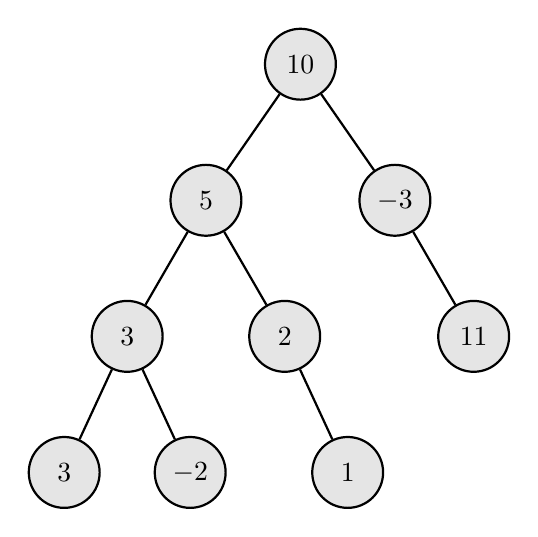
\begin{tikzpicture}
[my/.style={draw, circle, minimum size=9mm, fill=gray!20!}, thick]
\node[my](0) at(0,0) {10};
\node[my](1) [below=8mm of 0, xshift=-12mm] {5};
\node[my](2) [below=8mm of 0, xshift=12mm] {$-3$};
\node[my](3) [below=8mm of 1, xshift=-10mm] {3};
\node[my](4) [below=8mm of 1, xshift=10mm] {2};
\node[my](5) [below=8mm of 2, xshift=10mm] {11};
\node[my](6) [below=8mm of 3, xshift=-8mm] {3};
\node[my](7) [below=8mm of 3, xshift=8mm] {$-2$};
\node[my](8) [below=8mm of 4, xshift=8mm] {1};
\draw (0) -- (1);
\draw (0) -- (2);
\draw (1) -- (3);
\draw (1) -- (4);
\draw (2) -- (5);
\draw (3) -- (6);
\draw (3) -- (7);
\draw (4) -- (8);
\end{tikzpicture}
\end{figure}

$t = 8$

\textbf{Output}: 3


\textbf{Explanation}:

The paths that sum to 8 are:

\begin{enumerate}
\item $5 \longrightarrow 3$
\item $5 \longrightarrow 2 \longrightarrow 1$
\item $-3 \longrightarrow 11$
\end{enumerate}

\end{flushleft}

\setcounter{lstlisting}{0}
\begin{lstlisting}[style=customc, caption={Hash Map}]
int pathSum( TreeNode* root, int sum )
{

    unordered_map<int, int> m;
    m.emplace( 0, 1 );

    int count = 0;
    dfs( root, sum, 0, m, count );
    return count;
}
//depth first search
//the path sum
void dfs( TreeNode* node, int sum, int total, unordered_map<int, int>& m, int& count )
{
    if( !node )
    {
        return;
    }

    total += node->val;

    //find how many previous path can produce
    //sum equal to (total - sum)
    //this means how many path can produce sum
    //to current node
    auto it = m.find( total - sum );

    if( it != m.end() )
    {
        count += it->second;
    }

    it = m.find( total );
    if( it == m.end() )
    {
        it = m.emplace( total, 0 ).first;
    }

    //increments the number of path
    //that can produce total
    ++it->second;

    dfs( node->left, sum, total, m, count );
    dfs( node->right, sum, total, m, count );

    //decrements the number of path
    //that can produce total, since we will
    //leave node
    --it->second;
}
\end{lstlisting}
%\section{438 --- Find All Anagrams in a String}
Given a string $ s $ and a non-empty string $ p $, find all the start indices of $ p $'s anagrams in $ s $.

Strings consists of lowercase English letters only and the length of both strings $s$ and $p$ will not be larger than 20,100.

The order of output does not matter.

\paragraph{Example 1:}

\begin{flushleft}
\textbf{Input}: $s = \texttt{cbaebabacd}$,  $p=\texttt{abc}$

\textbf{Output}: $[0, 6]$

\textbf{Explanation}:

The substring with start index 0 is \texttt{cba}, which is an anagram of \texttt{abc}.

The substring with start index 6 is \texttt{bac}, which is an anagram of \texttt{abc}.
\end{flushleft}


\paragraph{Example 2:}

\begin{flushleft}
\textbf{Input}: $s=\texttt{abab}$, $p= \texttt{ab}$

\textbf{Output}: $[0, 1, 2]$

\textbf{Explanation}:

The substring with start index 0 is \texttt{ab}, which is an anagram of \texttt{ab}.

The substring with start index 1 is \texttt{ba}, which is an anagram of \texttt{ab}.

The substring with start index 2 is \texttt{ab}, which is an anagram of \texttt{ab}.
\end{flushleft}


\setcounter{lstlisting}{0}
\begin{lstlisting}[style=customc, caption={Sliding Window}]
vector<int> findAnagrams( string s, string p )
{
    //create the character counter
    unordered_map<int, int> m;
    for( auto c : p )
    {
        int ci = c - 'a';
        auto it = m.find( ci );
        if( it == m.end() )
        {
            m.emplace( ci, 1 );
        }
        else
        {
            ++it->second;
        }
    }

    //sliding window left and right boundary
    int l = 0;
    int r = 0;

    int lp = static_cast<int>( p.size() );
    int ls = static_cast<int>( s.size() );

    //the number of unique characters
    int count = static_cast<int>( m.size() );

    vector<int> ans;

    while( r < ls )
    {
        int ci = s[r] - 'a';
        auto it = m.find( ci );
        if( it != m.end() )
        {

            --it->second;
            if( it->second == 0 )
            {
                //This means we already
                //reach the count of character in p
                --count;
            }
        }

        ++r;

        while( count == 0 )
        {
            //now, s[l...r] contains all same
            //characters in p,
            //but may contain other letters
            int ci = s[l] - 'a';
            auto it = m.find( ci );

            if( it != m.end() )
            {
                ++it->second;
                if( it->second > 0 )
                {
                    //this letter is in p,
                    //and will be removed
                    //from current sliding window
                    //as left boundary is moving rightwards
                    ++count;
                }
            }

            //now s[l..r] is anagram of p
            if( r - l == lp )
            {
                ans.push_back( l );
            }

            ++l;
        }
    }
    return ans;
}
\end{lstlisting}
%\section{439 --- Ternary Expression Parser}
\textcolor{red}{LOCKED} 

Given a string representing arbitrarily nested ternary expressions, calculate the result of the expression. You can always assume that the given expression is valid and only consists of digits 0--9, ?, :, $T$ and $F$ ($T$ and $F$r epresent \texttt{True} and \texttt{False} respectively).

\paragraph{Note:}

\begin{itemize}
\item The length of the given string is $\leq 10000$.
\item Each number will contain only one digit.
\item The conditional expressions group right-to-left (as usual in most languages).
\item The condition will always be either \texttt{T} or \texttt{F}. That is, the condition will never be a digit.
\item The result of the expression will always evaluate to either a digit 0--9, \texttt{T} or \texttt{F}.
\end{itemize}
 

\paragraph{Example 1:}

\begin{flushleft}
\textbf{Input}: $T?2:3$

\textbf{Output}: 2

\textbf{Explanation}: If \texttt{true}, then result is 2; otherwise result is 3.
\end{flushleft}
 

\paragraph{Example 2:}

\begin{flushleft}
\textbf{Input}: $F?1:T?4:5$

\textbf{Output}: 4

\textbf{Explanation}: The conditional expressions group right-to-left. Using parenthesis, it is read/evaluated as:

$(F ? 1 : (T ? 4 : 5)) \longrightarrow (F ? 1 : 4) \longrightarrow 4$

or

$(F ? 1 : (T ? 4 : 5)) \longrightarrow (T ? 4 : 5) \longrightarrow 4$
 
\end{flushleft}


\paragraph{Example 3:}

\begin{flushleft}
\textbf{Input}: $T?T?F:5:3$

\textbf{Output}: $F$

\textbf{Explanation}: The conditional expressions group right-to-left. Using parenthesis, it is read/evaluated as:

$(T ? (T ? F : 5) : 3) \longrightarrow (T ? F : 3) \longrightarrow F$

or

$(T ? (T ? F : 5) : 3) \longrightarrow (T ? F : 5) \longrightarrow F$
\end{flushleft}

\subsection{Stack}
\begin{itemize}
\item 将expression中每个问号的index放入一个栈中,这样栈顶的问号就是表达式中最右边的问号。
\item 然后开始处理栈,每次根据顶端的index $p$,处理$s[p-1...p+1]$段的三元表达式。然后压缩expression,因为这段表达式已经处理了。
\item 将表达式的结果放入$s[p-1]$,同时将$s[p+4...L-1]$的部分往前移动4位,即$s[i-4]=s[i]$。
\item 上述移动不会影响栈中的index位置,因为这些index都位于$p-1$之前。
\end{itemize}

\setcounter{lstlisting}{0}
\begin{lstlisting}[style=customc, caption={Stack}]
string parseTernary( string expression )
{
    stack<size_t> stk;

    //push each ?'s index into stack
    for( size_t i = 0; i < expression.size(); ++i )
    {
        if( expression[i] == '?' )
        {
            stk.push( i );
        }
    }

    while( !stk.empty() )
    {
        //evaluate expression based on current position p
        //expression[p-1] is T/F
        //expression[p+1...p+3] is the ternary expression
        auto p = stk.top();
        stk.pop();

        char x = expression[p - 1];
        char y = expression[p + 1];
        if( x == 'F' )
        {
            y = expression[p + 3];
        }

        //compress the string
        //remove from s[p...p+3]
        //set s[p-1] to the result
        expression[p - 1] = y;

        //move expression[p+4...] backward by 4 positions
        for( size_t i = p + 4; i < expression.size(); ++i )
        {
            expression[i - 4] = expression[i];
        }

        //remove unnecessary parts
        expression.resize( expression.size() - 3 );
    }

    string ans;
    ans.push_back( expression[0] );
    return ans;
}
\end{lstlisting}
%\section{440 --- K-th Smallest in Lexicographical Order}
Given integers $n$ and $k$, find the lexicographically $k$-th smallest integer in the range from 1 to $n$.

\paragraph{Note:} 
\begin{itemize}
\item $1 \leq k \leq n \leq 109$.
\end{itemize}

\paragraph{Example:}

\begin{flushleft}
\textbf{Input}: $n=13$, $k=2$

\textbf{Output}:10

\textbf{Explanation}: The lexicographical order is $[1, 10, 11, 12, 13, 2, 3, 4, 5, 6, 7, 8, 9]$, so the second smallest number is 10.
\end{flushleft}

\subsection{十叉树}
数字的字典序可以用如下的十叉树来表示
\begin{figure}[H]
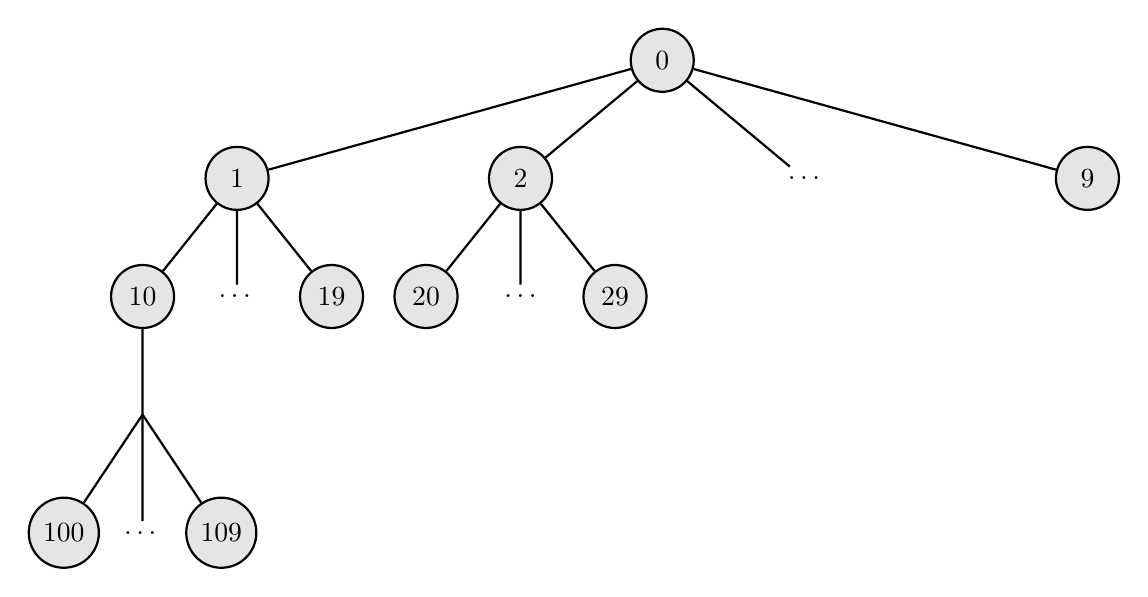
\begin{tikzpicture}
[my/.style={draw, minimum size=8mm, circle, fill=gray!20!}, thick,
level 1/.style={sibling distance=36mm}, level 2/.style={sibling distance= 12mm}, level 3/.style={sibling distance=10mm}]
\node[my](0) at (0,0) {0} 
child{
node[my] {1} 
child{
node[my] {10}
child{
	child {node[my] {100}}
	child {node {\ldots}}
	child {node[my] {109}}	
}
}
child{node {\ldots}}
child{node[my] {19}}
}
child{
node[my] {2}
child {node[my] {20}}
child {node {$\ldots$}}
child {node[my] {29}}
}
child{node(3) {$\ldots$}}
child{node[my](4) {9}};
\end{tikzpicture}
\end{figure}
preorder traverse这个tree就可以得到字典序。但是如果$k$很大,按照preorder traverse一个个的遍历显然是不可取的,需要找到快速jump的方法。
\begin{itemize}
\item 首先计算出从当前number $x$到$x+1$需要多少steps。
\item 如果total steps小于$k$,则表明$x$能跳到$x+1$。否则,则按照preorder遍历的方式前进一个step,而$x$跳到$x\times 10$。
\item 计算$x$和$y$之间的steps的方法: 
\begin{enumerate}
\item $x$和$y$之间的steps由$n$来决定,因为$n$决定了十叉树的深度。
\item 按照$x$和$y$在同层之间的间距来得到steps,例如$1$到$2$,在第一层,1到2的steps就是1。然后同时跳到第二层,这时候1变为10, 2变为20,10到20的steps就是10。
\item 做循环直到$x > n$,在每次循环中,计算$x$和$\min(n+1, y)$之间的差值加入到总的steps中。然后$x$和$y$同时跳到下一层,即$x\gets x\times 10$,$y\gets y\times 10$。
\item 
之所以选择$n+1$是因为$n<y$时,需要jump到$n$上。例如从$x=1$到$y=2$,$n=10$,当$x$和$y$都前进到下一层分别变为10和20,如果选择$\min(n,y)$,那么$\min(n,y)-x$就为零,但是我们需要从1跳到10这一个step。所以正确选择是$\min(n+1,y)$。
\end{enumerate}
\end{itemize}

\setcounter{lstlisting}{0}
\begin{lstlisting}[style=customc, caption={Prorder Traveseing With Jump To Tenary Tree}]
int findKthNumber( int n, int k )
{
    int total = 1;
    int x = 1;

    while( total < k )
    {
        int steps = cal_steps( n, x, x + 1 );

        if( total + steps <= k )
        {
            //since total are no larger than k
            //x can jump to x+1
            total += steps;
            x = x + 1;
        }
        else
        {
            //otherwise, jump down with one step
            //to next level by preorder traversing
            //x jump to x * 10
            ++total;
            x *= 10;
        }
    }
    return x;
}

//get steps between  x and y, and maximum number is n
int cal_steps( int n, int x, int y )
{
    long long steps = 0;

    //change to long long to avoid
    //overflow
    auto ln = static_cast<long long>( n );
    auto lx = static_cast<long long>( x );
    auto ly = static_cast<long long>( y );

    while( lx <= ln )
    {
        //notice: we need ln+1 not ln
        //to count for the step from x=n to n
        steps += ( min )( ln + 1, ly ) - lx;
        lx *= 10;
        ly *= 10;
    }

    return steps;
}
\end{lstlisting}
%\section{441 --- Arranging Coins}
You have a total of $n$ coins that you want to form in a staircase shape, where every $k$-th row must have exactly $k$ coins.

Given $n$, find the total number of full staircase rows that can be formed.

$n$ is a non-negative integer and fits within the range of a 32-bit signed integer.

\paragraph{Example 1:}

\begin{flushleft}
$n = 5$

The coins can form the following rows:

\begin{figure}[H]
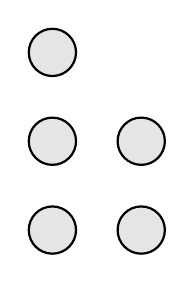
\begin{tikzpicture}
[every node/.style={draw, circle,
 minimum size=6mm, fill=gray!20!},
  node distance=5mm and 5mm, 
  every join/.style={>=stealth,->},
 thick
]
{
[start chain]
\node[on chain](0) {};
}

{
[start chain]
\node[on chain, below=of 0](1) {};
\node[on chain] {};
}

{
[start chain]
\node[on chain, below=of 1] {};
\node[on chain] {};
}
\end{tikzpicture}
\end{figure}

Because the 3rd row is incomplete, we return 2.
\end{flushleft}


\paragraph{Example 2:}

\begin{flushleft}
n = 8

The coins can form the following rows:

\begin{figure}[H]
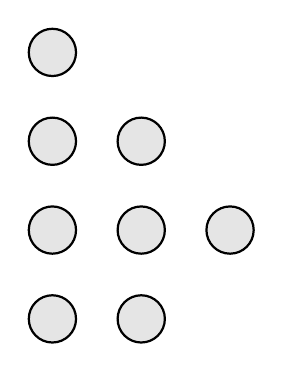
\begin{tikzpicture}
[every node/.style={draw, circle,
 minimum size=6mm, fill=gray!20!},
  node distance=5mm and 5mm, 
  every join/.style={>=stealth,->},
 thick
]
{
[start chain]
\node[on chain](0) {};
}

{
[start chain]
\node[on chain, below=of 0](1) {};
\node[on chain] {};
}

{
[start chain]
\node[on chain, below=of 1](2) {};
\node[on chain] {};
\node[on chain] {};
}

{
[start chain]
\node[on chain, below=of 2] {};
\node[on chain] {};
}
\end{tikzpicture}
\end{figure}

Because the 4th row is incomplete, we return 3.
\end{flushleft}

\subsection{Binary Search}
其实就是计算最大的整数$x$使得$x\times(x+1)/2\geq n$,可以用binary search的方式进行查找。

\setcounter{lstlisting}{0}
\begin{lstlisting}[style=customc, caption={Binary Search}]
int arrangeCoins( int n )
{
    long long l = 1;
    long long r = n;

    //left most search
    while( l < r )
    {
        long long m = ( l + r ) / 2;

        if( m * ( m + 1 ) / 2 < n )
        {
            l = m + 1;
        }
        else
        {
            r = m;
        }
    }

    //we need to check if l
    //can precisly get the to n
    auto x = ( l + 1 ) * l / 2;
    if( x == n )
    {
        return l;
    }

    return l - 1;

}
\end{lstlisting}

%\section{442 --- Find All Duplicates in an Array}
Given an array of integers, $1 \leq a[i] \leq n$ ($n$ is size of array), some elements appear twice and others appear once.

Find all the elements that appear twice in this array.

Could you do it without extra space and in $O(n)$ runtime?

\paragraph{Example:}
\begin{flushleft}
\textbf{Input}: [4,3,2,7,8,2,3,1]

\textbf{Output}: [2,3]
\end{flushleft}

\subsection{Negate Number By Its Index}
\begin{itemize}
\item Since each number is between $ [1,n] $, we can treat each element as the index in the array.
\item Iterate each element $A[i]$, set $A[A[i]] = -A[A[i]]$.
\item For the duplicate element, we will see the number at the corresponding index is negative before negating it. 
\end{itemize}

\setcounter{lstlisting}{0}
\begin{lstlisting}[style=customc, caption={Negation Index}]
vector<int> findDuplicates( vector<int>& nums )
{
    vector<int> ans;

    for( size_t i = 0; i < nums.size(); ++i )
    {
        //since nums[i] may be less than zero
        //we need absolute value of nums[i]
        //to get the index
        int idx = abs( nums[i] ) - 1;

        if( nums[idx] < 0 )
        {
            //we found duplicate elements
            //idx+1
            ans.push_back( idx + 1 );
        }
        else
        {
            //otherwise, we negate
            //the number at index idx
            nums[idx] = -nums[idx];
        }
    }

    return ans;
}
\end{lstlisting}
%\section{443 --- String Compression}
Given an array of characters $A$, compress it in-place.

The length after compression must always be smaller than or equal to the original array.

Every element of the array should be a character (not int) of length 1.

After you are done modifying the input array in-place, return the new length of the array.

 
\paragraph{Follow up:}

\begin{itemize}
\item Could you solve it using only $\mathrm{O}(1)$ extra space?
\end{itemize}

 
\paragraph{Example 1:}

\begin{flushleft}
\textbf{Input}: $[a,a,b,b,c,c,c]$

\textbf{Output}: Return 6, and the first 6 characters of the input array should be: $[a,2,b,2,c,3]$

\textbf{Explanation}: $aa$ is replaced by $a2$. $bb$ is replaced by $b2$. $ccc$ is replaced by $c3$.
 
\end{flushleft}

\paragraph{Example 2:}

\begin{flushleft}
\textbf{Input}: $[a]$

\textbf{Output}: Return 1, and the first 1 characters of the input array should be: $[a]$

\textbf{Explanation}: Nothing is replaced.

\end{flushleft}


\paragraph{Example 3:}

\begin{flushleft}
\textbf{Input}: $[a,b,b,b,b,b,b,b,b,b,b,b,b]$

\textbf{Output}: Return 4, and the first 4 characters of the input array should be: $[a,b,1,2]$.

\textbf{Explanation}: Since the character a does not repeat, it is not compressed. $bbbbbbbbbbbb$ is replaced by $b12$. Notice each digit has it's own entry in the array.
 

\end{flushleft}


\paragraph{Note:}

\begin{itemize}
\item All characters have an ASCII value in $[35, 126]$.
\item $1 \leq \lvert A\rvert \leq 1000$.
\end{itemize}

\subsection{Two Pointers}
\begin{itemize}
\item Maintain three pointers $w$, $r$ and $a$
\item $w$ is the position where we just write
\item $r$ is the position we are current at
\item $a$ is the first position of a sequence of duplicate letters
\item whenever we found different letters in two adjacent indices, this is the change of state. Write the count of duplicate letters and update $w$. And then update $a$ as the index of the new letter.
\end{itemize}

\setcounter{lstlisting}{0}
\begin{lstlisting}[style=customc, caption={Read And Write Pointers}]
int compress( vector<char>& chars )
{
    int w = 0; //write
    int a = 0; //anchor

    int L = static_cast<int>( chars.size() );

    for( int r = 0; r < L; ++r )
    {
        if( ( r + 1 == L ) || ( chars[r] != chars[r + 1] ) )
        {
            //state of change
            int count = r - a + 1;

            chars[w] = chars[a];
            ++w;

            if( count > 1 )
            {
                //write count when count
                //is larger than 1
                auto s = to_string( count );
                for( auto c : s )
                {
                    chars[w] = c;
                    ++w;
                }
            }

            //update anchor position
            a = r + 1;
        }
    }

    return w;
}
\end{lstlisting}
%\section{444 ---Sequence Reconstruction}
\textcolor{red}{\large Locked}

Check whether the original sequence $A$ can be uniquely reconstructed from the sequences in $S$. The $A$ sequence is a permutation of the integers from 1 to $n$, with $1 \leq n \leq 10^4$. Reconstruction means building a shortest common supersequence of the sequences in $S$ (i.e., a shortest sequence so that all sequences in $S$ are subsequences of it). Determine whether there is only one sequence that can be reconstructed from $S$ and it is the $A$ sequence.

\paragraph{Example 1:}

\begin{flushleft}
\textbf{Input}: $A= [1,2,3]$, $S= [\,[1,\,2],\,[1,3]\,]$

\textbf{Output}: \texttt{false}

\textbf{Explanation}:

$[1,2,3]$ is not the only one sequence that can be reconstructed, because $[1,3,2]$ is also a valid sequence that can be reconstructed.
\end{flushleft}

\paragraph{Example 2:}

\begin{flushleft}
\textbf{Input}: $A= [1,2,3]$, $S= [[1,2]]$

\textbf{Output}: \texttt{false}

\textbf{Explanation}:

The reconstructed sequence can only be $[1,2]$.
\end{flushleft}


\paragraph{Example 3:}

\begin{flushleft}
\textbf{Input}: $A = [1,2,3]$, $S = [[1,2],[1,3],[2,3]]$

\textbf{Output}: \texttt{true}

\textbf{Explanation}:

The sequences $ [1,2] $, $ [1,3] $, and $ [2,3] $ can uniquely reconstruct the original sequence $ [1,2,3] $.

\end{flushleft}

\paragraph{Example 4:}

\begin{flushleft}
\textbf{Input}: $A= [4,1,5,2,6,3]$, $S = [[5,2,6,3],[4,1,5,2]]$

\textbf{Output}: \texttt{true}
\end{flushleft}

\subsection{Verify The Position}
两个要点
\begin{itemize}
\item $A$中的elements的前后顺序在$S$中必须是一致的。
\item $A$中两个相邻元素在$S$中必定也是相邻的。
\end{itemize}

因此需要判断在$S$中的每一个sequence
\begin{enumerate}
\item 前后顺序和$A$的一致。
\item 在$S$中的所有sequence能够还原出$L-1$个adjacent element pair
\end{enumerate}

\begin{itemize}
\item 对于上述第一个判断,可以用一个数组记录$A$中每个元素的位置,然后在$S$中进行比较
\item 而对于第二个判断,则需要另外一个数组对当前元素$i$在$A$中的前面一个元素是否能够在$S$中的至少一个sequence中能够得到验证。如果能够验证,则累加验证的counter,同时标明这个元素已经被验证。最后看这个counter是否等于$L-1$。
\end{itemize}

\setcounter{lstlisting}{0}
\begin{lstlisting}[style=customc, caption={Verify The Position}]
bool sequenceReconstruction( vector<int>& org, vector<vector<int>>& seqs )
{
    vector<int> pos( org.size(), -1 );

    //verify if a element's previous element is found
    vector<unsigned char> mark( org.size(), 0 );

    int L = static_cast<int>( org.size() );

    for( int i = 0; i < L; ++i )
    {
        pos[org[i] - 1] = i;
    }

    //count is the number of adjacent elements found in seqs
    int count = 0;

    for( const auto& seq : seqs )
    {
        int l = static_cast<int>( seq.size() );

        for( int i = 0; i < l; ++i )
        {
            if( ( seq[i] > L ) || ( seq[i] <= 0 ) )
            {
                //seq[i] is out of range [0,L]
                return false;
            }

            if( i > 0 )
            {
                if( pos[seq[i - 1] - 1] >= pos[seq[i] - 1] )
                {
                    //out of order in for seq[i-1] and seq[i]
                    return false;
                }
                if( mark[seq[i] - 1] == 0 )
                {
                    //we have not mark seq[i]
                    if( pos[seq[i - 1] - 1] + 1 == pos[seq[i] - 1] )
                    {
                        //mark seq[i] is verified.
                        mark[seq[i] - 1 ] = 1;
                        //found a seq[i]'s previous number in org
                        ++count;
                    }
                }
            } //end if(i>0)
        }
    }


    //only all adjacent numbers are verified
    return count == L - 1;
}
\end{lstlisting}
%\section{445 --- Add Two Numbers II}
You are given two non-empty linked lists representing two non-negative integers. The most significant digit comes first and each of their nodes contain a single digit. Add the two numbers and return it as a linked list.

You may assume the two numbers do not contain any leading zero, except the number 0 itself.

\paragraph{Follow up:}

\begin{itemize}
\item What if you cannot modify the input lists? In other words, reversing the lists is not allowed.
\end{itemize}

\paragraph{Example:}
\begin{flushleft}

\textbf{Input}:

\begin{figure}[H]
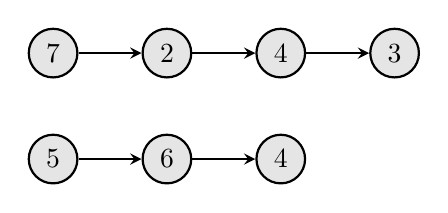
\begin{tikzpicture}
[every node/.style={draw, circle,
 minimum size=6mm, fill=gray!20!},
  node distance=8mm, 
  every join/.style={>=stealth,->},
 thick
]
{
[start chain]
\node[on chain](0) {7};
\node[on chain, join] {2};
\node[on chain, join] {4};
\node[on chain, join] {3};
}

{
[start chain]
\node[on chain,below = 7mm of 0] {5};
\node[on chain, join] {6};
\node[on chain, join] {4};
}

\end{tikzpicture}
\end{figure}

\textbf{Output}:

\begin{figure}[H]
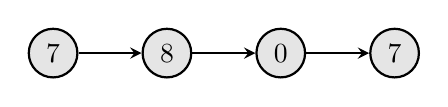
\begin{tikzpicture}
[start chain, 
every node/.style={draw, circle,
 minimum size=6mm, fill=gray!20!},
  node distance=8mm, 
  every join/.style={>=stealth,->},
 thick
]
\node[on chain] {7};
\node[on chain, join] {8};
\node[on chain, join] {0};
\node[on chain, join] {7};
\end{tikzpicture}
\end{figure}

\end{flushleft}


\subsection{Record Last Non-Nine Node}
\begin{itemize}
\item 技巧是记录链表中最后一个值不是9的node的位置,然后从这个位置往后,如果有进位发生,则该位置上的值加1,而后面的则都变为零。
\end{itemize}


\setcounter{lstlisting}{0}
\begin{lstlisting}[style=customc, caption={Record Last Non-Nine Node}]
/**
 * Definition for singly-linked list.
 * struct ListNode {
 *     int val;
 *     ListNode *next;
 *     ListNode(int x) : val(x), next(NULL) {}
 * };
 */
ListNode* addTwoNumbers( ListNode* l1, ListNode* l2 )
{

    int len1 = get_length( l1 );
    int len2 = get_length( l2 );

    //always set l1 as the longer list
    if( len1 < len2 )
    {
        swap( l1, l2 );
        swap( len1, len2 );
    }

    ListNode* dummy = new ListNode( 0 );

    auto cur = dummy;

    //the last node with value < 9
    ListNode* last = cur;

    int diff = len1 - len2;

    auto x = l1;
    auto y = l2;

    //we first link the pre-parts of l1
    while( diff )
    {
        cur->next = new ListNode( x->val );

        if( x->val != 9 )
        {
            last = cur->next;
        }

        cur = cur->next;
        x = x->next;

        --diff;
    }

    //now do addition for both lists
    while( y )
    {
        int val_x = x->val;
        int val_y = y->val;

        int sum = val_x + val_y;

        if( sum >= 10 )
        {
            sum -= 10;

            //the last node with
            //value < 9
            //increments its value
            auto z = last;
            z->val += 1;

            //set values of all nodes after this node
            //in the new list to zero
            //since 9+1=10
            while( z->next )
            {
                z->next->val = 0;
                z = z->next;
            }

            //since its value set to zero
            //this will be a possible last node
            //with value < 9
            last = z;
        }

        //Add a new node to the new list
        cur->next = new ListNode( sum );
        cur = cur->next;

        if( cur->val != 9 )
        {
            //update the last node in the new list
            //with value < 9
            last = cur;
        }

        x = x->next;
        y = y->next;
    }

    if( dummy->val == 0 )
    {
        return dummy->next;
    }

    //The first node has 1
    //we need to return the whole list
    return dummy;
}

//helper function to get length of each list
int get_length( ListNode* head )
{
    auto node = head;

    int l = 0;

    while( node )
    {
        ++l;
        node = node->next;
    }

    return l;
}

\end{lstlisting}



%\section{446 --- Arithmetic Slices II - Subsequence}
A sequence of numbers is called \textbf{arithmetic} if it consists of at least three elements and if the difference between any two consecutive elements is the same.

For example, these are arithmetic sequences:

$1, 3, 5, 7, 9$

$7, 7, 7, 7$

$3, -1, -5, -9$

The following sequence is not arithmetic.

$1, 1, 2, 5, 7$

A zero-indexed array $A$ consisting of $N$ numbers is given. A subsequence slice of that array is any sequence of integers $(P_0, P_1, \ldots, P_k)$ such that $0 \leq P_0 < P1 < \ldots < P_k < N$.

A subsequence slice $(P_0, P_1, \ldots, P_k)$ of array $A$ is called arithmetic if the sequence $A[P_0]$, $A[P_1]$, $\ldots$, $A[P_k-1]$, $A[P_k]$ is arithmetic. In particular, this means that $k \geq 2$.

The function should return the number of arithmetic subsequence slices in the array $A$.

The input contains $N$ integers. Every integer is in the range of $-2^{31}$ and $2^{31}-1$ and $0 \leq N \leq 1000$. The output is guaranteed to be less than $2^{31}-1$.
 

\paragraph{Example:}
\begin{flushleft}
\textbf{Input}: $[2, 4, 6, 8, 10]$

\textbf{Output}: 7

\textbf{Explanation}:

All arithmetic subsequence slices are:

[2,4,6]

[4,6,8]

[6,8,10]

[2,4,6,8]

[4,6,8,10]

[2,4,6,8,10]

[2,6,10]
\end{flushleft}


\subsection{Dynamic Programming}
To determine an arithmetic sequence, we need at least two parameters: the first (or last) element of the sequence, and the common difference.

Let $F[i][d]$ denotes the number of arithmetic subsequences that ends with $A[i]$ and its common difference is $d$.

Let's try to find the state transitions based on the representation above. 

\begin{itemize}
\item Assume we want to append a new element $A[i]$ to existing arithmetic subsequences to form new subsequences. We can append $A[i]$ to an existing arithmetic subsequence, only if the difference between the sequence's last element and $A[i]$ is equal to the sequence's common difference.
\item Thus, we can define the state transitions for the element A[i] as :

\[F[i][A[i] - A[j]] \gets F[i][A[i]-A[j]] +  F[j][A[i] - A[j]] \; \forall j < i\]

This demonstrates the appending process above to form new arithmetic subsequences.
\item But here comes the problem. Initially all $F[i][d]$ are 0, how to form a new arithmetic subsequence if there are no existing subsequences before?
\item In the original definition of arithmetic subsequences, the length of the subsequence must be at least 3. This makes it hard to form new subsequences if only two indices $i$ and $j$ are given. We may need to take the subsequences of length 2 into account, i.e., For any pair $i$, $j$ ($i \neq j$), $A[i]$ and $A[j]$ can always form a \textbf{weak} arithmetic subsequence.
\item Thus we can change the state representations accordingly: $F[i][d]$ denotes the number of \textbf{weak} arithmetic subsequences that ends with $A[i]$ and its common difference is $d$, the state transitions are quite straightforward:

\[F[i][A[i] - A[j]] \gets F[i][A[i]-A[j]] +  F[j][A[i] - A[j]] + 1\; \forall j < i\]

The 1 appears here because we can form a new \textbf{weak} arithmetic subsequence for the pair $(i, j)$.
\item Now the number of all weak arithmetic subsequences is the sum of all $F[i][d]$. To get the number of arithmetic subsequences that are \textbf{not weak}, we have two ways:
\begin{enumerate}
\item Count the number of \textbf{pure weak} arithmetic subsequences directly. The pure weak arithmetic subsequences are the arithmetic subsequences of length 2, so the number of pure weak arithmetic subsequences should be equal to the number of pairs $(i, j)$, which is $\dfrac{n \times (n - 1)}{2}$
\item For $F[i][A[i] - A[j]] \gets F[i][A[i]-A[j]] +  F[j][A[i] - A[j]] + 1$, $F[j][A[i] - A[j]]$ is the number of existing weak arithmetic subsequences, while 1 is the new subsequence built with $A[i]$ and $A[j]$. When appending new elements to existing weak arithmetic subsequences, we are forming arithmetic subsequences. So $F[j][A[i] - A[j]]$ is the number of new formed arithmetic subsequences, and can be added to the answer.
\end{enumerate}
\end{itemize}
Take the following example to illustrate the process:

Suppose $A =[1, 1, 2, 3, 4, 5]$

\begin{itemize}
\item For the first element 1, there is no element in front of it, the answer remains 0.

\item For the second element 1, the element itself with the previous 1 can form a pure weak arithmetic subsequence with common difference 0: $[1, 1]$.

\item For the third element 2, it cannot be appended to the only weak arithmetic subsequence $[1, 1]$, so the answer remains 0. Similar to the second element, it can form new weak arithmetic subsequences $[1, 2]$ and $[1, 2]$.

\item For the forth element 3, if we append it to some arithmetic subsequences ending with 2, these subsequences must have a common difference of $3 - 2 = 1$. Indeed there are two: $[1, 2]$ and $[1, 2]$. So we can append 3 to the end of these subsequences, and the answer is added by 2. Similar to above, it can form new weak arithmetic subsequences $[1, 3]$, $[1, 3]$ and $[2, 3]$.

\item The other elements are the same.
\end{itemize}

\setcounter{lstlisting}{0}
\begin{lstlisting}[style=customc, caption={Dynamic Programming}]
int numberOfArithmeticSlices( vector<int>& A )
{
    using ll_t = long long;

    vector<unordered_map<long long, int>> m( A.size() );

    int ans = 0;

    for( size_t i = 1; i < A.size(); ++i )
    {
        for( size_t j = 0; j < i; ++j )
        {
            auto d = static_cast<ll_t>( A[i] ) - static_cast<ll_t>( A[j] );

            //skip the difference that is overflow integer type
            if( diff > INT_MAX || diff < INT_MIN )
            {
                continue;
            }

            int count = 0;

            //find F[j][d]
            auto it = m[j].find( diff );

            if( it != m[j].end() )
            {
                count = it->second;
            }

            //the number of arithmetic subsequence
            //ending A[i] with difference = diff
            //is same as the number of arithemtic subsequence
            //ending A[j] with difference = diff
            ans += count;

            //update F[i][d]
            it = m[i].find( diff );

            //plus one because a new arithmetic subsequence
            //starting with a[j] and ending with a[i]

            if( it == m[i].end() )
            {
                m[i].emplace( diff, count + 1 );
            }
            else
            {
                it->second += ( count + 1 );
            }
        }
    }

    return ans;
}
\end{lstlisting}

%\section{447 --- Number of Boomerangs}
Given $n$ points in the plane that are all pairwise distinct, a \textbf{boomerang} is a tuple of points $(i, j, k)$ such that the distance between $i$ and $j$ equals the distance between $i$ and $k$ (the order of the tuple matters).

Find the number of \textbf{boomerang}s. You may assume that $n$ will be at most 500 and coordinates of points are all in the range $[-10000, 10000]$ (inclusive).

\paragraph{Example:}

\begin{flushleft}
\textbf{Input}: $[\, [0,0],[1,0],[2,0]\,]$

\textbf{Output}: 2

\textbf{Explanation}: The two boomerangs are $[\,[1,0],[0,0],[2,0]\,]$ and $[\,[1,0],[2,0],[0,0]\,]$

\end{flushleft}

\subsection{Hash Map}
\begin{itemize}
\item 对每一个点,计算其他所有点到这个点的距离,然后maintain一个hash map用来记录到这个点具有相同的距离的点的个数。
\item 在计算出所有的点后, 统计hash map中每个距离对应的点的个数,suppose it is $n$,那么这些点可以形成$n\times (n-1)/2$个pair,再和当前点构成bommerang。
因此结果要加上$n\times (n-1)/2$。
\end{itemize}

\setcounter{lstlisting}{0}
\begin{lstlisting}[style=customc, caption={Hash Map}]
int numberOfBoomerangs( vector<vector<int>>& points )
{
    int ans = 0;

    for( size_t i = 0; i < points.size(); ++i )
    {
        unordered_map<int, int> m;

        for( size_t j = 0; j < points.size(); ++j )
        {
            if( i == j )
            {
                continue;
            }
            auto& pi = points[i];
            auto& pj = points[j];

            int sq_dist = ( pi[0] - pj[0] ) * ( pi[0] - pj[0] ) + ( pi[1] - pj[1] ) * ( pi[1] - pj[1] );

            //add to the hash map
            //per the disance
            auto it = m.find( sq_dist );

            if( it == m.end() )
            {
                m.emplace( sq_dist, 1 );
            }
            else
            {
                it->second += 1;
            }
        }

        for( const auto& p : m )
        {
            int x = p.second;
            ans += x * ( x - 1 );
        }
    }

    return ans;
}
\end{lstlisting}
%\section{448 --- Find All Numbers Disappeared in an Array}
Given an array of integers where $1 \leq A[i] \leq$ ($n  = \lvert A\rvert$), some elements appear twice and others appear once.

Find all the elements of $[1, n]$ inclusive that do not appear in this array.

Could you do it without extra space and in $O(n)$ runtime? You may assume the returned list does not count as extra space.

\paragraph{Example:}

\begin{flushleft}
\textbf{Input}:

$[4,3,2,7,8,2,3,1]$

\textbf{Output}:

$[5,6]$

\end{flushleft}

\paragraph{Note}
\begin{itemize}
\item Refer to problem \textbf{442}
\end{itemize}

\setcounter{lstlisting}{0}
\begin{lstlisting}[style=customc, caption={Using Index As Key}]
vector<int> findDisappearedNumbers( vector<int>& nums )
{
    int N = static_cast<int>( nums.size() );

    for( int i = 0; i < N; ++i )
    {
        int x = abs( nums[i] );

        if( nums[x - 1] > 0 )
        {
            //only change to negative
            //when it is negative
            nums[x - 1] = -nums[x - 1];
        }
    }

    vector<int> ans;

    for( int i = 0; i < N; ++i )
    {
        if( nums[i] > 0 )
        {
            //the index that has positive element
            //is the one of the result
            ans.push_back( i + 1 );
        }
    }

    return ans;
}
\end{lstlisting}
%\section{449 --- Serialize and Deserialize BST}
Serialization is the process of converting a data structure or object into a sequence of bits so that it can be stored in a file or memory buffer, or transmitted across a network connection link to be reconstructed later in the same or another computer environment.

Design an algorithm to serialize and deserialize a \textbf{binary search tree}. There is no restriction on how your serialization/deserialization algorithm should work. You just need to ensure that a binary search tree can be serialized to a string and this string can be deserialized to the original tree structure.

\textbf{The encoded string should be as compact as possible.}

\paragraph{Note:} 
\begin{itemize}
\item Do not use class member/global/static variables to store states. Your serialize and deserialize algorithms should be stateless.
\end{itemize}

\subsection{Postorder traversal to optimise space for the tree structure}
BST could be constructed from preorder or postorder traversal only. In brief, it's a consequence of two facts:

\begin{itemize}
\item Binary tree could be constructed from preorder/postorder and inorder traversal.
\item Inorder traversal of BST is an array sorted in the ascending order: inorder is sorted preorder sequence.
\end{itemize}
That means that BST structure is already encoded in the preorder or postorder traversal and hence they are both suitable for the compact serialization.

Serialization could be easily implemented with both strategies, in this case, preorder can be implemented more efficiently.

\setcounter{lstlisting}{0}
\begin{lstlisting}[style=customc, caption={preorder}]
class Codec
{
public:

    // Encodes a tree to a single string.
    string serialize( TreeNode* root )
    {

        string s;

        //serialize by preorder travese
        preorder( root, s );

        if( !s.empty() )
        {
            //remove last blanck
            s.pop_back();
        }


        return s;
    }

    void preorder( TreeNode* node, string& s )
    {
        if( !node )
        {
            return;
        }

        s += to_string( node->val );
        s.push_back( ' ' );


        preorder( node->left, s );
        preorder( node->right, s );

    }




    // Decodes your encoded data to tree.
    TreeNode* deserialize( string data )
    {
        size_t start = 0;
        return build( data, start, INT_MIN, INT_MAX );
    }

    //from characters to integer
    int get_val( const char*s, size_t start, size_t end )
    {
        int x = 0;
        for( size_t i = start; i < end; ++i )
        {
            x = x * 10 + ( s[i] - '0' );
        }

        return x;
    }

    //we need start as a reference type
    //because we need this parameter to be changed
    //during the recursion, so that the index in s can
    //move forward
    TreeNode* build( string& s, size_t& start, int low, int up )
    {
        if( start >= s.size() )
        {
            return nullptr;
        }

        //find index of next space
        auto pos = s.find( ' ', start );

        if( pos == string::npos )
        {
            pos = s.size();
        }

        int val = get_val( s.c_str(), start, pos );


        if( ( val < low ) || ( val > up ) )
        {
            return nullptr;
        }

        //update next search start index
        start = pos + 1;

        TreeNode* node = new TreeNode( val );
        //after left is done
        //start will be updated
        node->left = build( s, start, low, val );

        node->right = build( s, start, val, up );

        return node;
    }
};
\end{lstlisting}


%\section{450 --- Delete Node in a BST}
Given a root node reference of a BST and a key $x$, delete the node with the given key in the BST. Return the root node reference (possibly updated) of the BST.

Basically, the deletion can be divided into two stages:

\begin{itemize}
\item Search for a node to remove.
\item If the node is found, delete the node.
\end{itemize}

\paragraph{Note:} 
\begin{itemize}
\item Time complexity should be O(height of tree).
\end{itemize}

\paragraph{Example:}
\begin{flushleft}
\textbf{Input}: 
\begin{figure}[H]
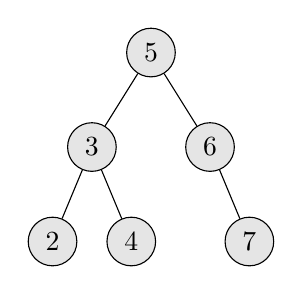
\begin{tikzpicture}
[every node/.style={draw, circle, fill=gray!20!, minimum size=5mm},
level 2/.style ={sibling distance=1cm}, 
level 3/.style={sibling distance=8mm},
level distance=1.2cm]
\node {5}
 child{ node(a){3} child { node {2} } child { node {4} }   } 
%
 child{ node(b){6} child[missing] {} child { node {7} } };
%;
\end{tikzpicture}
\end{figure}
$x = 3$

\textbf{Output}: 
One valid answer is shown in the following BST.

\begin{figure}[H]
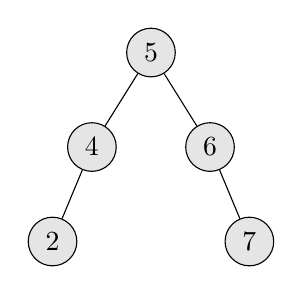
\begin{tikzpicture}
[every node/.style={draw, circle, fill=gray!20!, minimum size=5mm},
level 2/.style ={sibling distance=1cm}, 
level 3/.style={sibling distance=8mm},
level distance=1.2cm]
\node {5}
child { node {4} child {node{2}} child[missing]{} }
child { node {6} child[missing] {} child {node{7}} };
\end{tikzpicture}
\end{figure}

Another valid answer is
\begin{figure}[H]
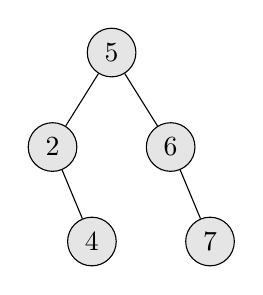
\begin{tikzpicture}
[every node/.style={draw, circle, fill=gray!20!, minimum size=5mm},
level 2/.style ={sibling distance=1cm}, 
level 3/.style={sibling distance=8mm},
level distance=1.2cm]
\node {5}
child { node {2} child[missing]{} child {node{4}} }
child { node {6} child[missing] {} child {node{7}} };
\end{tikzpicture}
\end{figure}
\end{flushleft}
%\section{451 --- Sort Characters By Frequency}
Given a string $s$, sort it in decreasing order based on the frequency of characters.

\paragraph{Example 1:}

\begin{flushleft}
\textbf{Input}: \texttt{tree}

\textbf{Output}: \texttt{eert}

\textbf{Explanation}:

\texttt{e} appears twice while \texttt{r} and \texttt{t} both appear once.

So \texttt{e} must appear before both \texttt{r} and \texttt{t}. Therefore \texttt{eetr} is also a valid answer.

\end{flushleft}

\paragraph{Example 2:}

\begin{flushleft}
\textbf{Input}: \texttt{cccaaa}

\textbf{Output}: \texttt{cccaaa}

\textbf{Explanation}:

Both \texttt{c} and \texttt{a} appear three times, so \texttt{aaaccc} is also a valid answer.

Note that \texttt{cacaca} is incorrect, as the same characters must be together.

\end{flushleft}


\paragraph{Example 3:}

\begin{flushleft}
\textbf{Input}: \texttt{Aabb}

\textbf{Output}: \texttt{bbAa}

\textbf{Explanation}:

\texttt{bbaA} is also a valid answer, but \texttt{Aabb} is incorrect.

Note that \texttt{A} and \texttt{a} are treated as two different characters.
\end{flushleft}

\subsection{Bucket Sort}
\begin{itemize}
\item The maximum frequency of a character in $s$ is the length of $s$, say $\ell$. Therefore we can create $\ell$ buckets to put same frequency characters into one bucket.
\end{itemize}

\setcounter{lstlisting}{0}
\begin{lstlisting}[style=customc, caption={Bucket Sort}]
string frequencySort( string s )
{
    unordered_map<int, int> m;
    //put characters with x frequence
    //into buckets[x-1]
    vector<string> buckets( s.size() );

    for( auto c : s )
    {
        m[c] += 1;
    }

    for( const auto& p : m )
    {
        int count = p.second;
        char c = p.first;
        //add count of c into buckets[count-1]
        buckets[count - 1].append( count, c );
    }

    string ans;
    //buckets[i] has frequence i+1
    //therefore we need to group the letters
    //from end of bucket
    for( size_t i = s.size(); i >= 1 ; --i )
    {
        if( !buckets[i - 1].empty() )
        {
            //only add non-empty
            //bucket
            ans += buckets[i - 1];
        }
    }
    return ans;
}
\end{lstlisting}
%\section{452 --- Minimum Number of Arrows to Burst Balloons}
There are a number of spherical balloons spread in two-dimensional space. For each balloon, provided input is the start and end coordinates of the horizontal diameter. Since it's horizontal, $y$-coordinates don't matter and hence the $x$-coordinates of start and end of the diameter suffice. Start is always smaller than end. There will be at most 104 balloons.

An arrow can be shot up exactly vertically from different points along the $x$-axis. A balloon with start position $\alpha$ and end position $\beta$ bursts by an arrow shot at $x$ if $\alpha \leq x\leq \beta$. There is no limit to the number of arrows that can be shot. An arrow once shot keeps traveling up infinitely. The problem is to find the minimum number of arrows that must be shot to burst all balloons.

\paragraph{Example:}

\begin{flushleft}
\textbf{Input}: $[[10,16], [2,8], [1,6], [7,12]]$

\textbf{Output}: 2

\textbf{Explanation}:

One way is to shoot one arrow for example at $x = 6$ (bursting the balloons $[2,8]$ and $[1,6]$) and another arrow at $x = 11$ (bursting the other two balloons).

\end{flushleft}

\subsection{Greedy}
\begin{itemize}
\item This is a deviation of a problem that find the overlapped ranges
\item At start, sort the input ranges per the end position.
\item Set first end $y$ as the first range's end position in the sorted ranges. Iterate all the other ranges, if a range's start position is no larger than $y$, we know that an arrow can burst them together. Otherwise, increments the number of arrows.
\item The difference between this problem and the problem that find overlapped ranges, we do not update $y$ as the merged range's end position. We leave $y$ as it is. 
\end{itemize}

\setcounter{lstlisting}{0}
\begin{lstlisting}[style=customc, caption={Greedy}]
int findMinArrowShots( vector<vector<int>>& points )
{
    if( points.empty() )
    {
        return 0;
    }

    //sort the points per the end position
    sort( begin( points ), end( points ), []( const vector<int>& p1, const vector<int>& p2 )
    {
        if( p1[1] < p2[1] )
        {
            return true;
        }

        if( p1[1] == p2[1] )
        {
            return p1[0] < p2[0];
        }

        return false;
    } );

    int ans = 1;

    int end = points[0][1];

    for( size_t i = 1; i < points.size(); ++i )
    {
        if( points[i][0] <= end )
        {
            //point i can be burst together
            //notice: we do not update end
            //as in finding overlapped ranges
        }
        else
        {
            //we need another arrow
            ++ans;
            end = points[i][1];
        }
    }

    return ans;
}
\end{lstlisting}
%\section{453 --- Minimum Moves to Equal Array Elements}
Given a non-empty integer array $A$ of size $n$, find the minimum number of moves required to make all array elements equal, where a move is incrementing $n - 1$ elements by 1.

\paragraph{Example:}

\begin{flushleft}
\textbf{Input}: $[1,2,3]$

\textbf{Output}: 3

\textbf{Explanation}: 

Only three moves are needed (remember each move increments two elements):

$[1,2,3]  \Longrightarrow  [2,3,3]  \Longrightarrow  [3,4,3] \Longrightarrow  [4,4,4]$
\end{flushleft}

\subsection{Math}
Adding 1 to all the elements except one is equivalent to decrementing 1 from a single element, since we are interested in the relative levels of the elements which need to be equalized. Thus, the problem is simplified to find the number of decrement operations required to equalize all the elements of the given array. 

For finding this, it is obvious that we'll reduce all the elements of the array to the minimum element. But, in order to find the solution, we need not actually decrement the elements. We can find the number of moves required as $\sum\limits_{i=0}^{\ell-1} A[i] - \min(A)\times \ell$, where $\ell$ is the length of the array.

\setcounter{lstlisting}{0}
\begin{lstlisting}[style=customc, caption={Math}]
int minMoves( vector<int>& nums )
{
    //get minimum element
    auto it = min_element( begin( nums ), end( nums ) );
    auto min_e = *it;

    int ans = 0;

    //sum - min(nums) * L
    //=sum(A[i] - min(nums));
    for( int n : nums )
    {
        ans += ( n - min_e );
    }

    return ans;
}
\end{lstlisting}

\subsection{Brute Force}
In order to make all the elements equal to each other with minimum moves, we need to do the increments in all but the maximum element of the array. 

Thus, in this approach, we scan the complete array to find the maximum and the minimum element. After this, we add 1 to all the elements except the maximum element, and increment the number of moves. Again, we repeat the same process, and this continues until the maximum and the minimum element become equal to each other.

But we can do better. In order to make the minimum element equal to the maximum element, we need to add 1 at least $k$ times, after which, the maximum element could change. Thus, instead of incrementing in steps of 1, we can increase the number of moves by $ k=\max-\min$. Thus, we scan the complete array to find the maximum and minimum element. Then, we increment every element by $k$ units and add $k$ to the count of moves. Again we repeat the same process, until the maximum and minimum element become equal.

\begin{lstlisting}[style=customc, caption={Better Brute Force}]
int minMoves( vector<int>& nums )
{
    //Time Limit Exceed
    //Only for demonstration
    int ans = 0;
    while( true )
    {
        auto minmax_p = minmax_element( begin( nums ), end( nums ) );
        int min_n = *( minmax_p.first );
        int max_n = *( minmax_p.second );

        int diff = max_n - min_n;

        if( diff == 0 )
        {
            break;
        }

        ans += diff;

        for( auto it = begin( nums ); it != end( nums ); ++it )
        {
            //skip the first maximum found
            if( it != minmax_p.second )
            {
                *it += diff;
            }
        }
    }

    return ans;
}
\end{lstlisting}

\subsection{Sorting}
If the array is sorted, we can find the maximum and minimum element in $O(1)$. Actually, we don't need to update each element in $A$.

\begin{enumerate}
\item At start, the last element is the largest element. Therefore, $d = A[n-1]-A[0]$. 
\item We add $d$ to all the elements except the last one, i.e., $A[n-1]$. Now, the updated element at index 0, $A[0]$ will be $A[0]+d = A[n-1]$. Thus, the smallest element $A[0]$ is now equal to the previous largest element $A[n-1]$. Because $A$ is sorted, the element $A[n-2]$ will become the largest element after updated. Also, $A[0]$ is still the smallest element.
\item For the 2nd update, difference $d$ is $A[n-2]-A[0]$. Thus, $A[0]$ will become equal to $A[n-2]$ after update. Further, since $A[0]$ is equal to $A[n-1]$, we have $A[0]=A[n-2]=A[n-1]$. Now, the largest element will be $A[n-3]$. 

\item Continue the above steps, and keep on incrementing the number of moves with the difference found at every step.
\end{enumerate}
%\section{454 --- 4Sum II}
Given four lists $A$, $B$, $C$, $D$ of integer values, compute how many tuples $(i, j, k, l)$ there are such that $A[i] + B[j] + C[k] + D[l]$ is zero.

To make problem a bit easier, all $A, B, C, D$ have same length of $N$ where $0 \leq N \leq 500$. All integers are in the range of $-2^{28}$ to $2^{28} - 1$ and the result is guaranteed to be at most $2^{31} - 1$.

\paragraph{Example:}

\begin{flushleft}
\textbf{Input}:

$A = [ 1, 2],\, B = [-2,-1],\, C = [-1, 2], \,D = [ 0, 2]$

\textbf{Output}: 2

\textbf{Explanation}:

The two tuples are:

\begin{enumerate}
\item $(0, 0, 0, 1) \longrightarrow A[0] + B[0] + C[0] + D[1] = 1 + (-2) + (-1) + 2 = 0$
\item $(1, 1, 0, 0) -> A[1] + B[1] + C[0] + D[0] = 2 + (-1) + (-1) + 0 = 0$
\end{enumerate}
\end{flushleft}

\subsection{Hash Map}

\begin{itemize}
\item Put the sum of all the element pairs from $A$ and $B$ into a hash map $M$.
\item Then the problem reduced to find the sum of two numbers from $C$ and $D$, say $x$, so that $-x$ can be found in $M$.
\end{itemize}

\setcounter{lstlisting}{0}
\begin{lstlisting}[style=customc, caption={hash map}]
int fourSumCount( vector<int>& A, vector<int>& B, vector<int>& C, vector<int>& D )
{
    unordered_map<int, int> m;

    //get the sum of A[i]+[j]
    for( size_t i = 0; i < A.size(); ++i )
    {
        for( size_t j = 0; j < B.size(); ++j )
        {
            int sum = A[i] + B[j];

            auto it = m.find( sum );

            if( it == m.end() )
            {
                m.emplace( sum, 1 );
            }
            else
            {
                it->second += 1;
            }
        }
    }
    int ans = 0;
    //find if C[k]+D[l]=-A[i]-B[j]
    for( size_t i = 0; i < C.size(); ++i )
    {
        for( size_t j = 0; j < D.size(); ++j )
        {
            int sum = C[i] + D[j];
            auto it = m.find( -sum );

            if( it != m.end() )
            {
                //each pair (i,j) will have a unique combination
                //with current (k,l)
                ans += it->second;
            }
        }
    }
    return ans;
}
\end{lstlisting}

%\section{455 --- Assign Cookies}
Assume you are an awesome parent and want to give your children some cookies. But, you should give each child at most one cookie. Each child $i$ has a greed factor $g_i$, which is the minimum size of a cookie that the child will be content with; and each cookie $j$ has a size $s_j$. If $s_j \geq g_i$, we can assign the cookie $j$ to the child $i$, and the child $i$ will be content. Your goal is to maximize the number of your content children and output the maximum number.

\paragraph{Note:}
\begin{itemize}
\item You may assume the greed factor is always positive.
\item You cannot assign more than one cookie to one child.
\end{itemize}


\paragraph{Example 1:}

\begin{flushleft}
\textbf{Input}: $g=[1,2,3]$, $s=[1,1]$

\textbf{Output}: 1

\textbf{Explanation}: 

You have 3 children and 2 cookies. The greed factors of 3 children are 1, 2, 3. And even though you have 2 cookies, since their size is both 1, you could only make the child whose greed factor is 1 content.

You need to output 1.
\end{flushleft}

\paragraph{Example 2:}

\begin{flushleft}
\textbf{Input}: $g=[1,2]$, $s=[1,2,3]$

\textbf{Output}: 2

\textbf{Explanation}: 

You have 2 children and 3 cookies. The greed factors of 2 children are 1, 2. You have 3 cookies and their sizes are big enough to gratify all of the children, You need to output 2.
\end{flushleft}

\subsection{Sorting And Binary Search}

\setcounter{lstlisting}{0}
\begin{lstlisting}[style=customc, caption={Binary Search}]
int findContentChildren( vector<int>& g, vector<int>& s )
{

    //we need binary search
    //sort both first
    sort( g.begin(), g.end() );

    sort( s.begin(), s.end() );

    int ans = 0;

    //the search start in g
    int last = 0;

    //we need to find which cookie can satisfy
    for( int x : g )
    {
        int l = last;
        int r = static_cast<int>( s.size() );

        if( l == r )
        {
            break;
        }

        //leftmost binary search
        while( l < r )
        {
            int mid = ( l + r ) / 2;

            if( s[mid] < x )
            {
                l = mid + 1;
            }
            else
            {
                r = mid;
            }
        }

        if( l < static_cast<int>( s.size() ) )
        {
            //this cookie can be
            //consumed by current child with greed x
            ++ans;
        }
        else
        {
            //otherwise, since greedy is sorted,
            //no cookie can satisfy any more child
            break;
        }


        //since the cookie is consumed
        //set the start of search to the next one
        last = l + 1;

    }

    return ans;
}
\end{lstlisting}

%\section{456 --- 132 Pattern}
Given a sequence of $n$ integers $a_1$, $a_2$, $\ldots$, $a_n$, a 132 pattern is a subsequence $a_i$, $a_j$, $a_k$ such that $i < j < k$ and $a_i < a_k < a_j$. Design an algorithm that takes a list of $n $ numbers as input and checks whether there is a 132 pattern in the list.

Note: $n$ will be less than 15,000.

\paragraph{Example 1:}

\begin{flushleft}
\textbf{Input}: [1, 2, 3, 4]

\textbf{Output}: \texttt{False}

\textbf{Explanation}: There is no 132 pattern in the sequence.
\end{flushleft}

\paragraph{Example 2:}

\begin{flushleft}
\textbf{Input}: [3, 1, 4, 2]

\textbf{Output}: \texttt{True}

\textbf{Explanation}: There is a 132 pattern in the sequence: $[1, 4, 2]$.
\end{flushleft}

\paragraph{Example 3:}

\begin{flushleft}
\textbf{Input}: [-1, 3, 2, 0]

\textbf{Output}: \texttt{True}

\textbf{Explanation}: There are three 132 patterns in the sequence: [-1, 3, 2], [-1, 3, 0] and [-1, 2, 0].

\end{flushleft}

\setcounter{lstlisting}{0}
\begin{lstlisting}[style=customc, caption={Stack}]
bool find132pattern( vector<int>& nums )
{
    if( nums.empty() || ( nums.size() < 3 ) )
    {
        return false;
    }

    int L = static_cast<int>( nums.size() );

    int x_k = INT_MIN;

    stack<int> stk;

    for( int i = L - 1; i >= 0; --i )
    {
        //stk is not empty means
        //we have x_j > x_k and (j < k)
        //so if x_i < x_k is found
        //we found the pattern
        if( !stk.empty() && ( nums[i] < x_k ) )
        {
            return true;
        }

        //we put x_j in the stack
        //pop all numbers in the stack that is less than nums[i]
        //the last one will be the latest x_k < x_j
        //this is strict less than, so we use
        //stk.top() < nums[i]
        while( !stk.empty() && ( stk.top() < nums[i] ) )
        {
            //update x_k as the top of the stack
            x_k = stk.top();
            stk.pop();
        }

        //now the numbers in the stack
        //are larger than x_k
        stk.push( nums[i] );
    }

    return false;
}
\end{lstlisting}
%\section{457 --- Circular Array Loop}
You are given a circular array $A$ of positive and negative integers. If a number $ k $ at an index is positive, then move forward $k$ steps. Conversely, if it's negative ($-k$), move backward $k$ steps. Since the array is circular, you may assume that the last element's next element is the first element, and the first element's previous element is the last element.

Determine if there is a loop (or a cycle) in $A$. A cycle must start and end at the same index and the cycle's length is larger than 1. Furthermore, movements in a cycle must all follow a single direction. In other words, a cycle must not consist of both forward and backward movements.

 
\paragraph{Example 1:}

\begin{flushleft}
\textbf{Input}: [2,-1,1,2,2]

\textbf{Output}: \texttt{true}

\textbf{Explanation}: There is a cycle, from index $0 \longrightarrow 2 \longrightarrow 3 \longrightarrow 0$. The cycle's length is 3.
\end{flushleft}


\paragraph{Example 2:}

\begin{flushleft}
\textbf{Input}: [-1,2]

\textbf{Output}: \texttt{false}

\textbf{Explanation}: The movement from index $1 \longrightarrow 1 \longrightarrow 1 \ldots$ is not a cycle, because the cycle's length is 1. By definition the cycle's length must be greater than 1.

\end{flushleft}


\paragraph{Example 3:}

\begin{flushleft}
\textbf{Input}: [-2,1,-1,-2,-2]

\textbf{Output}: \texttt{false}

\textbf{Explanation}: The movement from index $1 \longrightarrow 2 \longrightarrow 1 \longrightarrow \ldots$ is not a cycle, because movement from index $1 \longrightarrow 2$ is a forward movement, but movement from index $2 \longrightarrow 1$ is a backward movement. All movements in a cycle must follow a single direction.
\end{flushleft}
 

\paragraph{Note:}

\begin{itemize}
\item $-1000 \leq A[i] \leq 1000$
\item $A[i] \neq 0$
\item $1 \leq \lvert A\rvert \leq 5000$
 \end{itemize}

\paragraph{Follow up:}

\begin{itemize}
\item Could you solve it in $O(n)$ time complexity and $O(1)$ extra space complexity?
\end{itemize}

\setcounter{lstlisting}{0}
\begin{lstlisting}[style=customc, caption={Fast And Slow Pointers}]
bool circularArrayLoop( vector<int>& nums )
{

    int L = static_cast<int>( nums.size() );

    auto next = [L, &nums]( int x )
    {

        int y = x + nums[x];
        y = ( y % L );

        if( y < 0 )
        {
            y += L;
        }

        return y;
    };

    //start from each index
    //to see if there is a loop
    for( int i = 0; i < L; ++i )
    {
        if( nums[i] == 0 )
        {
            continue;
        }

        int slow = i;
        int fast = next( i );

        //fast will jump two index
        //so make sure these two index has
        //same directions as i
        while( ( nums[fast] * nums[i] > 0 ) && ( nums[next( fast )] * nums[i] > 0 ) )
        {
            if( slow == fast )
            {
                //the loop contains only element
                if( slow == next( slow ) )
                {
                    break;
                }

                //we found a loop
                return true;
            }

            //jump one index for slow
            slow = next( slow );
            //jump two index for fast
            fast = next( next( fast ) );
        }


        //we cannot find loop starting from i
        int x = i;
        int val = nums[i];
        //set the elements in the path from i to zero
        while( nums[x] * val > 0 )
        {
            //nums[x] needs to be the
            //same direction as x
            int y = next( x );
            nums[x] = 0;
            x = y;
        }
    }

    return false;
}

\end{lstlisting}
%\section{458 --- Poor Pigs}
There are 1000 buckets, one and only one of them is poisonous, while the rest are filled with water. They all look identical. If a pig drinks the poison it will die within 15 minutes. What is the minimum amount of pigs you need to figure out which bucket is poisonous within one hour?

Answer this question, and write an algorithm for the general case.

\paragraph{General case:}

\begin{flushleft}
If there are $n$ buckets and a pig drinking poison will die within $m$ minutes, how many pigs ($x$) you need to figure out the poisonous bucket within $p$ minutes? There is exactly one bucket with poison.
\end{flushleft}

 
\paragraph{Note:}

\begin{itemize}
\item A pig can be allowed to drink simultaneously on as many buckets as one would like, and the feeding takes no time.
\item After a pig has instantly finished drinking buckets, there has to be a cool down time of $
m$ minutes. During this time, only observation is allowed and no feedings at all.
\item Any given bucket can be sampled an infinite number of times (by an unlimited number of pigs).
\end{itemize}

\subsection{Matrix}
With 2 pigs, poison killing in 15 minutes, and having 60 minutes, we can find the poison in up to 25 buckets in the following way. Arrange the buckets in a $5\times 5$ square:

\[ 
\begin{bmatrix}
1 & 2 & 3 & 4 & 5 \\
6 & 7 & 8 & 9 & 10 \\
11 & 12 & 13 & 14 & 15 \\
16 & 17 & 18 & 19 & 20 \\
21 & 22 & 23 & 24 & 25
\end{bmatrix}
 \]
 
Now use one pig to find the row (make it drink from buckets 1, 2, 3, 4, 5, wait 15 minutes, make it drink from buckets 6, 7, 8, 9, 10, wait 15 minutes, etc). Use the second pig to find the column (make it drink 1, 6, 11, 16, 21, then 2, 7, 12, 17, 22, etc).

Having 60 minutes and tests taking 15 minutes means we can run four tests. If the row pig dies in the third test, the poison is in the third row. If the column pig doesn't die at all, the poison is in the fifth column (this is why we can cover five rows/columns even though we can only run four tests).

With 3 pigs, we can similarly use a $5\times 5\times 5$ cube instead of a $5\times 5$ square and again use one pig to determine the coordinate of one dimension (one pig drinks layers from top to bottom, one drinks layers from left to right, one drinks layers from front to back). So 3 pigs can solve up to 125 buckets.

In general, we can solve up to $(\lfloor p / m\rfloor + 1)^x$ buckets this way ($x$ is the number of pigs), so just find the smallest sufficient number of pigs $x$ such that
\[
(\lfloor p / m\rfloor + 1)^x \geq n
\]

\setcounter{lstlisting}{0}
\begin{lstlisting}[style=customc, caption={Matrix}]
int poorPigs( int buckets, int minutesToDie, int minutesToTest )
{
    int x = 0;

    //base is the dimension of the matrix that
    //can be used to test
    int base = ( minutesToTest / minutesToDie ) + 1;
    int y = 1;
    while( y < buckets )
    {
        //increments the number of pigs
        ++x;
        y *= base;
    }

    return x;
}
\end{lstlisting}
%\section{459 --- Repeated Substring Pattern}
Given a non-empty string, $S$, check if it can be constructed by taking a substring of it and appending multiple copies of the substring together. You may assume the given string consists of lowercase English letters only and its length will not exceed 10000.

\paragraph{Example 1:}

\begin{flushleft}
\textbf{Input}: $ abab $

\textbf{Output}: \texttt{True}

\textbf{Explanation}: It's the substring $ ab $ twice.

\end{flushleft}

\paragraph{Example 2:}

\begin{flushleft}
\textbf{Input}: $ aba $

\textbf{Output}: \texttt{False}
\end{flushleft}


\paragraph{Example 3:}

\begin{flushleft}
\textbf{Input}: $ abcabcabcabc $

\textbf{Output}: \texttt{True}

\textbf{Explanation}: It's the substring $ abc $ four times. (And the substring $ abcabc $ twice.)

\end{flushleft}

\subsection{KMP}
\begin{itemize}
\item We build KMP table $T$ first from $S$.
\item Any entry in KMP table, $T[i]$, is the length of longest proper prefix of $S[0,i]$, which is also a suffix of $S[0,i]$.
\item Thus $T[L-1]$ ($L$ is the length of $S$) is the length of longest proper prefix of $S$. Thus, if $S$ can be built by one of its substring, say $U$, then $U$ must be the suffix of $S$ and also the proper prefix of $S$.
\item We only need to check if $T[L-1]$ is greater than zero and $L$ is the multiple of $L-T[L-1]$.  
\end{itemize}

\setcounter{lstlisting}{0}
\begin{lstlisting}[style=customc, caption={KMP}]
bool repeatedSubstringPattern( string s )
{
    //build kmp table
    vector<size_t> f( s.size(), 0 );

    for( size_t i = 1; i < s.size(); ++i )
    {
        auto t = f[i - 1];

        while( ( t > 0 ) && ( s[i] != s[t] ) )
        {
            t = f[t - 1];
        }

        if( s[i] == s[t] )
        {
            t = t + 1;
        }

        f[i] = t;
    }

    //if s is made of a multiple substring t
    //then x = (r-1) * len(t) where r is the
    //count of t in x
    //so l-x is the length of the t
    //we need to make sure x is not zero
    //and l can be devided by (l-x)

    auto x = f.back();

    auto l = s.size();

    if( ( x > 0 ) && ( l % ( l - x ) == 0 ) )
    {
        return true;
    }

    return false;
}
\end{lstlisting}

\subsection{The Trick To Find A Repeatable String}
Based on this fact:
\begin{itemize}
\item First char of input string is first char of repeated sub-string
\item Last char of input string is last char of repeated sub-string
\item Assume $T = S+S$ where $S$ is the input string.
\item Remove first and last letter from $T$.
\item If $S$ exists in $T$, we know that $S$ contains a repeatable sub-string. Suppose index $i$ in $T$ is the index where $S$ starts, then the repeatable string in $S$ has length $i+1$ and the repeat sub-string in $S$ is $S[0, i]$.
\end{itemize}
%\section{460 --- LFU Cache}
Design and implement a data structure for Least Frequently Used (\texttt{LFU}) cache. It should support the following operations: \texttt{get} and \texttt{put}.

\begin{lstlisting}[style=customc]
/*
Get the value (will always be positive) of the key
if the key exists in the cache,
otherwise return -1.
*/
int get( int key );

/*
Set or insert the value if the key is not already present.
When the cache reaches its capacity, it should invalidate
the least frequently used item before inserting a new item.
For the purpose of this problem, when there is a tie
(i.e., two or more keys that have the same frequency),
the least recently used key would be evicted.
*/
void put( int key, int value );

\end{lstlisting}

\paragraph{Follow up:}

\begin{itemize}
\item Could you do both operations in O(1) time complexity?
\end{itemize}

\paragraph{Example:}

\begin{lstlisting}[style=customc]
LFUCache cache = new LFUCache( 2 /* capacity */ );

cache->put(1, 1);
cache->put(2, 2);
cache->get(1);       // returns 1
cache->put(3, 3);    // evicts key 2
cache->get(2);       // returns -1 (not found)
cache->get(3);       // returns 3
cache->put(4, 4);    // evicts key 1
cache->get(1);       // returns -1 (not found)
cache->get(3);       // returns 3
cache->get(4);       // returns 4
\end{lstlisting}

\subsection{Double Linked List And Hash Map}
注意:这里是LFU不是LRU。即如果有多个元素都是最少访问的,那么需要从中删除最近没有访问过的。

We have to make use of two lists. One list is used to store the key/value and another is used to store the frequency related key/value list. We also need a hash map to store each key and its position in the two lists.

\setcounter{lstlisting}{0}
\begin{lstlisting}[style=customc, caption={List And Hash Map}]
class LFUCache
{
public:
    LFUCache( int capacity )
    {
        m_cap = capacity;
        m_size = 0;
    }

    int get( int key )
    {
        auto p_dict = m_dict.find( key );
        if( p_dict == m_dict.end() )
        {
            return -1;
        }

        //find in m_list
        auto outer = p_dict->second.outer;
        auto inner = p_dict->second.inner;

        //save value
        int value = inner->v;

        //increments the frequency
        auto n_outer = outer;
        ++n_outer; //the next of outer;

        //erase (key, value) from outer's kv list L
        outer->L.erase( inner );

        if( ( n_outer == m_list.end() ) || ( n_outer->f != outer->f + 1 ) )
        {
            //we need to insert a new node in m_list
            n_outer = m_list.emplace( n_outer, outer->f + 1 );
            n_outer->L.emplace_back( key, value );
        }
        else
        {
            //just use n_outer's L to insert (key, value)
            n_outer->L.emplace_back( key, value );
        }

        p_dict->second.outer = n_outer;
        p_dict->second.inner = --( n_outer->L.end() );

        if( outer->L.empty() )
        {
            //L is empty
            //remove outer from m_list
            m_list.erase( outer );
        }

        return value;
    }

    void put( int key, int value )
    {
        if( m_cap <= 0 )
        {
            return;
        }


        int x = get( key );
        if( x != -1 )
        {
            //we aready update key/value
            //to new position
            m_dict[key].inner->v = value;
            return;
        }

        if( m_size == m_cap )
        {
            //remove item from the start of m_list
            auto p_kv = m_list.begin()->L.begin();
            int d_key = p_kv->k;

            //remove it from the map
            m_dict.erase( d_key );
            m_list.begin()->L.erase( p_kv );
            if( m_list.begin()->L.empty() )
            {
                m_list.erase( m_list.begin() );
            }

            --m_size;
        }

        ++m_size;

        //either m_list has no element
        //or the start frequency is not 1
        if( m_list.empty() || ( m_list.begin()->f != 1 ) )
        {
            //insert a new item at the beginning() with freq equal to 1
            m_list.emplace_front( 1 );
        }

        //add (key,value) in the m_list first node's list's end
        m_list.begin()->L.emplace_back( key, value );

        //insert (key, out iterator/inner iterator) to the map
        auto p_dict = m_dict.emplace( std::piecewise_construct, std::forward_as_tuple( key ), std::forward_as_tuple() ).first;
        p_dict->second.outer = m_list.begin();
        p_dict->second.inner = --( m_list.begin()->L.end() );
    }

private:

    //inner list node
    struct kv
    {
        int k;
        int v;

        kv() = default;

        kv( int k_, int v_ )
            : k( k_ )
            , v( v_ )
        {
        }
    };

    //outer list node
    struct node
    {
        int f;

        list<kv> L;

        node() = default;

        explicit node( int f_ )
            : f( f_ )
        {
        }
    };

    //double iterators
    struct diter
    {
        list<node>::iterator outer;
        list<kv>::iterator inner;
        diter() = default;
    };

    list<node> m_list;

    unordered_map<int, diter> m_dict;

    int m_cap;
    int m_size;
};
\end{lstlisting}
%\section{461 --- Hamming Distance}
The Hamming distance between two integers is the number of positions at which the corresponding bits are different.

Given two integers $x$ and $y$, calculate the Hamming distance.

\paragraph{Note:}
\begin{itemize}
\item $0 \leq x, y < 2^{31}$.
\end{itemize}

\paragraph{Example:}

\begin{flushleft}
\textbf{Input}: x = 1, y = 4

\textbf{Output}: 2

\textbf{Explanation}:

\begin{table}[H]
\begin{tabular}{lcccc}
1: & 0 & \textcolor{red}{0} & 0 & \textcolor{red}{1}\\
4: & 0 & \textcolor{red}{1} & 0 & \textcolor{red}{0}
\end{tabular}
\end{table}
\end{flushleft}

\subsection{XOR}

\begin{itemize}
\item 首先做异或。
\item 然后用\lstinline[language=C++, basicstyle=\small\ttfamily, keywordstyle=\bfseries\color{green!40!black}]|(x-1)&x| 的方法统计bit 1的个数,这种方法运行一次就会将right most bit 1去除掉。
\end{itemize}

\setcounter{lstlisting}{0}
\begin{lstlisting}[style=customc, caption={XOR}]
int hammingDistance( int x, int y )
{
    //get xor
    int z = x ^ y;

    int ans = 0;

    //calculate number of 1s
    while( z )
    {
        z = ( ( z - 1 ) &z );

        ++ans;
    }

    return ans;
}
\end{lstlisting}



%\section{462 --- Minimum Moves to Equal Array Elements II}
Given a non-empty integer array $A$, find the minimum number of moves required to make all array elements equal, where a move is incrementing a selected element by 1 or decrementing a selected element by 1.

You may assume the array's length is at most 10,000.

\paragraph{Example:}

\begin{flushleft}
\textbf{Input}: $[1,2,3]$

\textbf{Output}: 2

\textbf{Explanation}: Only two moves are needed (remember each move increments or decrements one element): $[1,2,3]  \longrightarrow  [2,2,3]  \longrightarrow  [2,2,2]$

\end{flushleft}

\subsection{Brute Force}
This simple approach just simply test each possible number from the minimum to the maximum of $A$ to get the best movements.

However, we can prove that we can use every element in $A$ as the possible number to test. 

Suppose $A=[x_1, x_2, x_3, x_4, x_5, x_6, x_7]$, if we equalize all elements to $x_4$, the total movements will be 
 \[
 z = (x_4-x_1) + (x_4-x_2) + \ldots +(x_7-x_4)
 \]
 
Now, suppose we try to equalize all elements to a number $y$, which is not in $A$ and is slightly larger than $x_4$, i.e., $y=x_4+\delta$, the total movements will become

\begin{align*}
z_y &= (x_4+\delta - x_1) + (x_4+\delta-x_2) + \ldots + (x_7-x_4-\delta) \\
    & = (x_4-x_1) + (x_4-x_2) + \ldots + (x_4-x_7) + 4\delta - 3\delta) \\
    & = (x_4-x_1) + (x_4-x_2) + \ldots + (x_4-x_7) + \delta
\end{align*}

From this equation, it is clear that the number of moves required to settle to some number present in the array like $x_4$   is always fewer than the number of moves required to settle down to some other number not in the array like $y = x_4 + \delta$. Thus, we just test each number in the array to find out the number that can bring minimum total movements.

\subsection{Sorting}
We can optimize the brute force a little bit with help of sorting. Suppose $B$ is the sorting of $A$. If all numbers in $B$ are equalized to a number in $B$, which is at index $x$.

The number of moves required to raise the elements smaller than $B[x]$ to equalize them to $B[x]$ will be 
\[
x \times B[x] - \sum\limits_{i = 0}^{x-1}B[i]
\]

Similarly, the number of moves required to  decrement the elements larger than $B[x]$ to equalize them to $B[x]$ will be
\[
\sum\limits_{i = x+1}^{L-1}B[i] - (L-x-1)\times B[x]
\]

Thus, the total moves to equalize all elements to $B[x]$ is the sum of the above two. We just iterate over $B$, and for each number in index $i$, $B[i]$, we accumulate the summation before $B[i]$ and after $B[i]$, with $i\times B[i] - (L-i)\times B[i]$. Find the minimum from these values in each index $i$.

\setcounter{lstlisting}{0}
\begin{lstlisting}[style=customc, caption={Sorting}]
int minMoves2( vector<int>& nums )
{
    //using long long to avoid type overflow
    using ll_t = long long;

    sort( begin( nums ), end( nums ) );

    auto total = accumulate( begin( nums ), end( nums ), 0LL );

    ll_t sum_before = 0;
    ll_t sum_after = total - nums[0];

    ll_t L = static_cast<ll_t>( nums.size() );

    //the movements to increments the elements
    //that are less than nums[i]
    //plus the movement to decrements the elements
    //that are larger than nums[i]
    ll_t best = sum_after - sum_before - ( L - 1 ) * static_cast<ll_t>( nums[0] );

    for( ll_t i = 1; i < L; ++i )
    {
        //update the sum of elements less than nums[i]
        sum_before += static_cast<ll_t>( nums[i - 1] );
        //update the sum of elements larger than nums[i]
        sum_after -= static_cast<ll_t>( nums[i] );

        //total movements to equalize all elements to nums[i]
        auto z = sum_after - sum_before;
        z += static_cast<ll_t>( nums[i] ) * i - ( L - i - 1 ) * static_cast<ll_t>( nums[i] );

        best = ( min )( best, z );
    }

    return best;
}
\end{lstlisting}

\subsection{Find Median By STL}
This problem can be viewed as: Given a set of points in 1-d. Find a point $k$ such that the cumulative sum of distances between $k$ and the rest of the points is minimum. This is a very common mathematical problem whose answer is known. The point $k$k is the \textbf{median} of the given points.

We can make use of a function \lstinline[language=C++, basicstyle=\small\ttfamily, keywordstyle=\bfseries\color{green!40!black}]|nth_element| from STL to find the median.

\begin{lstlisting}[style=customc, caption={Find Median By STL}]
int minMoves2( vector<int>& nums )
{
    size_t i = nums.size() / 2;
    auto e = begin( nums );
    advance( e, i );

    //after calling this function, median is at nums[n]
    nth_element( nums.begin(), e, nums.end() );

    int ans = 0;
    int median = nums[i];

    for( int n : nums )
    {
        ans += abs( n - median );
    }

    return ans;
};
\end{lstlisting}

\subsection{Without Finding Median}
Actually, after sorting, there is no need to find median to get the minimum movements. suppose $x$ and $y$ are minimum and maximum elements in $A$ respectively. We assume all the numbers are changed to number $k$, then for $x$, the movements are $k-x$, while for $y$, are $y-k$. Therefore, the total movements for both $x$ and $y$ are $k-x+y-k= y-x$. This result is independent of $k$. This is same for next element of $x$ and previous element of $y$ which are the new minimum and maximum elements by not considering $x$ and $y$.

\begin{lstlisting}[style=customc, caption={Without Finding Median}]
int minMoves2( vector<int>& nums )
{
    sort( begin( nums ), end( nums ) );

    size_t l = 0;
    size_t r = nums.size() - 1;

    int ans = 0;

    while( l < r )
    {
        //nums[l] and nums[r]
        //are the min and max
        //of nums[l, r]
        ans += nums[r] - nums[l];
        ++l;
        --r;
    }

    return ans;
}
\end{lstlisting}

\subsection{Quick Select}
We can find the median directly using the Quick-Select method, which doesn't use sorting.

The quick-select method is similar to the Quick-Sort method. In a single iteration, we choose a pivot and put it to its correct position in the array. If the position happens to be the central position (corresponding to the median), we can return the median directly from there. 

Quick-Select makes use of two functions \lstinline[language=C++, basicstyle=\small\ttfamily, keywordstyle=\bfseries\color{green!40!black}]|partition| and \lstinline[language=C++, basicstyle=\small\ttfamily, keywordstyle=\bfseries\color{green!40!black}]|select|. 

\lstinline[language=C++, basicstyle=\small\ttfamily, keywordstyle=\bfseries\color{green!40!black}]|select| function takes the leftmost and the rightmost indices of the given array and the central index as well. If the element reaching the correct position in the current function call to \lstinline[language=C++, basicstyle=\small\ttfamily, keywordstyle=\bfseries\color{green!40!black}]|select| function happens to be the median (i.e. it reaches the central position), we return the element(since it is the median). 

The function \lstinline[language=C++, basicstyle=\small\ttfamily, keywordstyle=\bfseries\color{green!40!black}]|partition| takes the leftmost and the rightmost indices of the array and returns the correct position of the current pivot(which is chosen as the rightmost element of the array). This function makes use of two pointers (indices) $i$ and $j$. Both are initially point to the leftmost element of the array.

At every step, we compare the element $A[j]$ with the pivot element $p$. 
\begin{itemize}
\item If $A[j] < p$, we swap the elements $A[i]$ and $A[j]$, and increment $i$ and $j$. 
\item Otherwise, only $j$ is incremented. 
\item When $j$ reaches the end of the array, we swap the pivot $p$ with $A[i]$. In this way, now, all the elements fewer than $p$ lie to the left of $A[i]$, and all the elements larger than $p$ lie to the right of $A[i]$ and thus, the pivot $p$ reaches at its correct position in the array. 
\item If this position isn't the central index of the array, we again make use of the \lstinline[language=C++, basicstyle=\small\ttfamily, keywordstyle=\bfseries\color{green!40!black}]|select| function by passing the left and the right subarrays relative to $A[i]$.
\end{itemize}
\begin{lstlisting}[style=customc, caption={Find Median}]
int minMoves2( vector<int>& nums )
{
    //get median using quick select
    int L = static_cast<int>( nums.size() );
    int ans = 0;
    if( L & 1 )
    {
        int median = qselect( nums, 0, L - 1, L / 2 );
        for( int n : nums )
        {
            ans += abs( median - n );
        }

        return ans;
    }

    //for even length
    //need to find the middle two elements
    int m1 = qselect( nums, 0, L - 1, L / 2 );
    int m2 = qselect( nums, 0, L - 1, L / 2 - 1 );
    //the median is the average of the two elements
    int median = ( m1 + m2 ) / 2;
    for( int n : nums )
    {
        ans += abs( median - n );
    }

    return ans;

}

//parition algorithm
int partition( vector<int>& A, int begin, int end, int pivot )
{
    int x = A[pivot];
    swap( A[pivot], A[end] );

    int l = begin;

    for( int i = begin; i < end; ++i )
    {
        if( A[i] < x )
        {
            swap( A[i], A[l] );
            ++l;
        }
    }

    swap( A[end], A[l] );

    return l;
}

//quick select algorithm
//k is the order statistic
int qselect( vector<int>& A, int begin, int end, int k )
{
    while( begin < end )
    {
        int x = partition( A, begin, end, k );
        if( x == k )
        {
            return A[k];
        }
        else if( x < k )
        {
            begin = x + 1;
        }
        else
        {
            end = x - 1;
        }
    }

    return A[begin];
}
\end{lstlisting}
%\section{463 --- Island Perimeter}
You are given a map in form of a two-dimensional integer grid where 1 represents land and 0 represents water.

Grid cells are connected horizontally/vertically (not diagonally). The grid is completely surrounded by water, and there is exactly one island (i.e., one or more connected land cells).

The island doesn't have \texttt{lakes} (water inside that isn't connected to the water around the island). One cell is a square with side length 1. The grid is rectangular, width and height don't exceed 100. Determine the perimeter of the island.

 

\paragraph{Example:}

\begin{flushleft}
\textbf{Input}:
\[
\begin{bmatrix}
0 & 1 & 0 & 0 \\ 
 1 & 1 & 1 & 0 \\ 
 0 & 1 & 0 & 0 \\ 
 1 & 1 & 0 & 0
\end{bmatrix}
\]



\textbf{Output}: 16

\textbf{Explanation}: The perimeter is the 16 yellow stripes in the image below:

\begin{figure}[H]
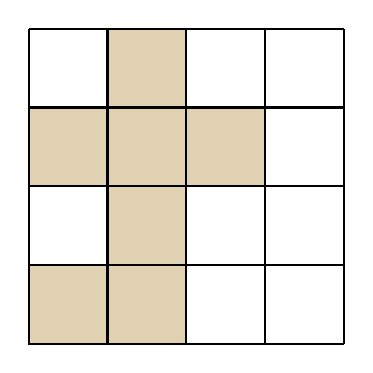
\begin{tikzpicture}
[thick]
\draw (0,0) grid (4,4);
\draw[fill=red!60!green!30!] (1,3) rectangle ++(1,1);
\draw[fill=red!60!green!30!] (1,2) rectangle ++(1,1);
\draw[fill=red!60!green!30!] (1,1) rectangle ++(1,1);
\draw[fill=red!60!green!30!] (1,0) rectangle ++(1,1);
\draw[fill=red!60!green!30!] (0,0) rectangle ++(1,1);
\draw[fill=red!60!green!30!] (0,2) rectangle ++(1,1);
\draw[fill=red!60!green!30!] (2,2) rectangle ++(1,1);
\end{tikzpicture}
\end{figure}
\end{flushleft}

\subsection{Depth Fist Search}

\begin{itemize}
\item To indicate a cell $G[x][y]$ is visited, we can change the value of this cell to a different value like 2.
\item This problem is to find the perimeter. For current cell $G[x][y]$, if it is surrounded by water, the perimeter will be 4. we check its four adjacent cells. If any one of them is also an island (either the value is 1 or 2), decrements the perimeter.
\item We recursively compute for any adjacent island that has not been visited.
\end{itemize}

\setcounter{lstlisting}{0}
\begin{lstlisting}[style=customc, caption={DFS}]
int islandPerimeter( vector<vector<int>>& grid )
{
    int R = static_cast<int>( grid.size() );
    int C = static_cast<int>( grid[0].size() );

    int ans = 0;

    for( int r = 0;  r < R; ++r )
    {
        for( int c = 0; c < C; ++c )
        {
            if( grid[r][c] == 1 )
            {
                dfs( grid, r, c,  ans );
                break;
            }
        }
    }

    return ans;
}

void dfs( vector<vector<int>>& G, int r, int c,  int& len )
{
    //set to 2 to indicate this island is seen before
    G[r][c] = 2;

    int R = static_cast<int>( G.size() );
    int C = static_cast<int>( G[0].size() );

    int dr[4] = {0, -1, 0, 1};
    int dc[4] = {1, 0, -1, 0};

    //If this island is sorrouding by water
    //the perimeter is 4
    //it will be changed if we find adjacent islands
    int p = 4;

    for( int i = 0; i < 4; ++i )
    {
        int nr = r + dr[i];
        int nc = c + dc[i];

        if( ( nr < 0 ) || ( nc < 0 ) || ( nr >= R ) || ( nc >= C ) )
        {
            continue;
        }

        if( G[nr][nc] == 2 )
        {
            //This is also an island
            //will not count the common edge
            --p;
            continue;
        }

        if( G[nr][nc] == 1 )
        {
            //This is also an island
            //will not count the common edge

            --p;
            dfs( G, nr, nc, len );
        }


    }

    len += p;
}
\end{lstlisting}
%\section{464 --- Can I Win}
In the \textbf{100 game}, two players take turns adding, to a running total, any integer from 1 to 10. The player who first causes the running total to reach or exceed 100 wins.

What if we change the game so that players cannot re-use integers?

For example, two players might take turns drawing from a common pool of numbers of $[1, 15]$ without replacement until they reach a total $\geq 100$.

Given an integer $x$ which is the maximum integer that the players can choose, and another integer $y$ which is the desired total, determine if the first player to move can force a win, assuming both players play optimally.

You can always assume that $x$ will not be larger than 20 and $y$ will not be larger than 300.

\paragraph{Example}

\begin{flushleft}
\textbf{Input}: $x = 10$ , $y = 11$

\textbf{Output}: \texttt{false}

\textbf{Explanation}: No matter which integer the first player choose, the first player will lose.

The first player can choose an integer from 1 up to 10.

If the first player choose 1, the second player can only choose integers from 2 up to 10.

The second player will win by choosing 10 and get a total equal to 11, which is equal or larger than $y$.

Same with other integers chosen by the first player, the second player will always win.
\end{flushleft}

\subsection{Depth First Search}

\setcounter{lstlisting}{0}
\begin{lstlisting}[style=customc, caption={Depth First Search}]
bool canIWin( int maxChoosableInteger, int desiredTotal )
{
    if( desiredTotal < 2 )
    {
        return true;
    }

    int sum = ( 1 + maxChoosableInteger ) * maxChoosableInteger / 2;

    if( sum < desiredTotal )
    {
        //no one can win
        return false;
    }

    if( sum == desiredTotal )
    {
        //only odd number first person can win
        return ( maxChoosableInteger & 1 );
    }

    unordered_map<int, unsigned char> memo;

    return dfs( maxChoosableInteger, desiredTotal, memo, 0 );
}

//the helper function to do depth first search
bool dfs( int x, int y, unordered_map<int, unsigned char>& memo, int state )
{
    auto it = memo.find( state );
    if( it != memo.end() )
    {
        return it->second == 1;
    }

    for( int i = 0; i < x; ++i )
    {
        //number i+1 is not selected
        if( !( state & ( 1 << i ) ) )
        {
            if( y <= ( i + 1 ) )
            {
                //since the first person will select (i+1)
                //if y < (i+1)
                //first person can win;
                memo.emplace( state, 1 );
                return true;
            }

            int next_state = ( state | ( 1 << i ) );

            if( !dfs( x, y - ( i + 1 ), memo, next_state ) )
            {
                memo.emplace( state, 1 );
                return true;
            }
        }
    }

    memo.emplace( state, 0 );
    return false;
}
\end{lstlisting}

%\section{465 --- Optimal Account Balancing}
A group of friends went on holiday and sometimes lent each other money. For example, Alice paid for Bill's lunch for \$10. Then later Chris gave Alice \$5 for a taxi ride. We can model each transaction as a tuple $(x, y, z)$ which means person $x$ gave person $y$ \$z. Assuming Alice, Bill, and Chris are person 0, 1, and 2 respectively (0, 1, 2 are the person's ID), the transactions can be represented as $ [[0, 1, 10], [2, 0, 5]] $.

Given a list of transactions between a group of people, $T$, return the minimum number of transactions required to settle the debt.

\paragraph{Note:}

\begin{itemize}
\item A transaction will be given as a tuple $ (x, y, z) $. Note that $x \neq y$ and $z > 0$.

\item Person's IDs may not be linear, e.g. we could have the persons 0, 1, 2 or we could also have the persons 0, 2, 6.
\end{itemize}

\paragraph{Example 1:}

\begin{flushleft}
\textbf{Input}:

$[[0,1,10], [2,0,5]]$

\textbf{Output}: 2

\textbf{Explanation}:

Person \#0 gave person \#1 \$10.

Person \#2 gave person \#0 \$5.


Two transactions are needed. One way to settle the debt is person \#1 pays person \#0 and \#2 \$5 each.
\end{flushleft}


\paragraph{Example 2:}

\begin{flushleft}
\textbf{Input}:

$ [[0,1,10], [1,0,1], [1,2,5], [2,0,5]] $

\textbf{Output}: 1

\textbf{Explanation}:
Person \#0 gave person \#1 \$10.
Person \#1 gave person \#0 \$1.
Person \#1 gave person \#2 \$5.
Person \#2 gave person \#0 \$5.

Therefore, person \#1 only need to give person \#0 \$4, and all debt is settled.
\end{flushleft}

\subsection{Depth First Search}
\begin{itemize}
\item Calculate each person's overall balance $B[i]$. $B[i]>0$ means person $i$ needs to pay $B[i]$ to other persons, while $B[i]<0$ person $i$ needs to get money from other people. 
\item We start from the first person with $B[0]$, skip all persons with $B[i]=0$ and try to find the first person that has opposite sign to $B[0]$, say, $B[j]$. We use $B[j]\gets B[j]+B[0]$ to clear $B[0]$.
\item From now on, $B[0]$ is cleared, and we recursively set other $B[k]$ to zero one by one until all $B[j]$ are zeros. At this time, update the global minimum transactions.
\end{itemize}

\setcounter{lstlisting}{0}
\begin{lstlisting}[style=customc, caption={DFS}]
int minTransfers( vector<vector<int>>& transactions )
{
    //get each person's overall balance
    unordered_map<int, int> m_bal;

    auto add_map = [&m_bal]( int id, int money )
    {
        auto it  = m_bal.find( id );
        if( it == m_bal.end() )
        {
            m_bal.emplace( id, money );
        }
        else
        {
            it->second += money;
        }
    };

    for( const auto& trans : transactions )
    {
        add_map( trans[0], -trans[2] );
        add_map( trans[1], +trans[2] );
    }

    //change to vector
    vector<int> v_bal;
    v_bal.reserve( m_bal.size() );

    for( const auto& p : m_bal )
    {
        if( p.second != 0 )
        {
            v_bal.push_back( p.second );
        }
    }

    int ans = INT_MAX;
    dfs( v_bal, 0, 0, ans );

    return ans;
}

void dfs( vector<int>& A, size_t start, int steps, int& ans )
{
    //skip person with zero balance
    while( ( start < A.size() ) && ( A[start] == 0 ) )
    {
        ++start;
    }

    if( start == A.size() )
    {
        //all persons are cleared
        //update minimum transactions
        ans = ( min )( ans, steps );
        return;
    }

    //try other persons
    auto next = start + 1;

    while( next < A.size() )
    {
        if( A[next] * A[start] < 0 )
        {
            //person next can help
            //clear person start
            int x = A[start];
            A[next] += x;

            //we seach from person (start+1)
            //increments the transactions
            dfs( A, start + 1, steps + 1, ans );

            //backtrack
            A[next] -= x;
        }
        ++next;
    }
}
\end{lstlisting}
%\section{466 --- Count The Repetitions}
Define $S = [s,n]$ as the string $S$ which consists of $n$ connected strings s. For example, \lstinline[language=C++, basicstyle=\small\ttfamily, keywordstyle=\bfseries\color{green!40!black}]|[abc, 3] = abcabcabc|.

On the other hand, we define that string $s_1$ can be obtained from string $s_2$ if we can remove some characters from $ s_2 $ such that it becomes $ s_1 $. For example, \lstinline[language=C++, basicstyle=\small\ttfamily, keywordstyle=\bfseries\color{green!40!black}]|"abc"| can be obtained from \lstinline[language=C++, basicstyle=\small\ttfamily, keywordstyle=\bfseries\color{green!40!black}]|"abdbec"| based on our definition, but it can not be obtained from \lstinline[language=C++, basicstyle=\small\ttfamily, keywordstyle=\bfseries\color{green!40!black}]|"acbbe"|.

You are given two non-empty strings $ s_1 $ and $ s_2 $ (each at most 100 characters long) and two integers $0 \leq n_1 \leq 10^6$ and $1 \leq n_2 \leq 10^6$. Now consider the strings $S_1$ and $S_2$, where $S_1=[s_1,n_1]$ and $S_2=[s_2,n_2]$. Find the maximum integer $M$ such that $[S_2,M]$ can be obtained from $S_1$.

\section{Example:}

\begin{flushleft}
\textbf{Input}:

$s_1=\texttt{acb}$, $n_1=4$

$s_2=\texttt{ab}$, $n_2=2$

\textbf{Return}: 2

\end{flushleft}

\subsection{Brute Force}
According to the question, we need to find $m$ such that $[S_2,m]$ is the largest subsequence (not substring) that can be found in $S_1$. Notice that $S_2$ is $s_2$ repeats for $n_2$ times and $S_1$ is $s_1$ repeats for $n_1$ times. Therefore, we can find the number of times which are how many $s_2$ repeats in $[s_1,n_1]$, denote as $x$. Then the number of times $S_2$ which is $[s_2,n_2]$ repeats in $S_1$ is $(x/n_2)$

\setcounter{algorithm}{0}
\begin{algorithm}[H]
\caption{Brute Force}
\begin{algorithmic}[1]
\Procedure{GetMaxRepetitions}{$s_1, L_1, n_1, s_2, L_2, n_2$}
\State $p := 0$ \Comment The current index in $s_2$ to be checked against $s_1$
\State $x := 0$ \Comment the number of times $s_2$ repeats in $S_1$
\For{$i:=1$ \textbf{to} $n_1$}
\For{$j:=0$ \textbf{to} $L_1-1$}
\If{$s_2[p] = s_1[j]$}
\State $p = p+1$
\EndIf
\algstore{466algo}
\end{algorithmic}
\end{algorithm}
\begin{algorithm}[H]
\begin{algorithmic}[1]
\algrestore{466algo}
\If{$p = L_2$} \Comment $s_2$ has completed one repetition 
\State $x \gets x + 1$ \Comment Repeat count increments
\State $p \gets 0$ \Comment Reset index in $s_2$ to zero
\EndIf
\EndFor
\EndFor
\State \Return $x/n_2$
\EndProcedure
\end{algorithmic}
\end{algorithm}

\subsection{Improved Scanning Strategy}
We need to scan $s_1$ for $n_1$ times. After completely scanning of $i$-th $s_1$ block, we will have

\begin{itemize}
\item The accumulative count of $s_2$ repeated so far.
\item The next position $p$ in $s_2$. We will search $s_2[p]$ first in the $(i+1)$th $s_1$ block.
\end{itemize}

For example, Suppose $s_1=\texttt{abc}$, $s_2=\texttt{bac}$, after scanning the first $s_1$ block, we have found $s_2[0]$. We will look for $s_2[1]$ in the second $s_1$ block. Therefore $p=1$. The values for $p$ is in the range $[0, \lvert s_2\rvert]$. Therefore, by the \textbf{Pigeonhole principle}, we must have two same $p$ after scanning ($\lvert s_2\rvert + 1$) $s_1$ blocks.

The following picture shows how $p$ and count of $s_2$ are updated where we have 

\begin{itemize}
\item $s_1=\texttt{abaacdbac}$ and $n_1=100$
\item $s_2=\texttt{adcbd}$ and $n_2=4$
\end{itemize}

\begin{figure}[H]
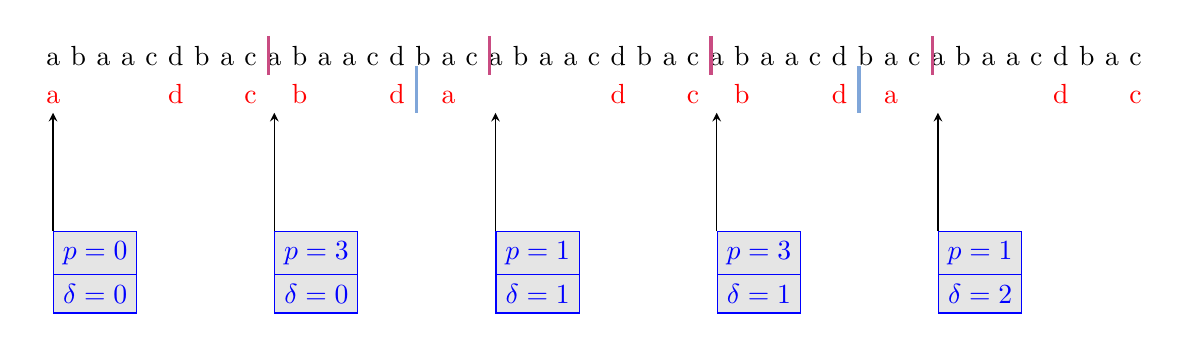
\begin{tikzpicture}
[my/.style={draw, rectangle split, rectangle split parts=2, color=blue, fill=gray!20!, minimum height=1cm}]
\matrix[every node/.style={anchor=base}, column sep=-1mm]
{
\node(a0){a};& \node{b}; & \node{a};& \node{a};& \node{c};& \node{d};& \node{b};& \node{a};& \node(t0){c}; & \node(a1){a};& \node{b}; & \node{a};& \node{a};& \node{c};& \node{d};& \node{b};& \node{a};& \node(t1){c}; 
& \node(a2){a};& \node{b}; & \node{a};& \node{a};& \node{c};& \node{d};& \node{b};& \node{a};& \node(t2){c};

& \node(a3){a};& \node{b}; & \node{a};& \node{a};& \node{c};& \node{d};& \node{b};& \node{a};& \node(t3){c};

& \node(a4){a};& \node{b}; & \node{a};& \node{a};& \node{c};& \node{d};& \node{b};& \node{a};& \node(t4){c};

\\
\node(b0){\textcolor{red}{a}}; & \node{}; & \node{}; & \node{};& \node{};& \node{\textcolor{red}{d}}; & \node{};& \node{};& \node{\textcolor{red}{c}}; & \node(b1){}; & \node{\textcolor{red}{b}}; & \node{}; & \node{};& \node{};& \node(e0){\textcolor{red}{d}}; & \node{};& \node{\textcolor{red}{a}};& \node{};\node{}; 
& \node(b2){}; & \node{}; & \node{};& \node{};& \node{}; & \node{\textcolor{red}{d}};& \node{};& \node{}; & \node{\textcolor{red}{c}}; 

& \node(b3){}; & \node{\textcolor{red}{b}}; & \node{};& \node{};& \node{}; & \node(e1){\textcolor{red}{d}};& \node{};& \node{\textcolor{red}{a}}; & \node{};

& \node(b4){}; & \node{}; & \node{};& \node{};& \node{}; & \node{\textcolor{red}{d}};& \node{};& \node{}; & \node{\textcolor{red}{c}}; \\
};

\node[my](i0) [below=1.5cm of b0.south, anchor=north west] {$p=0$\nodepart{two}$\delta=0$};
\draw[>=stealth, ->] (i0.north west) -- (b0.south);

\node[my](i1) [below=1.5cm of b1.south, anchor=north west] {$p=3$\nodepart{two}$\delta=0$};
\draw[>=stealth, ->] (i1.north west) -- (b1.south);

\node[my](i2) [below=1.5cm of b2.south, anchor=north west] {$p=1$\nodepart{two}$\delta=1$};
\draw[>=stealth, ->] (i2.north west) -- (b2.south);

\node[my](i3) [below=1.5cm of b3.south, anchor=north west] {$p=3$\nodepart{two}$\delta=1$};
\draw[>=stealth, ->] (i3.north west) -- (b3.south);

\node[my](i4) [below=1.5cm of b4.south, anchor=north west] {$p=1$\nodepart{two}$\delta=2$};
\draw[>=stealth, ->] (i4.north west) -- (b4.south);

\draw[very thick, blue!30!red!70!] ($(t0.north east) + (0.25mm, 1mm)$) -- ($(t0.south east) + (0.25mm, 0)$);
\draw[very thick, blue!30!red!70!] ($(t1.north east) + (0.25mm, 1mm)$) -- ($(t1.south east) + (0.25mm, 0)$);

\draw[very thick, blue!30!red!70!] ($(t2.north east) + (0.25mm, 1mm)$) -- ($(t2.south east) + (0.25mm, 0)$);

\draw[very thick, blue!30!red!70!] ($(t3.north east) + (0.25mm, 1mm)$) -- ($(t3.south east) + (0.25mm, 0)$);
\draw[very thick, green!30!blue!50!] ($(e0.north east) + (0.25mm, 1mm)$) -- ($(e0.south east) + (0.25mm, 0)$);
\draw[very thick, green!30!blue!50!] ($(e1.north east) + (0.25mm, 1mm)$) -- ($(e1.south east) + (0.25mm, 0)$);
\end{tikzpicture}
\end{figure}

\paragraph{Outline}

\begin{itemize}
\item Maintain two arrays (or two hash maps to improve efficiency) $a$ and $b$. Both of them have the size equal to $\lvert s_2\rvert+1$ as mentioned before.
\item $a$ records $p$ while $b$ saves the accumulative count of $s_2$ at the start of each $s_1$ block in $S_1$.
\item Loop over the $n_1$ blocks of $s_1$. At current $i$th $s_1$ block, we check if a repetition of $p$ can be found in $a$. That is, if there exits a $k$ such that $a[k] = p$ and $0\leq k\leq (i-1)$.
\item If we find a $a[k]=p$, it means the a complete pattern is across from $k+1$th to $(i)$th block (the pattern restarts after $k$ th block). Hence, the pattern's \textbf{length} is $i-k$ blocks. Take the picture above as the example, we find $p=3$ at 2nd $s_1$ block and 4rd block. The pattern spans 2 blocks (3rd and 4th block).
\item From $(k+1)$th block to $n_1-1$th block, there are $n_1-k-1$ blocks. By considering the length of one pattern, we would have $q= \lfloor (n_1-k-1)/(i-k)\rfloor$ patterns.
\item In each pattern, $s_2$ appears $b[i] - b[k]$ times. As a result, the total counts of $s_2$ in all repeated patterns are $q\times (b[i]-b[k])$.  Take the picture above as the example, there are only one $s_2$ subsequence from 3rd block to 4th block.
\item If $(n_1-k-1)$ does not divided by $i-k$, the remainder $r$ is number of blocks after the whole patterns. These $r$ blocks do not contain the pattern. The number of $s_2$ in these $r$ blocks are $\delta[n_1-1] - \delta[k+(i-k)\times q] = \delta[k+(i-k)\times q + r] - \delta[k+(i-k)\times q]$. Since the pattern repeats for $q$ times, the increments of the number of $s_2$ also repeats. Then we get $\delta[k+(i-k)\times q + r] - \delta[k+(i-k)\times q] = \delta[k+r]-\delta[k]$. 
\item We also need to know how many $s_2$ exist before the pattern starts. This is indeed is $b[k]$.
\item Edge case: If no repeating pattern is found, this implies $n_1 < \lvert s_2\rvert+1$ by the above analysis. In this case, the counts of $s_2$ in $s_1$ is $b[n_1-1]/(n_2)$.
\end{itemize}

\begin{algorithm}[H]
\caption{Improved Scanning Strategy}
\begin{algorithmic}[1]
\Procedure{GetMaxRepetitions}{$s_1$, $L_1$, $n_1$, $s_2$, $L_2$, $n_2$}
\State $\star$ Initialize an array $a$ with length $L_1+1$ to store index of $s_2$ at start of each $s_1$ block
\State $\star$ Initialize an array $b$ with length $L_1+1$ to store count of $s_2$ at start of each $s_1$ block
\State $p := 0$
\State $\delta := 0$
\For{$i:=0$ \textbf{to} $n_1-1$} \label{466Loop1}
\For{$j:=0$ \textbf{to} $L_2-1$} \label{466Loop2}
\If{$s_1[i] = s_2[j]$}
\State $p\gets p+1$
\EndIf
\algstore{466algo}
\end{algorithmic}
\end{algorithm}
\begin{algorithm}[H]
\begin{algorithmic}[1]
\algrestore{466algo}
\If{$p = L_2$}
\State $p \gets 0$
\State $\delta \gets \delta + 1$
\EndIf
\EndFor \Comment End[\ref{466Loop2}]
\State $b[i] \gets \delta$
\State $a[i] \gets p$
\For{$k:=0$ \textbf{to} $i-1$} \label{466Loop3}
\If{$p = a[k]$}
\State $\alpha := i - k$ \Comment The interval of pattern
\State $q := (n_1-k)/(\alpha)$ \Comment The repeat times of pattern
\State $r := (n_1-k) - q \times \alpha$ \Comment The blocks does not contain the pattern
\State $z := (b[i]-b[k])\times q$ \Comment The total $s_2$ in all patterns
\State $\hat{z}:=(b[k+r] - b[k])$ \Comment total $s_2$ after the patterns
\State $p:=b[k]$ \Comment total $s_2$ before the patterns.
\State $x:=(z+\hat{z}+p) / n_2$ \Comment Total $S_2$ in $S_1$
\State \Return $x$
\EndIf
\EndFor \Comment End line [\ref{466Loop3}]
\EndFor \Comment End line [\ref{466Loop1}]
\State $\ast$ If no repeating pattern is found, the whole count of $s_2$ divided by $n_2$ is the result
\State \Return $b[n_1-1]/n_2$
\EndProcedure
\end{algorithmic}
\end{algorithm}

\setcounter{lstlisting}{0}
\begin{lstlisting}[style=customc, caption={Find Repeat Pattern}]
int getMaxRepetitions( string s1, int n1, string s2, int n2 ) {

    unordered_map<int, int> p_dict; //position
    unordered_map<int, int> d_dict; //accumulate counts

    int s2_i = 0; //the index of s2 in the next s1 block
    int s2_counts = 0; //count of s2 so far

    int L1 = static_cast< int >( s1.size() );
    int L2 = static_cast< int >( s2.size() );

    for( int block = 1; block <= n1; ++block )
    {
        for( int s1_i = 0; s1_i < L1; ++s1_i )
        {
            if( s2[s2_i] == s1[s1_i] )
            {
                ++s2_i;
            }

            //one s2 has been scanned
            if( s2_i == L2 )
            {
                s2_i = 0;
                ++s2_counts;
            }
        }
        //find if this position
        //has appeared before
        auto it = p_dict.find( s2_i );
        if( it == p_dict.end() )
        {
            //not found
            //we have not found repetition pattern

            //link current scanned index in s2
            //and the block
            p_dict.emplace( s2_i, block );

            //link current block and number of s2 have been
            //found
            d_dict.emplace( block, s2_counts );
        }
        else
        {
            int start_block = it->second;

            //how many blocks that the pattern across
            //the pattern is across [start_block+1, block]
            int num_blocks = block - start_block;

            //how many patterns we can find from start_block to the end
            int num_patterns = ( n1 - start_block ) / num_blocks;

            //how many blocks that cannot support a whole pattern after
            int rem_blocks = ( n1 - start_block ) - num_blocks * num_patterns;

            // now we need to count number of s2 from the pattern

            //get how many s2 are there before the pattern start
            int num_s2_before_pattern = d_dict[start_block];

            //number of s2 in all patterns
            int num_s2_in_pattern = ( s2_counts - d_dict[start_block] ) * num_patterns;

            //number of s2 after the pattern
            //this should be d_dict[n1] - d_dict[block]
            //but right now d_dict[n1] is not available
            //however, we know that n1=start_block + num_blocks + rem_blocks;
            // block = start_block + num_blocks;
            //the increments of s2 inside these blocks will also repeat
            int num_s2_after_pattern = d_dict[start_block + rem_blocks] - d_dict[start_block];

            return ( num_s2_before_pattern + num_s2_in_pattern + num_s2_after_pattern ) / n2;
        };

    }

    //no repetition can be found
    //only returns the recorded total number of s2
    //divided by n2
    return d_dict[n1] / n2;
}
\end{lstlisting}


%\section{467 --- Unique Substrings in Wraparound String}
Consider the string $s$ to be the infinite wraparound string of \texttt{abcdefghijklmnopqrstuvwxyz}, so $s$ will look like this:  $\ldots \texttt{zabcdefghijklmnopqrstuvwxyzabcdefghijklmnopqrstuvwxyzabcd} \ldots$.

Now we have another string $p$. Your job is to find out how many unique non-empty substrings of $p$ are present in $s$. In particular, your input is the string $p$ and you need to output the number of different non-empty substrings of $p$ in the string $s$.

\paragraph{Note:} 
\begin{itemize}
\item $p$ consists of only lowercase English letters and the size of $p$ might be over 10000.
\end{itemize}

\paragraph{Example 1:}
\begin{flushleft}
\textbf{Input}: \texttt{a}

\textbf{Output}: 1

\textbf{Explanation}: Only the substring a of string \texttt{a} is in the string.

\end{flushleft}


\paragraph{Example 2:}
\begin{flushleft}

\textbf{Input}: \texttt{cac}

\textbf{Output}: 2

\textbf{Explanation}: There are two substrings \texttt{a}, \texttt{c} of string \texttt{cac} in the string \texttt{s}.


\end{flushleft}

\paragraph{Example 3:}
\begin{flushleft}
\textbf{Input}: \texttt{zab}

\textbf{Output}: 6

\textbf{Explanation}: There are six substrings \texttt{z}, \texttt{a}, \texttt{b}, \texttt{za}, \texttt{ab}, \texttt{zab} of string \texttt{zab} in the string $s$.
\end{flushleft}

\subsection{Dynamic Programming}
The idea is, if we know the max number of unique substrings in $p$ ends with $a, b, \ldots, z$, then add them together will be the answer. 

\begin{itemize}
\item The max number of unique substring ends with a letter equals to the length of max contiguous substring ends with that letter. For example \texttt{abcd}, the max number of unique substring ends with $d$ is 4, apparently they are \texttt{abcd}, \texttt{bcd}, \texttt{cd} and \texttt{d}.
\item If there are overlapping, we only need to consider the longest one because it covers all the possible substrings. For example: \texttt{abcdbcd}, the max number of unique substring ends with $d$ is 4 and all substrings formed by the 2nd \texttt{bcd} part are covered in the 4 substrings already.
\item No matter how long is a contiguous substring in $p$, it must be in $s$ because $s$ is infinite.
\end{itemize}

\setcounter{lstlisting}{0}
\begin{lstlisting}[style=customc, caption={Dynamic Programming}]
int findSubstringInWraproundString( string p )
{
	//the maximum contiguous substring length 
	//ending in each letter.
    int count[26] = {0};

	//current contiguous substring length
    int x = 1;

    for( size_t i = 0; i < p.size(); ++i )
    {
        int ci = p[i] - 'a';

        //check the contiguous substring length
        //ending with p[i]
        if( i > 0 )
        {
            int last = p[i - 1] - 'a';
            int next = ( ( last + 1 ) % 26 );

            if( next == ci )
            {
				//last letter and current letter
				//is contiguous
				//increments the contiguous substring length
				//ending in current letter
                ++x; 
            }
            else
            {
				//reset the contiguous substring length
				//ending in current letter
                x = 1;
            }
        }

        count[ci] = ( max )( count[ci], x );
    }

    //the total of maximum length ending in each letter
    //is the answer
    int ans = 0;

    for( int i = 0; i < 26; ++i )
    {
        ans += count[i];
    }

    return ans;
}
\end{lstlisting}
%\section{468 --- Validate IP Address}
Write a function to check whether an input string is a valid IPv4 address or IPv6 address or neither.

IPv4 addresses are canonically represented in dot-decimal notation, which consists of four decimal numbers, each ranging from 0 to 255, separated by dots, e.g.,172.16.254.1;

Besides, leading zeros in the IPv4 is invalid. For example, the address 172.16.254.01 is invalid.

IPv6 addresses are represented as eight groups of four hexadecimal digits, each group representing 16 bits. The groups are separated by colons. For example, the address 2001:0db8:85a3:0000:0000:8a2e:0370:7334 is a valid one. Also, we could omit some leading zeros among four hexadecimal digits and some low-case characters in the address to upper-case ones, so 2001:db8:85a3:0:0:8A2E:0370:7334 is also a valid IPv6 address(Omit leading zeros and using upper cases).

However, we don't replace a consecutive group of zero value with a single empty group using two consecutive colons (::) to pursue simplicity. For example, 2001:0db8:85a3::8A2E:0370:7334 is an invalid IPv6 address.

Besides, extra leading zeros in the IPv6 is also invalid. For example, the address 02001:0db8:85a3:0000:0000:8a2e:0370:7334 is invalid.

Note: You may assume there is no extra space or special characters in the input string.

\paragraph{Example 1:}

\begin{flushleft}
\textbf{Input}: 172.16.254.1

\textbf{Output}: IPv4

\textbf{Explanation}: This is a valid IPv4 address, return IPv4.

\end{flushleft}

\paragraph{Example 2:}

\begin{flushleft}
\textbf{Input}: 2001:0db8:85a3:0:0:8A2E:0370:7334

\textbf{Output}: IPv6

\textbf{Explanation}: This is a valid IPv6 address, return IPv6.
\end{flushleft}

\paragraph{Example 3:}

\begin{flushleft}
\textbf{Input}: 256.256.256.256

\textbf{Output}: Neither

\textbf{Explanation}: This is neither a IPv4 address nor a IPv6 address.
\end{flushleft}

\subsection{String Processing}
\setcounter{lstlisting}{0}
\begin{lstlisting}[style=customc, caption={String Processing}]
string validIPAddress( string IP )
{

    if( IP.find( '.' ) != string::npos )
    {
        if( check_ip4( IP.c_str(), IP.size() ) )
        {
            return "IPv4";
        }

    }
    else if( IP.find( ':' ) != string::npos )
    {
        if( check_ip6( IP.c_str(), IP.size() ) )
        {
            return "IPv6";
        }

    }

    return "Neither";

}

bool check_ip4( const char* s, size_t len )
{
    int blocks = 1;

    size_t start = 0;

    int num = 0;

    for( size_t i = 0; i < len; ++i )
    {
        if( ( s[i] >= '0' ) && ( s[i] <= '9' ) )
        {
            num  = num * 10 + ( s[i] - '0' );

            //the ip block is larger than 255
            if( num > 255 )
            {
                return false;
            }

            if( i == len - 1 )
            {
                //check the validity of last block
                if( num )
                {
                    if( s[start] == '0' )
                    {
                        //leading zeros for non-zero values
                        return false;
                    }
                }
                else
                {
                    if( i - start >= 1 )
                    {
                        //two or more consecutive zeros
                        //for num = 0
                        return false;
                    }
                }

            }
        }
        else if( s[i] == '.' )
        {
            if( i == len - 1 )
            {
                //ending with dot is not allowed
                return false;
            }

            if( num != 0 )
            {
                if( s[start] == '0' )
                {
                    //leading zeros for non-zero values
                    return false;
                }
            }
            else
            {
                if( i - start >= 2 )
                {
                    //two or more consecutive zeros
                    //for num = 0

                    return false;
                }
            }

            if( i == start )
            {
                //two consecutive dots
                return false;
            }

            //set next block's start position
            start = i + 1;

            //reset the number to zero
            num = 0;

            //increments the blocks
            ++blocks;

            if( blocks > 4 )
            {
                //only 4 blocks are allowed
                return false;
            }
        }
        else
        {
            //other characters are not allowed
            return false;
        }
    }

    //only 4 blocks are allowed.
    //We may get less than 4 blocks
    return blocks == 4;
}

bool check_ip6( const char* s, size_t len )
{
    int blocks = 1;

    size_t start = 0;

    int block_len = 0;

    for( size_t i = 0; i < len; ++i )
    {
        if( is_hexnum( s[i] ) )
        {
            ++block_len;

            if( block_len > 4 )
            {
                //each block can only have 4 valid characters
                return false;
            }
        }
        else if( s[i] == ':' )
        {
            if( ( i == start ) || ( i == len - 1 ) )
            {
                //either two consecutive colons
                //or ending with colon
                return false;
            }

            //set the start position of next block
            start = i + 1;

            ++blocks;

            if( blocks > 8 )
            {
                //only 8 blocks are allowed
                return false;
            }

            //reset counter of each block's characters
            block_len = 0;
        }
        else
        {
            return false;
        }
    }

    return blocks == 8;
}

//helper function to
//determine if a character belongs
//to a hex number
bool is_hexnum( char c )
{
    if( ( c >= '0' ) && ( c <= '9' ) )
    {
        return true;
    }

    if( ( c >= 'A' ) && ( c <= 'F' ) )
    {
        return true;
    }

    if( ( c >= 'a' ) && ( c <= 'f' ) )
    {
        return true;
    }

    return false;
}

\end{lstlisting}

%\section{469 --- Convex Polygon}
Given a list of points that form a polygon when joined sequentially, find if this polygon is convex (Convex polygon definition).


\paragraph{Note:}

\begin{itemize}
\item There are at least 3 and at most 10,000 points.
\item Coordinates are in the range $-10,000$ to 10,000.
\item You may assume the polygon formed by given points is always a simple polygon (Simple polygon definition). In other words, we ensure that exactly two edges intersect at each vertex, and that edges otherwise don't intersect each other.

\end{itemize}

\paragraph{Example 1:}

\begin{flushleft}
\textbf{Input}: [[0,0],[0,1],[1,1],[1,0]]

\begin{figure}[H]
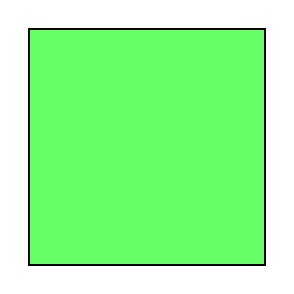
\begin{tikzpicture}[thick]
\draw[fill=green!60!white!] (0,0) rectangle ++(3,3);
\end{tikzpicture}
\end{figure}


\textbf{Output}: \texttt{True}
\end{flushleft}


\paragraph{Example 2:}

\textbf{Input}: $[[0,0],[0,10],[10,10],[10,0],[5,5]]$

\textbf{Output}: \texttt{False}

\textbf{Explanation}:

\begin{figure}[H]

\begin{tikzpicture}[thick]
\draw[fill=red!60!white] (0,0) -- (0,3) -- (3,3) --(3,0) -- (1.5,1.5) -- (0,0);
\end{tikzpicture}
\end{figure}

\subsection{Normal Vector}





%\section{470 --- Implement Rand10() Using Rand7()}
Given a function \texttt{rand7} which generates a uniform random integer in the range 1 to 7, write a function \texttt{rand10} which generates a uniform random integer in the range 1 to 10.

\paragraph{Example 1:}

\begin{flushleft}
\textbf{Input}: 1

\textbf{Output}: [7]
\end{flushleft}

\paragraph{Example 2:}

\begin{flushleft}
\textbf{Input}: 2

\textbf{Output}: [8,4]
\end{flushleft}

\paragraph{Example 3:}

\begin{flushleft}
\textbf{Input}: 3

\textbf{Output}: [8,1,10]
\end{flushleft}
 

\paragraph{Note:}

\begin{itemize}
\item \texttt{rand7} is predefined.
\item Each testcase has one argument: $n$, the number of times that rand10 is called.
\end{itemize}
 

\paragraph{Follow up:}

\begin{itemize}
\item What is the expected value for the number of calls to rand7() function?
\item Could you minimize the number of calls to rand7()?
\end{itemize}

\subsection{Rejection Sampling}

This solution is based upon \textbf{Rejection Sampling}. The main idea is when generating a number in the desired range, output that number immediately. If the number is out of the desired range, reject it and re-sample again. As each number in the desired range has the same probability of being chosen, a uniform distribution is produced.

Obviously, \texttt{rand7()} function has to be run at least twice, as there are not enough numbers in the range of 1 to 10. Running \texttt{rand7} twice can generate integers from 1 to 49 uniformly. Why?

\[
\begin{bmatrix}
 & \mathit{1} & \mathit{2} & \mathit{3} & \mathit{4} & \mathit{5} & \mathit{6} & \mathit{7} \\
\mathit{1} & 1 & 2 & 3 & 4 & 5 & 6 & 7 \\ 
\mathit{2} & 8 & 9 & 10 & 1 & 2 & 3 & 4 \\
\mathit{3} & 5 & 6 & 7 & 8 & 9 & 10 & 1\\
\mathit{4} & 2 & 3 & 4 & 5 & 6 & 7 & 8 \\
\mathit{5} & 9 & 10 & 1 & 2 & 3 & 4 & 5 \\
\mathit{6} & 6 & 7 & 8 & 9 & 10 & \ast & \ast \\
\mathit{7} & \ast & \ast & \ast & \ast & \ast & \ast & \ast \\
\end{bmatrix}
\]

As this table shows, Calling \texttt{rand7} twice will get row and column index that corresponds to a unique position in the table above. If a randomly chosen number from the table above hit a number, return that number immediately. If hit a $\ast$ , repeat the process again until hit a number.

Since 49 is not a multiple of 10, reject sampling needs to be used to generate the number from the desired range which is $[1, 40]$. Therefore, if the number is in the range $[1, 40]$, return it immediately, otherwise, reject it and re-sample again.

The expected value for the number of calls to \texttt{rand7} can be computed as follows
\begin{itemize}
\item Running 2 times and then get the number in range $[1, 40]$, the probability is $\dfrac{40}{49}$
\item Running 4 times and then get the number in range $[1, 40]$. This means the first round only get number in $[41,49]$, therefore, the jointed probability is $\dfrac{9}{49}\times\dfrac{40}{49}$
\item  依次类推 $\ldots$  
\end{itemize}

\begin{align*}
E &= 2\times \dfrac{40}{49} + 4\times \dfrac{9}{40} \times \dfrac{40}{49} + 6\times \left(\dfrac{9}{40}\right)^{2} \times \dfrac{40}{49} +\ldots \\
  &= \sum\limits_{i=1}^{\infty}\left(\dfrac{9}{40}\right)^{i-1}\left(\dfrac{40}{49}\right) \\
  & = \dfrac{80}{49\times \left(1-\dfrac{9}{49}\right)^2} = 2.45
\end{align*}

\setcounter{algorithm}{0}
\begin{algorithm}[H]
\caption{Rejection Sampling}
\begin{algorithmic}[1]
\Procedure{Rand10}{}
\Repeat
\State $\ast$ To generate from range $[1,40]$, we have $(r-1)\times 7 +c$
\State $r \gets$ \Call{rand7}{}
\State $r\gets R-1$
\State $c \gets$ \Call{rand7}{}
\State $x \gets r\times 7 + c$
\Until{$x \leq 40$}
\State \Return $1+(x-1)\bmod 10$
\EndProcedure
\end{algorithmic}
\end{algorithm}


\setcounter{lstlisting}{0}
\begin{lstlisting}[style=customc, caption={Rejection Sampling}]
int rand10()
{
    //using rand7 generate
    //row and column respectively
    //To make the loop start
    //set x to a large value
    int x = 49;

    //we need to select sample between [1,40]
    //because 40 is multiple of 10
    while( x > 40 )
    {
        int r = rand7();
        int c = rand7();

        x = ( r - 1 ) * 7 + c;
    }

    //generate number between [1,10]
    return 1 + ( x - 1 ) % 10;
}
\end{lstlisting}


\subsection{Out-of-range Sample Utilization}
Here are a total of \textbf{2.45} calls to \textbf{rand7()} on average when using the first approach. However, the average number of calls to rand7() can be improved by about 10\%.

The idea is that the \textbf{out-of-range} samples should not be disregarded, but instead use them to increase the chances of finding an in-range sample on the successive call to \textbf{rand7}.

The algorithm process is listed as below:

\begin{itemize}
\item Starting by generating a random integer in the range 1 to 49 using the table same as in rejection sampling. 
\item In the event that a generated number is outside the desired range $[1,40]$, it is equally likely that each number in $[41,49]$ would be chosen. In other words, integers in the range of 1 to 9 can be obtained uniformly. 
\item Now, run \texttt{rand7} again to obtain integers in the range $[1,63]$ uniformly. Apply rejection sampling where the desired range is $[1,60]$ since 60 is the multiple of 10. 
\item If the generated number is in the desired range $[1,60]$, return it. 
\item Otherwise, at least integers of 1 to 3 can be obtained uniformly. Run \texttt{rand7} again to obtain integers in the range $[1,21]$ uniformly. The desired range is $[1,20]$, and in the unlikely event when a 21 is obtained, reject it and repeat the entire process again.
\item 由于在上述 range $[1,21]$,只有一个数out side of range,即21,已经到达极限了,所以可以终止上述过程了。
\end{itemize}

The expected value for the number of calls to \texttt{rand7} can be computed as follows
\begin{align*}
E &= 2\times \dfrac{40}{49} + 3\times \dfrac{9}{40} \times \dfrac{60}{63} + 4\times \dfrac{9}{40} \times \dfrac{60}{63} \times \dfrac{20}{21}  \\
  &+ \dfrac{9}{40} \times \dfrac{60}{63} \times \dfrac{1}{20} \times \left(6\times \dfrac{40}{49} + 7 \times \dfrac{9}{40} \times \dfrac{60}{63} + 8 \times \times \dfrac{9}{40} \times \dfrac{60}{63} \times \dfrac{20}{21}\right) \\
  &+ \left(\dfrac{9}{40} \times \dfrac{60}{63} \times \dfrac{1}{20}\right)^2\times \left(10\times \dfrac{40}{49} + 11 \times \dfrac{9}{40} \times \dfrac{60}{63} + 12 \times \times \dfrac{9}{40} \times \dfrac{60}{63} \times \dfrac{20}{21}\right) \\
  &+ \ldots \\
  &= 2.2123 
\end{align*}

\subsubsection{Algorithm}
\begin{algorithm}[H]
\caption{Rejection Sampling With Out-of-range Utilization}
\begin{algorithmic}[1]
\Procedure{Rand10}{}
\Loop
\State $\ast$ Generate number in $[1,49]$
\State $r \gets $ \Call{rand7}{}
\State $c \gets $ \Call{rand7}{}
\State $x \gets (r-1)\times 7 + c$
\If{$x \leq 40$}
\State \Return $1+(x-1)\bmod 10$ \Comment Return when in range $[1,40]$
\EndIf
\State $\ast$ Otherwise, generate $[1,63]$ for number in $[41,49]$
\State $x\gets x - 40$ \Comment $x\in[1,9]$
\State $\ast$ Generate another number in $[1,7]$
\State $y \gets $ \Call{rand7}{}
\State $x \gets (x-1)\times 7 + y$  \Comment $x\in [1, 63]$
\If{$x \leq 60$}
\State \Return $1+(x-1)\bmod 10$ \Comment Return when in range $[1,60]$
\EndIf
\State $\ast$ Otherwise, generate $[1,21]$ for number in $[1,3]$
\State $x\gets x - 60$ \Comment $x \in [1,3]$
\State $\ast$ Generate another number in $[1,7]$
\State $y \gets $ \Call{rand7}{}
\State $x \gets (x-1)\times 7 + y$  \Comment $x\in [1, 21]$
\If{$x \leq 20$}
\State \Return $1+(x-1)\bmod 10$
\EndIf
\EndLoop
\EndProcedure
\end{algorithmic}
\end{algorithm}

\setcounter{lstlisting}{0}
\begin{lstlisting}[style=customc, caption={Out-of-range Utilization}]
// The rand7() API is already defined for you.
// int rand7();
// @return a random integer in the range 1 to 7

int rand10()
{
    while( true )
    {
        //generate [1,49]
        int r = rand7();
        int c = rand7();

        int x = ( r - 1 ) * 7 + c;

        if( x <= 40 )
        {
            //40 is multiple of 10
            return 1 + ( x - 1 ) % 10;
        }

        //utilize out-of-range samples
        //generate [1,63] for [41,49]
        x -= 40;
        int y = rand7();

        x = ( x - 1 ) * 7 + y;

        if( x <= 60 )
        {
            //60 is multiple of 10
            return 1 + ( x - 1 ) % 10;
        }

        //utilize out-of-range samples
        //generate [1,21] for [1,3]
        x -= 60;
        y = rand7();

        x = ( x - 1 ) * 7 + y;

        if( x <= 20 )
        {
            //20 is multiple of 10
            return 1 + ( x - 1 ) % 10;
        }
        //since only 21 is the out-of-range sample
        //no need to further the steps before
        //start the process again
    }

    //this will never get
    //only for compilation
    return 0;
}

\end{lstlisting}
%\section{471 --- Encode String with Shortest Length}
\textcolor{red}{\large Locked}


Given a non-empty string $s$, encode the string such that its encoded length is the shortest.

The encoding rule is: $k[t]$, where the $t$ inside the square brackets is being repeated exactly $k$ times.

\paragraph{Note:}
\begin{itemize}
\item $k$ will be a positive integer and encoded string will not be empty or have extra space.
\item You may assume that the input string contains only lowercase English letters. The string's length is at most 160.
\item If an encoding process does not make the string shorter, then do not encode it. If there are several solutions, return any of them is fine.
\end{itemize}

\paragraph{Example 1:}

\begin{flushleft}
\textbf{Input}: \texttt{aaa}

\textbf{Output}: \texttt{aaa}

\textbf{Explanation}: There is no way to encode it such that it is shorter than the input string, so we do not encode it.

\end{flushleft}
\paragraph{Example 2:}

\begin{flushleft}
\textbf{Input}: \texttt{aaaaa}

\textbf{Output}: 5[\texttt{a}]

\textbf{Explanation}: 5[\texttt{a}] is shorter than \texttt{aaaaa} by 1 character.

\end{flushleft}

\paragraph{Example 3:}

\begin{flushleft}

\textbf{Input}: \texttt{aaaaaaaaaa}

\textbf{Output}: 10[\texttt{a}]

\textbf{Explanation}: \texttt{a}9[\texttt{a}] or 9[\texttt{a}]\texttt{a} are also valid solutions, both of them have the same length  5, which is the same as 10[\texttt{a}].

\end{flushleft}
\paragraph{Example 4:}

\begin{flushleft}

\textbf{Input}: \texttt{aabcaabcd}

\textbf{Output}: 2[\texttt{aabc}]d

\textbf{Explanation}: \texttt{aabc} occurs twice, so one answer can be 2[\texttt{aabc}]d.

\end{flushleft}
\paragraph{Example 5:}

\begin{flushleft}
\textbf{Input}: \texttt{abbbabbbcabbbabbbc}

\textbf{Output}: 2[2[\texttt{abbb}]\texttt{c}]

\textbf{Explanation}: \texttt{abbbabbbc} occurs twice, but \texttt{abbbabbbc} can also be encoded to 2[\texttt{abbb}]\texttt{c}, so one answer can be 2[2[\texttt{abbb}]\texttt{c}].
\end{flushleft}


\subsection{Dynamic Programming}
Suppose $F[i][j]$ is the minimum encoded string for $s[i,j]$. 

\begin{enumerate}
\item Break $s[i,j]$ in each index $x\in [i+1, j-1]$, we can get $F[i][x]$ and $F[x+1][j]$. 
\item Get the total length of $F[i][x]$ and $F[x+1][j]$, compared to and update the global minimum length when possible. 
\item We still also need to check if $s[i,j]$ can be directly represented by a minimum encoded string. If this is possible, we may need to compare this encoded string length to string acquired in the step 2. (Note: in this step, suppose the $s[i][j]$ has a repeatable string $z$, we may also need $z$'s minimum encoded string not $z$ by itself)
\end{enumerate}

\setcounter{lstlisting}{0}
\begin{lstlisting}[style=customc, caption={Dynamic Programming}]
string encode( string s )
{

    //F[i][j] is the minimum encoded string for s[i,j];

    vector<vector<string>> F( s.size(), vector<string>( s.size() ) );

    //fill size 1

    for( size_t i = 0; i < s.size(); ++i )
    {
        F[i][i].push_back( s[i] );
    }

    //file size 2
    for( size_t i = 0; i < s.size() - 1; ++i )
    {
        F[i][i + 1].push_back( s[i] );
        F[i][i + 1].push_back( s[i + 1] );
    }

    for( size_t l = 3; l <= s.size(); ++l )
    {
        for( size_t i = 0; i + l <= s.size(); ++i )
        {
            auto j = l + i - 1;

            size_t best = l;
            size_t best_x = i;

            F[i][j] = s.substr( i, l );
            //test each x between[i+1,j-1]
            for( size_t x = i + 1; x < j; ++x )
            {
                auto left_size = F[i][x].size();
                auto right_size = F[x + 1][j].size();

                if( left_size + right_size < best )
                {
                    best = left_size + right_size;
                    best_x = x;
                }
            }

            //check if s[i,j] can be directly represented by a repeable string
            //right now, F[i][j] is s[i,j]
            //using the trick same as problem 459
            auto y = F[i][j];
            y += y;
            y.pop_back();

            auto pos = y.find( F[i][j], 1 );

            if( pos < l )
            {
                //there is a repeatable substring inside s[i, j]
                //that is s[i, i+pos-1]

                //generate the pattern
                auto z = to_string( l / pos );
                z.push_back( '[' );

                //the repeatable pattern is F[i][i+pos-1]
                //not s.substr(i, i+pos-1)
                //because F[i][i+pos-1] is the shortest form of
                //s.substr(i, i+pos-1)
                z += F[i][i + pos - 1];

                z.push_back( ']' );

                swap( F[i][j], z );
            }

            if( F[i][j].size() > best )
            {
                //we can get better result
                //using F[i][best_x] + F[best_x+1][j]
                F[i][j] = F[i][best_x];
                F[i][j] += F[best_x + 1][j];
            }

        } //end for(i)

    } //end for(l)

    return F[0][s.size() - 1];
}
\end{lstlisting}
%\section{472 --- Concatenated Words}
Given a list of words $A$ (\textbf{without duplicates}), please write a program that returns all concatenated words in the given list of words.

A concatenated word is defined as a string that is comprised entirely of at least two shorter words in the given array.

\paragraph{Example:}

\begin{flushleft}
\textbf{Input}: [\texttt{cat}, \texttt{cats}, \texttt{catsdogcats}, \texttt{dog}, \texttt{dogcatsdog}, \texttt{hippopotamuses}, \texttt{rat}, \texttt{ratcatdogcat}]

\textbf{Output}: [\texttt{catsdogcats}, \texttt{dogcatsdog}, \texttt{ratcatdogcat}]

\textbf{Explanation}: 

\texttt{catsdogcats} can be concatenated by \texttt{cats}, \texttt{dog} and \texttt{cats}; 

\texttt{dogcatsdog} can be concatenated by \texttt{dog}, \texttt{cats} and \texttt{dog}; 

\texttt{ratcatdogcat} can be concatenated by \texttt{rat}, \texttt{cat}, \texttt{dog} and \texttt{cat}.

\end{flushleft}

\paragraph{Note}:
\begin{itemize}
\item The number of elements of the given array will not exceed 10,000
\item The length sum of elements in the given array will not exceed 600,000.
\item All the input string will only include lower case letters.
\item The returned elements order does not matter.
\end{itemize}

\subsection{Build Trie Tree With Depth First Search}
We build a trie tree from all the input string. For the trie assoicated with the last letter in each string, we set the flag field to \lstinline[language=C++, basicstyle=\small\ttfamily, keywordstyle=\bfseries\color{green!40!black}]|true| to indicate this trie indicates an input string.

To check if a string is composed of the other strings, we make use of a depth first search on the built trie tree
\begin{enumerate}
\item Iterate each letter in the string.
\item If the associated trie's flag is \lstinline[language=C++, basicstyle=\small\ttfamily, keywordstyle=\bfseries\color{green!40!black}]|true|, it means we find a substring that is also in the input string. Then we recursively go to next letter and repeat the process from the root of the trie tree.
\item We need to try each letter from current index to end of the string.
\end{enumerate}

\setcounter{lstlisting}{0}
\begin{lstlisting}[style=customc, caption={DFS And Trie}]
vector<string> findAllConcatenatedWordsInADict( vector<string>& words )
{
    Trie* root = new Trie;

    //build trie
    for( const auto& w : words )
    {
        if( w.empty() )
        {
            continue;
        }

        build( root, w );
    }

    //find the candidates
    vector<string> ans;

    for( const auto& w :  words )
    {
        if( w.empty() )
        {
            continue;
        }

        if( dfs( w.c_str(), w.size(), 0, 0, root ) )
        {
            ans.emplace_back( w.c_str() );
        }
    }

    return ans;
}


private:


struct Trie
{
    unordered_map<char, Trie*> m_nexts;
    bool is_word = false;

    Trie() = default;
};

bool dfs( const char* word, size_t len, size_t start, int parts, Trie* root )
{
    auto node = root;

    for( size_t i = start; i < len; ++i )
    {
        auto it = node->m_nexts.find( word[i] );

        if( it == node->m_nexts.end() )
        {
            return false;
        }

        node = it->second;

        if( node->is_word )
        {
            //keep checking word[i+1...len-1]
            if( i == len - 1 )
            {
                //already at the end of word
                //if parts >=1, this means
                //we have already found
                //at least one substring in the words
                //now from the last matched position to i
                //there is another word can be matched
                //so the condition is parts>=1
                //not parts >1
                return parts >= 1;
            }

            //if we can find from i+1
            //we find the anwer
            if( dfs( word, len, i + 1, parts + 1, root ) )
            {
                return true;
            }
        }
    }

    return false;
}

void build( Trie* root, const string& w )
{
    auto node = root;

    for( char c : w )
    {
        auto it = node->m_nexts.find( c );
        if( it == node->m_nexts.end() )
        {
            it = node->m_nexts.emplace( c, new Trie() ).first;
        }

        node = it->second;
    }

    node->is_word = true;
}

\end{lstlisting}

\subsection{Dynamic Programming}
We can refer to (Problem 139 --- Word Break) for this approach. In summary, 

\begin{itemize}
\item Put all the input strings into a hash set.
\item Suppose $F[i]$ is the dynamic program function, which means in current string $S$, sub-string $S[0, i-1]$ can be composed of other input strings. To cover empty string case, $F$ has length $\ell+1$ where $\ell$ is the length of $S$.
\item We need two loops to check each string $S$. The outermost loop is iterate each index $i$ in $S$, and the inner one is checking index $j$ from $0$ to $i-1$ and set value of $F[i]$. 

\begin{lstlisting}[style=customc, caption={}]
for( size_t i = 0; i <= S.size(); ++i )
{
    for( size_t j = 0; j < i; ++j )
    {
        if( ( F[j] == true ) && ( HashSet.contains( S.substr( j, i - j ) ) ) )
        {
            //S[0,j] can be composed from input string
            //and S[j+1, i] is also one of input strings.
            F[i] = true;
            break;
        }
    }
}
\end{lstlisting}
\item If $F[\ell]$ is \lstinline[language=C++, basicstyle=\small\ttfamily, keywordstyle=\bfseries\color{green!40!black}]|true|, $S$ is the one meets the requirements and add it to the output list.
\item When processing each string, we need to temporarily removing it from the hash set to avoid matching itself.
\end{itemize}

\begin{lstlisting}[style=customc, caption={}]
vector<string> findAllConcatenatedWordsInADict( vector<string>& words )
{
    unordered_set<string> hash_set( begin( words ), end( words ) );

    vector<string> ans;

    for( const auto& word : words )
    {
        //F[i] indicates if word[0, i-1] can be
        //composed from input strings

        if( word.empty() )
        {
            continue;
        }

        hash_set.erase( word );
        vector<unsigned char> F( word.size() + 1, 0 );

        F[0] = 1;
        for( size_t i = 0; i <= word.size(); ++i )
        {
            //for each j between[0,i-1]
            //we use the saved result F[j]
            //and check substring word[j, i-j]

            for( size_t j = 0; j < i; ++j )
            {
                if( F[j] && hash_set.count( word.substr( j, i - j ) ) )
                {
                    //this means word[0,i-1] can be composed
                    //at least two of input strings
                    F[i] = 1;
                    break;
                }
            }
        }

        if( F[word.size()] == 1 )
        {
            //word meets the requirement
            ans.push_back( word );
        }

        hash_set.insert( word );
    }

    return ans;
}
\end{lstlisting}
%\section{473 --- Matchsticks to Square}
Remember the story of Little Match Girl? By now, you know exactly what matchsticks the little match girl has, please find out a way you can make one square by using up all those matchsticks. You should not break any stick, but you can link them up, and each matchstick must be used exactly one time.

Your input will be several matchsticks the girl has, represented with their stick length. Your output will either be \lstinline[language=C++, basicstyle=\small\ttfamily, keywordstyle=\bfseries\color{green!40!black}]|true| or \lstinline[language=C++, basicstyle=\small\ttfamily, keywordstyle=\bfseries\color{green!40!black}]|false|, to represent whether you could make one square using all the matchsticks the little match girl has.

\paragraph{Example 1:}

\begin{flushleft}
\textbf{Input}: \lstinline[language=C++, basicstyle=\small\ttfamily, keywordstyle=\bfseries\color{green!40!black}]|[1,1,2,2,2]|

\textbf{Output}: \lstinline[language=C++, basicstyle=\small\ttfamily, keywordstyle=\bfseries\color{green!40!black}]|true|

\textbf{Explanation}: You can form a square with length 2, one side of the square came two sticks with length 1.
\end{flushleft}

\paragraph{Example 2:}
\begin{flushleft}
\textbf{Input}: \lstinline[language=C++, basicstyle=\small\ttfamily, keywordstyle=\bfseries\color{green!40!black}]|[3,3,3,3,4]|

\textbf{Output}: \lstinline[language=C++, basicstyle=\small\ttfamily, keywordstyle=\bfseries\color{green!40!black}]|false|

\textbf{Explanation}: You cannot find a way to form a square with all the matchsticks.

\end{flushleft}

\paragraph{Note:}
\begin{itemize}
\item The length sum of the given matchsticks is in the range of 0 to $10^9$.
\item The length of the given matchstick array will not exceed 15.
\end{itemize}

\subsection{Depth First Search Without Optimization}
It is possible that a matchstick can be a part of any of the 4 sides of the resulting square, but which one of these choices leads to an actual square is what we don't know.

This means that for every matchstick in the given array, we have 4 different subsets that this matchstick can be a part of.

We try out all of them and keep on doing this recursively until we exhaust all of the possibilities or until we find an arrangement of our matchsticks such that they form the square.

The algorithm can implemented by DFS. In this approach, we make use of a function that takes the current matchstick index we are to process and also the number of sides of the square that are completely formed untill now
\begin{enumerate}
\item If all of the matchsticks have been used up and 4 sides have been completely formed, that implies our square is completely formed. This is the base case for the recursion.
\item For the current matchstick, we have 4 different options. This matchstick can be a part of any of the sides of the square. We try out the 4 options recursively.
\item If any of these recursive calls returns \lstinline[language=C++, basicstyle=\small\ttfamily, keywordstyle=\bfseries\color{green!40!black}]|true|, we are sure that these matchsticks can form a square. Otherwise, we cannot form a square.
\end{enumerate}

This solution is very slow as is. However, we can speed it up considerably by sorting the given array in reverse order before processing them recursively.

The reason for this is that if there is no solution, trying a longer matchstick first will get to negative conclusion earlier.

For example, \lstinline[language=C++, basicstyle=\small\ttfamily, keywordstyle=\bfseries\color{green!40!black}]|[8,4,4,4]|. In this case we can have a square of size 5 but the largest side 8 does not fit in any subset and hence we can simply return \lstinline[language=C++, basicstyle=\small\ttfamily, keywordstyle=\bfseries\color{green!40!black}]|false| without even considering the remaining matchsticks.

\setcounter{lstlisting}{0}
\begin{lstlisting}[style=customc, caption={Brute Force DFS}]
bool makesquare( vector<int>& nums )
{
    if( nums.empty() || ( nums.size() < 4 ) )
    {
        return false;
    }

    int z = accumulate( begin( nums ), end( nums ), 0 );

    int side = z / 4;

    if( side * 4 != z )
    {
        return false;
    }

    //sort the sticks from long to short
    sort( begin( nums ), end( nums ), greater<int>() );

    array<int, 4> sides;

    sides.fill( 0 );

    return dfs( nums, 0, sides, side );
}

bool dfs( vector<int>& sticks, size_t start, array<int, 4>& sides, int square_side )
{
    if( start == sticks.size() )
    {
        //check if all sides
        //equal to the target side
        bool flag = true;

        for( int side : sides )
        {
            if( side != square_side )
            {
                flag = false;
            }
        }

        return flag;
    }

    for( int i = 0; i < 4; ++i )
    {
        if( sticks[start] + sides[i] <= square_side )
        {
            //we can test this stick for sides[i]
            sides[i] += sticks[start];

            if( dfs( sticks, start + 1, sides, square_side ) )
            {
                return true;
            }

            //backtracing
            sides[i] -= sticks[start];
        }
    }

    return false;
}
\end{lstlisting}

\subsection{Depth First Search With Memorization}
To use a memorization in DFS, the important decision is the state we need to put into the memorization structure.

Suppose we have \lstinline[language=C++, basicstyle=\small\ttfamily, keywordstyle=\bfseries\color{green!40!black}]|[3,3,4,4,5,5]| as our matchsticks. We can see the possible formed square side is 8, and there are many states regarding to how the sides can be constructed (either fully or partially constructed). For example, we may have

\begin{itemize}
\item 3 sides have been fully constructed: \lstinline[language=C++, basicstyle=\small\ttfamily, keywordstyle=\bfseries\color{green!40!black}]|(4, 4), (3, 5), (3, 5)|
\item 0 sides have been fully constructed: \lstinline[language=C++, basicstyle=\small\ttfamily, keywordstyle=\bfseries\color{green!40!black}]|(3, 4), (3, 5), (4), (5)|
\item 1 side completely constructed: \lstinline[language=C++, basicstyle=\small\ttfamily, keywordstyle=\bfseries\color{green!40!black}]|(3, 3), (4, 4), (5), (5)| 
\end{itemize}

As we can see above, there are multiple ways to use the same set of matchsticks and land up in completely different states.

This means that if we only set the state as those matchsticks have been used, we cannot determine the complete picture regarding to the current recursion state because a single set of used matchsticks can represent multiple different unrelated sub-problems.

Thus, We also need to add to the state with number of sides of the square that have been completely formed until now.

\begin{lstlisting}[style=customc, caption={}]
let square_side = sum( matchsticks ) / 4

func recurse( matchsticks_used, sides_formed )
{
    if( sides_formed == 4 )
	{
		Square Formed!!
	}

for match in matchsticks available, do
    {
        add match to matchsticks_used

        let result = recurse( matchsticks_used, sides_formed )

        if (result is True) 
        {
            return True
        }
		
        remove match from matchsticks_used;
    }
	
	return False
}
\end{lstlisting}

It is very clear from the pseudo-code above that the state of a recursion is defined by two variables \lstinline[language=C++, basicstyle=\small\ttfamily, keywordstyle=\bfseries\color{green!40!black}]|matchsticks_used| and \lstinline[language=C++, basicstyle=\small\ttfamily, keywordstyle=\bfseries\color{green!40!black}]|sides_formed|. Hence, these are the two variables that will be used to cache the results for that specific sub-problem.

From the given problem description, we know that the max number of matchsticks are 15. Thus, we can use bits to efficiently represent all the used matchsticks. Through this way, we only have to hash an integer value which represents these bits with maximum value $2^{15}$. Since we need to add number of already formed sides into the state and it can only be up to 4, the state can be easily formed by left shift the used matchsticks bits by 3 bit positions and put the number of sides in the lowest 3 bit positions. 

Also, we shall notice that we don't really need to see if 4 sides have been completely formed. This is because, we already know that the sum of all the matchsticks is divisible by 4. So, if 3 equal sides have been formed by using some of the matchsticks, then the remaining matchsticks would definitely form the remaining side of our square. Hence, we only need to check if 3 sides of our square can be formed or not.



\setcounter{lstlisting}{0}
\begin{lstlisting}[style=customc, caption={DFS With Memorization}]
bool makesquare( vector<int>& nums )
{
    if( nums.empty() || ( nums.size() < 4 ) )
    {
        return false;
    }

    int z = accumulate( begin( nums ), end( nums ), 0 );

    int side = z / 4;

    if( side * 4 != z )
    {
        return false;
    }

    unordered_map<int, unsigned char> memo;

    return dfs( nums, 0, 0, 0, side, memo );

}

//mask:  the current selected elements that compose the mask
//sum: current total sum of selected elements
//sides: how many complete side has been formed
//side: length of side of the square
//memo: the memory for DP
bool dfs( vector<int>& nums, int mask, int sum, int sides, int side, unordered_map<string, unsigned char> &memo )
{
    //use current mask and how many sides can be formed as the key
    //mask occupy the highest 15 bits
    //and squaire_side in the lowest 3 bits
    int key = mask;
    key <<= 3;
    key |= square_side;

    auto it = memo.find( key );

    if( it != memo.end() )
    {
        return it->second == 1;
    }

    if( ( sum > 0 ) && ( ( sum % side ) == 0 ) )
    {
        ++sides;
    }

    if( sides == 3 )
    {
        //if we already forms three side
        //then we be sure the square can be formed
        return true;
    }

    //rems is the remaining length to make current or next side
    //if sum % side !=0, this means current side has not been formed yet
    //rems is the remaining length to make up current side
    //otherwisie, current side is completed, rems is equal to side
    //which means next side has not started formed
    int rems = ( sum / side + 1 ) * side - sum;

    for( size_t i = 0; i < nums.size(); ++i )
    {
        if( ( 1 << i ) & mask )
        {
            continue;
        }

        if( nums[i] <= rems )
        {
            //only the element tha is less than the remain length
            //is considered
            int next_mask = mask | ( 1 << i );

            if( dfs( nums, next_mask, sum + nums[j], sides, side, memo ) )
            {
                memo.emplace( key, 1 );
                return true;
            }
        }
    }

    memo.emplace( key, 0 );

    return false;
}
\end{lstlisting}




%\section{474 --- Ones and Zeroes}
In the computer world, use restricted resource you have to generate maximum benefit is what we always want to pursue.

For now, suppose you are a dominator of $m$ 0s and $n$ 1s respectively. On the other hand, there is an array with strings consisting of only 0s and 1s.

Now your task is to find the maximum number of strings that you can form with given $m$ 0s and $n$ 1s. Each 0 and 1 can be used at most once.

\paragraph{Note:}

\begin{itemize}
\item The given numbers of 0s and 1s will both not exceed 100
\item The size of given string array won't exceed 600.
\end{itemize} 

\paragraph{Example 1}

\begin{flushleft}
\textbf{Input}: \lstinline[language=C++, basicstyle=\small\ttfamily, keywordstyle=\bfseries\color{green!40!black}]|A = {"10", "0001", "111001", "1", "0"}|, $m = 5$, $n = 3$

\textbf{Output}: 4

\textbf{Explanation}: This are totally 4 strings can be formed by the using of 5 0s and 3 1s, which are 10, 0001, 1, 0
\end{flushleft}
 

\paragraph{Example 2:}
\begin{flushleft}

\textbf{Input}: \lstinline[language=C++, basicstyle=\small\ttfamily, keywordstyle=\bfseries\color{green!40!black}]|A = {"10", "0", "1"}|, $m = 1$, $n = 1$

\textbf{Output}: 2

\textbf{Explanation}: You could form 10, but then you'd have nothing left. Better form 0 and 1.
\end{flushleft}

\subsection{Brute Force}
In the brute force approach, we consider every subset of $A$ and count the total number of zeroes and ones in that subset. The subset with zeroes less than equal to $m$ and ones less than equal to $n$ will be considered as the valid subsets. The maximum length subset among all valid subsets will be the answer.

To improve the efficiency, we can limit the number of subsets by breaking the loop when total number of zeroes exceed $m$ or total number of ones exceed $n$. But this will reduce little computation not the complexity.

Obviously, there are $2^{\ell}$ subsets possible for the list of length $\ell$ and here we are using \lstinline[language=C++, basicstyle=\small\ttfamily, keywordstyle=\bfseries\color{green!40!black}]|int|(32 bits) for iterating every subset. So this method will not work for the list having length greater than 32.


\subsection{Backtracking}
In the brute force approach, we consider every subset iteratively. We can also make use of backtracking approach in a recursive manner. Suppose the function is \lstinline[language=C++, basicstyle=\small\ttfamily, keywordstyle=\bfseries\color{green!40!black}]|F(A, i, ones, zeroes)|. This function takes the given list of strings $A$ and gives the size of the largest subset with 1s and 0s considering the strings lying after the index \lstinline[language=C++, basicstyle=\small\ttfamily, keywordstyle=\bfseries\color{green!40!black}]|i|th index(including itself) in \lstinline[language=C++, basicstyle=\small\ttfamily, keywordstyle=\bfseries\color{green!40!black}]|A|.

For each current string, we have two options

\begin{enumerate}
\item Include the current string in the subset currently being considered and deduct the number of 0's and 1's in the current string from $m$ and $n$ respectively. We also need to increment the total number of strings considered so far by 1. 
\item Not include the current string in the current subset. In this case, we don't the count of 1s and 0s. 
\end{enumerate}

The larger value out of these two options represents the required result to be returned for the current function call.

Finally, the maximum number of subsets is given by calling \lstinline[language=C++, basicstyle=\small\ttfamily, keywordstyle=\bfseries\color{green!40!black}]|F(A, 0, m, n)|.

\setcounter{lstlisting}{0}
\begin{lstlisting}[style=customc, caption={Backtrack}]
int findMaxForm( vector<string>& strs, int m, int n )
{
    return F( strs, 0, 0, 0, m, n );
}

//backtrack recursive function
int F( vector<string>& A, size_t start, int ones, int zeros, int m, int n )
{
    if( start == A.size() )
    {
        //No string available
        return 0;
    }

    auto get_ones = []( const string & s )
    {
        int count_1s = 0;

        for( auto c : s )
        {
            count_1s += ( c - '0' );
        }

        return count_1s;
    };

    int num_ones = get_ones( A[start] );
    int num_zeros = static_cast< int >( A[start].size() ) - num_ones;

    int sel = 0;

    if( ( ( ones + num_ones ) <= n ) && ( ( zeros + num_zeros ) <= m ) )
    {
        //try option 1: put A[start] into the subset
        sel = F( A, start + 1, ones + num_ones, zeros + num_zeros, m, n ) + 1;
    }

    //try option 2: don't put A[start] into the subset
    int non_sel = F( A, start + 1, ones, zeros, m, n );

    return ( max )( sel, non_sel );
}
\end{lstlisting}

\subsection{Backtracking With Memorization}
The previous backtracking approach makes use of a lot of redundant function calls for  the same values of \lstinline[language=C++, basicstyle=\small\ttfamily, keywordstyle=\bfseries\color{green!40!black}]|(i, zeroes, ones)|. This redundancy in the recursive tree can be pruned off by making use of a 3-D memorization array, say, $M$.

$M[i][j][k]$ is used to store the result obtained for the function call \lstinline[language=C++, basicstyle=\small\ttfamily, keywordstyle=\bfseries\color{green!40!black}]|F(A, i, j, k)|. Or in other words, it stores the maximum number of subsets possible considering the strings starting from the \lstinline[language=C++, basicstyle=\small\ttfamily, keywordstyle=\bfseries\color{green!40!black}]|i|th index onwards, provided only \lstinline[language=C++, basicstyle=\small\ttfamily, keywordstyle=\bfseries\color{green!40!black}]|j| zeros and \lstinline[language=C++, basicstyle=\small\ttfamily, keywordstyle=\bfseries\color{green!40!black}]|k| ones are available to be used.

Thus, whenever $M[i][j][k]$ has a valid value, we can apply the result directly.

\begin{lstlisting}[style=customc, caption={Backtracking With Memorization}]
int findMaxForm( vector<string>& strs, int m, int n )
{
    //memorization cache
    vector<vector<vector<int>>> M( strs.size(), vector<vector<int>>( m + 1, vector<int>( n + 1, 0 ) ) );

    return F( strs, 0, 0, 0, m, n, M );
}

int F( vector<string>& A, size_t start, int ones, int zeros, int m, int n, vector<vector<vector<int>>>& M )
{
    if( start == A.size() )
    {
        return 0;
    }

    if( M[start][zeros][ones] )
    {
        //directly use cached result
        return M[start][zeros][ones];
    }

    auto get_ones = []( const string & s )
    {
        int count_1s = 0;

        for( auto c : s )
        {
            count_1s += ( c - '0' );
        }

        return count_1s;
    };

    int num_ones = get_ones( A[start] );
    int num_zeros = static_cast< int >( A[start].size() ) - num_ones;

    int sel = 0;

    if( ( ( ones + num_ones ) <= n ) && ( ( zeros + num_zeros ) <= m ) )
    {
        sel = F( A, start + 1, ones + num_ones, zeros + num_zeros, m, n, M ) + 1;
    }

    int non_sel = F( A, start + 1, ones, zeros, m, n, M );

    //save value to cache
    M[start][zeros][ones] = ( max )( sel, non_sel );
    return M[start][zeros][ones];
}
\end{lstlisting}

\subsection{0-1 knapsack problem}
For each string, we have two options: either use or not using it. This is a typical 0--1 knapsack problem. This problem can be solved by using 2-D Dynamic Programming. 

We can make use of an array, $\delta$ such that an entry $\delta[x][y]$ denotes the maximum number of strings that can be included in the subset given only $x$ zeros and $y$ ones are available.

To fill $\delta$, we traverse the given strings. Suppose current string $s$ contains $i$ zeros and $j$ ones. If we choose to put $s$ in any one possible subset, as long as adding $s$ will not exceed given $m$ zeros and $n$ ones, we have $\delta[x][y] = 1 + \delta[x-i][y-j]$.

But we can also choose not to select $s$. In summary, $\delta[x][y] = \max(1 + \delta[x-i][y-j], \delta[x][y])$.

Thus, after the complete list of strings has been traversed, $\delta[m][n]$ gives the answer.

\setcounter{lstlisting}{0}
\begin{lstlisting}[style=customc, caption={0-1 knapsack problem}]
int findMaxForm( vector<string>& strs, int m, int n )
{
    //the search space is from (0,0) to (m,n)
    vector<vector<int>> F( m + 1, vector<int>( n + 1, 0 ) );

    //for m=0 and n=0, we cannot select any string
    //from strs, therefore F[0][0]=0

    for( const auto& s :  strs )
    {
        //get 0s and 1s in s
        int ones = 0;

        for( auto c : s )
        {
            ones += ( c - '0' );
        }

        int zeros = static_cast<int>( s.size() ) - ones;

        for( int i = m; i >= zeros; --i )
        {
            for( int j = n; j >= ones; --j )
            {
                //find in the search space
                //where (i-zeros, j-ones) contains
                //the number of strings that can form with s
                F[i][j] = ( max )( F[i][j], 1 + F[i - zeros][j - ones] );
            }
        }
    }
    return F[m][n];
}
\end{lstlisting}
%\section{475 --- Heaters}
Winter is coming! Your first job during the contest is to design a standard heater with fixed warm radius to warm all the houses.

Now, you are given positions of houses and heaters on a horizontal line, find out minimum radius of heaters so that all houses could be covered by those heaters.

So, your input will be the positions of houses and heaters separately, and your expected output will be the minimum radius standard of heaters.

\paragraph{Note:}

\begin{flushleft}
\item Numbers of houses and heaters you are given are non-negative and will not exceed 25000.
\item Positions of houses and heaters you are given are non-negative and will not exceed $10^9$.
\item As long as a house is in the heaters' warm radius range, it can be warmed.
\item All the heaters follow your radius standard and the warm radius will the same.
\end{flushleft}
 

\paragraph{Example 1:}

\begin{flushleft}
\textbf{Input}: $[\,1,\,2,\,3\,]$, $[2]$

\textbf{Output}: 1

\textbf{Explanation}: The only heater was placed in the position 2, and if we use the radius 1 standard, then all the houses can be warmed.

\end{flushleft} 

\paragraph{Example 2:}

\begin{flushleft}
\textbf{Input}: $[\,1,\,2,\,3,\,4\,]$, $[1,\,4]$

\textbf{Output}: 1

\textbf{Explanation}: The two heater was placed in the position 1 and 4. We need to use radius 1 standard, then all the houses can be warmed.
\end{flushleft}

\subsection{Binary Search}

We have to sort the positions of all heaters at start. Then, we iterate each house position, and using binary search to find closest adjacent heaters. 

\begin{itemize}
\item If we only find one heater, this house will be at either end of heaters. The distance between this heater and house is the radius that we must used to determine the global maximum radius.
\item If we find two heaters, we select the one heater with less distance as the radius, and used it to determine the global maximum radius.
\end{itemize}

\setcounter{lstlisting}{0}
\begin{lstlisting}[style=customc, caption={Binary Search}]
int findRadius( vector<int>& houses, vector<int>& heaters )
{
    int ans = 0;

    //sort heaters first
    sort( heaters.begin(), heaters.end() );

    int sz_h = static_cast<int>( heaters.size() );

    for( int n : houses )
    {
        int l = 0;
        int r = sz_h;

        //leftmost binary search
        //find the first heater that is
        //at right of current house
        while( l < r )
        {
            int mid = l + ( r - l ) / 2;

            if( heaters[mid] < n )
            {
                l = mid + 1;
            }
            else
            {
                r = mid;
            }
        }


        if( l == 0 )
        {
            //we need the radius enough from the first heater
            //to cover this house
            ans = ( max )( ans, heaters[l] - n );
        }
        else if( l == sz_h )
        {
            //we need the radius enough from the last heater
            //to cover this house
            ans = ( max )( ans, n - heaters[l - 1] );
        }
        else
        {
            //two heaters may cover this house
            //select minimum radius from them
            int x = min( n - heaters[l - 1], heaters[l] - n );
            //we still need maximum radius to cover all cases
            ans = ( max )( ans, x );
        }

    }

    return ans;
}
\end{lstlisting}
%\section{476 --- Number Complement}
Given a positive integer $n$, output its complement number. The complement strategy is to flip the bits of its binary representation.

\paragraph{Note:}
\begin{itemize}
\item The given integer is guaranteed to fit within the range of a 32-bit signed integer.
\item You could assume no leading zero bit in the integer’s binary representation.
\end{itemize}

\paragraph{Example 1:}
\begin{flushleft}
\textbf{Input}: 5

\textbf{Output}: 2

\textbf{Explanation}: The binary representation of 5 is 101 (no leading zero bits), and its complement is 010. So you need to output 2.
\end{flushleft}

\paragraph{Example 2:}
\begin{flushleft}
\textbf{Input}: 1

\textbf{Output}: 0

\textbf{Explanation}: The binary representation of 1 is 1 (no leading zero bits), and its complement is 0. So you need to output 0.
\end{flushleft}

\subsection{Binary Operation}

\setcounter{lstlisting}{0}
\begin{lstlisting}[style=customc, caption={Binary Operation}]
int findComplement( int num )
{
    int x = INT_MAX;
    int mask = 1;

    //generate 1111...1
    //the highest bit 1 is same as the position
    //of highest bit 1 of num
    for( int i = 31; i >= 0; --i )
    {
        if( ( num ) & ( 1 << i ) )
        {
            break;
        }

        mask = ( x >> ( 31 - i ) );
    }

    //xor is the result
    return num ^ mask;
}
\end{lstlisting}
%\section{477 --- Total Hamming Distance}
The Hamming distance between two integers is the number of positions at which the corresponding bits are different.

Now your job is to find the total Hamming distance between all pairs of the given numbers.

\paragraph{Example:}
\begin{flushleft}

\textbf{Input}: 4, 14, 2

\textbf{Output}: 6

\textbf{Explanation}: 

In binary representation, the 4 is 0100, 14 is 1110, and 2 is 0010 (just
showing the four bits relevant in this case). So the answer will be: $2 + 2 + 2 = 6$.


\end{flushleft}
\paragraph{Note:}

\begin{itemize}
\item Elements of the given array are in the range of 0 to $10^9$
\item Length of the array will not exceed $10^4$.
\end{itemize}

\subsection{Bit Manipulation}
\begin{itemize}
\item 统计每个bit位上的0和1的个数$m$ and $n$。
\item 于是每个bit位上两两数字所能产生的不同的bit位的个数即为$m\times n$。 而因为$m+n=L$($L$是数组的长度),因此只需算出1的个数即可。
\end{itemize}


\setcounter{lstlisting}{0}
\begin{lstlisting}[style=customc, caption={Bit Manipulation}]
int totalHammingDistance( vector<int>& nums )
{
    int mask = 1;

    int ans = 0;

    int L = static_cast<int>( nums.size() );

    for( int i = 0; i < 32; ++i )
    {
        int ones = 0;

        mask = ( 1 << i );

        //get 1s at current bit
        for( int n : nums )
        {
            if( mask & n )
            {
                ++ones;
            }
        }

        //total hamming distance at current bit
        //is ones * (L-ones)
        ans += ones * ( L - ones );

    }
	
    return ans;
}

\end{lstlisting}

%\section{478 --- Generate Random Point in a Circle}
Given the radius $r$ and $(x,y)$ positions of the center of a circle, write a function which generates a uniform random point in the circle.

\paragraph{Note:}

\begin{itemize}
\item input and output values are in floating-point.
\item $r$ and $(x,y)$ position of the center of the circle is passed into the class constructor.
\item a point on the circumference of the circle is considered to be in the circle.
\item Function returns a size 2 array containing $x$-position and $y$-position of the random point, in that order.

\end{itemize}

\subsection{Inverse Transform}
To generate random values according to a custom distribution by using a function that generates uniform random values between 0 and 1, we can use the inverse transform sampling method.

\begin{itemize}
\item Create the cumulative distribution function (\texttt{CDF})
\item Mirror the \texttt{CDF} along $y = x$
\item Apply the resulting function to a uniform value between 0 and 1
\end{itemize}

For example, Suppose we want to generate a random point with the following distribution:

\begin{itemize}
\item $1/5$ of the points uniformly between 1 and 2, and
\item $4/5$ of the points uniformly between 2 and 3.
\end{itemize}

The \textbf{probability density function} (PDF) in this case would look like this:
\[
P(x) = 
\begin{cases}
0  &  x < 1 \\
\frac{1}{5}  & 1\leq x<2 \\
\frac{4}{5} & 2\leq x <3 \\
0 & x\geq 3
\end{cases}
\]

\paragraph{Step 1: Create the CDF}


The \texttt{CDF} is, as the name suggests, the cumulative version of the \texttt{PDF}. Intuitively: While \texttt{PDF} $p(x)$ describes the number of random values at $x$, \texttt{CDF} $\Phi(x)$ describes the number of random values less than $x$.

Since we're working with reals, the \texttt{CDF} is expressed as the integral of the \texttt{PDF}. In this case the \texttt{CDF} would look like:

\[
\Phi(x) = 
\begin{cases}
0 & x < 1 \\
\int_{1}^{x}\frac{1}{5}dx = \frac{1}{5}(x-1) & 1\leq x < 2 \\
\frac{1}{5} + \int_{2}^{x}\frac{4}{5}dx = \frac{1}{5} + \frac{4}{5}(x-2) & 2\leq x < 3 \\
1 & x \geq 3
\end{cases}
\]


\paragraph{Step 2: Inverse the CDF}

By inversing the \texttt{CDF}, we get $\Phi^{-1}(x)$. Mathematically this boils down to swapping $x$ and $y$ and solving for $y$. For example, suppose $\Phi(x) = x^2$. Denote $y=\Phi(x)$. 

\begin{enumerate}
\item Swap $x$ and $y$, we get $x=y^2$
\item Solve $y$ by $x$, we get $y=\sqrt{x}$
\item Thus $\Phi^{-1}(x) = \sqrt{x}$
\end{enumerate}


\paragraph{Step 3: Apply the resulting function to a uniform value between 0 and 1}

With the $\Phi^{-1}(x)$ we have all we need. We now simply feed it with uniformly random values between 0 and 1 through function $f$: $\Phi^{-1}(f())$. The result is random values with the desired distribution. Taking the example in Step 2, we get the inverse CDF $\Phi^{-1}(x) = \sqrt{x}$, thus we can get the random values from the uniform random input from the function $\sqrt{f()}$.

In this problem, to generate uniformly distributed numbers within a circle of radius $R$ in the $(x,y)$ plane. At first polar coordinates seems like a great idea, and the naive solution is to pick a radius $r$ uniformly distributed in $[0, R]$, and then an angle $\theta$ uniformly distributed in $[0, 2\pi]$. But, we will end up with an excess of points near the origin $(0, 0)$.  This is wrong because if we look at a certain angle interval, say $[\theta, \theta+\Delta\theta]$, there needs to be more points generated further out (at large $r$), than close to zero. As a result, the radius $r$ must not be picked from a uniform distribution, but a \texttt{pdf} function $p(r) = 2r/R^2$.

By integral, we get the \texttt{CDF} function $\Phi(r) = \int_{-\infty}^{r}\dfrac{2r}{R^2} = \dfrac{r^2}{R^2}$. Apply the process in Step 2
\begin{enumerate}
\item Swap $r$ and $y$: $r=\dfrac{y^2}{R^2}$
\item Solve $y$ by $r$: $y=\sqrt{R^2 r}=R\sqrt{r}$
\item We generate random uniform values for $r$ and get $y$ through $y=R\sqrt(r)$ to get the uniform values of radius.
\end{enumerate}

Lastly, we generate the uniform angle $\theta$ in $[0, 2\pi]$. Then convert from polar coordinate to Cartesian coordinate, we get
\begin{align*}
x &= r\times \cos\theta\\
y &= r\times \sin\theta
\end{align*}


\setcounter{lstlisting}{0}
\begin{lstlisting}[style=customc, caption={Inverse Transform}]
class Solution
{
public:
    Solution( double radius, double x_center, double y_center )
        : m_r( radius )
        , m_x( x_center )
        , m_y( y_center )
    {
        random_device rd;  //Will be used to obtain a seed for the random number engine
        m_gen.seed( rd() ); //Standard mersenne_twister_engine seeded with rd()
    }

    vector<double> randPoint()
    {
        //generate angle
        double theta = m_dis( m_gen ) * 2 * 3.1415926;
        //generate raidus
        double r = sqrt( m_dis( m_gen ) ) * m_r;

        return {m_x + r * cos( theta ), m_y + r * sin( theta )};

    }

    mt19937 m_gen;
    uniform_real_distribution<> m_dis;

    double m_r;
    double m_x;
    double m_y;
};
\end{lstlisting}

\subsection{Rejection Sampling}
To get uniform random points in a circle with radius $r$ at center $(x,y)$, we can generate uniform random points in the square with side length $2r$ at center point$(x,y)$, keeping all of the points that are at no larger than $r$ distance from the center, and rejecting all others not meeting this criteria. This technique is called rejection sampling. Each possible location on the circle has the same probability of being generated, so the sampling of points will be uniformly distributed.

The area of the square is $(2r)^2 = 4r^2$ and the area of the circle is $\pi r \approx 3.14R$. Then, we get $\dfrac{3.14R}{4R} = \dfrac{3.14}{4} = .785$. Therefore, we will get a usable sample approximately $78.5\%$ of the time and the expected number of times that we will need to sample until we get a usable sample is $\dfrac{1}{.785} \approx 1.274 $

\begin{lstlisting}[style=customc, caption={Rejection Sampling}]
class Solution
{
public:
    Solution( double radius, double x_center, double y_center )
    {
        c_x = x_center;
        c_y = y_center;
        c_r = radius;
    }

    vector<double> randPoint()
    {
        //get the bottom left point of the square
        double x0 = c_x - c_r;
        double y0 = c_y - c_r;

        while( true )
        {
            //rand_x in range [x0, x0+2*c_r]
            double rand_x = x0 + rand_gen( seed_gen ) * 2 * c_r;

            //rand_y in range [y0, y0+2*c_r]
            double rand_y = y0 + rand_gen( seed_gen ) * 2 * c_r;

            double dx = ( rand_x - c_x );
            double dy = ( rand_y - c_y );

            //get the square distance from the center (c_x, c_y)
            double square_d = dx * dx + dy * dy;

            if( square_d <= c_r * c_r )
            {
                //this point is inside the circle
                return {rand_x, rand_y};
            }
        }

        return {};
    }

    double c_x;
    double c_y;
    double c_r;

    //c++1x random number generation
    mt19937 seed_gen{random_device{}()};
    uniform_real_distribution<double> rand_gen{0, 1};
};
\end{lstlisting}

\subsection{Inverse Transform Sampling}
Assume that we are given a circle, $\alpha$, with radius 1 that is centered at the origin, and our task is to sample uniform random points on this circle.

Lets imagine another circle, $\beta$, with radius $\dfrac{1}{2}$, which is also centered at the origin.

The circumference of $\alpha$ is twice that of $\beta$. Also, the probability of sampling a point from a sub-region in circle $\alpha$ is directly proportional to the area of the sub-region. Therefore, the probability of sampling a point on the perimeter of $\alpha$ is twice that of sampling a point on the perimeter of $\beta$.

More generally, what is implied is that the sampling probability is directly proportional to the distance from the origin, from $0$ to $r$. This can be modeled as a \textbf{probability density function} $f$, where $x$ is the distance from the origin and $f(x)$ is the relative sampling probability at $x$, and $f(x)=cx$ where $c$ is a constant.

Since the area under any probability density function curve must be $1$, and the radius of circle $\alpha$ is 1, we have $ f(x) = cx* 1/2=1 \implies c=2$. Thus $f(x)=2x$.

Using this PDF $f$, we can compute the \textbf{cumulative distribution function} (CDF), $F$, where $F(x)$ is the probability of sampling a point within a distance of $x$ from the origin.

CDF is the integral of the probability density function, when we have
\[
F(x) = \int{f(x)} = \int{2x} = x^2
\]

Now, CDF $F$ can be used to compute the inverse cumulative distribution function $F^{-1}$, which accepts uniform random value in $[0,1]$, and returns a random distance from origin in accordance with $f$.
 
\begin{align*}
F^{-1}\left(F(x)\right) &= x \\
F^{-1}\left(x^2\right) &= x\\
F^{-1}(x) &= \sqrt{x}
\end{align*}

Now, to generate a uniform random point on CC, we just need to compute a random distance $D$ from origin using $F^{-1}$  and a uniform random angle $\theta$ over the range $[0, 2\cdot \pi)$

The points will be generated as polar coordinates. To convert to cartesian coordinates, we can use the following formulas.

\begin{align*}
x &= D \cdot \cos(\theta) \\ y &= D \cdot \sin(\theta)
\end{align*}

\begin{lstlisting}[style=customc, caption={Inverse Transform Sampling}]
class Solution
{
public:
    Solution( double radius, double x_center, double y_center )
    {
        c_x = x_center;
        c_y = y_center;
        c_r = radius;
    }

    vector<double> randPoint()
    {
        //generate random distance from origin
        //by a uniform rand value x in [0,1]
        //using CDF F(x) = sqrt(x)

        double D = sqrt( rand_gen( seed_gen ) ) * c_r;

        //generate radom theta in [0,2pi]
        double theta = rand_gen( seed_gen ) * 2 * 3.1415926;

        double x = D * cos( theta );
        double y = D * sin( theta );

        return {x + c_x, y + c_y};

    }

    double c_x;
    double c_y;
    double c_r;

    mt19937 seed_gen{random_device{}()};
    uniform_real_distribution<double> rand_gen{0, 1};
};
\end{lstlisting}
%\section{479 --- Largest Palindrome Product}
Find the largest palindrome made from the product of two $n$-digit numbers.

Since the result could be very large, you should return the largest palindrome mod 1337.
 

\paragraph{Example:}
\begin{flushleft}

\textbf{Input}: 2

\textbf{Output}: 987

\textbf{Explanation}: $99 \times 91 = 9009$, $9009 \bmod 1337 = 987$

\end{flushleft}
 

\paragraph{Note:}

\begin{itemize}
\item The range of $n$ is $[1,8]$.
\end{itemize}

\subsection{Try All From Largest}

We can try each number from $10 ^{n-1}$ until $10^{n}-1$. To speed the process, we can try from the largest number until smallest one.

For current number $x$
\begin{enumerate}
\item generate a palindrome number, $z$, from $x$.
\item Search in $[10^{n-1}, 10^n-1]$ to see if there exits a number $y$ such that $z$ is the multiple of $y$. If it is, we know $z$ is the answer.
\item To find $y$, we still test each number starting from the largest one, i.e. $10^n-1$, until we have $y\times y < z$. Because after that, $y < z/y$ and we just repeat the process.
\end{enumerate}

\setcounter{lstlisting}{0}
\begin{lstlisting}[style=customc, caption={Try All From Largest}]
int largestPalindrome( int n )
{
    if( n == 1 )
    {
        return 9;
    }

    //generate the maximum and minimum number
    //for n-digit number
    int r = 1; //upper bound

    for( int i = 1; i <= n; ++i )
    {
        r *= 10;
    }

    --r;

    int l = 1;//lower bound
    for( int i = 1; i < n; ++i )
    {
        l *= 10;
    }

    for( int x = r; x >= l; --x )
    {
        //form the palindrome
        auto z = palindrome( x );

        //since we test starting from the larger number
        //we should stop when y^2 >= z since after that
        //y will be smaller than z/y, it will repeat
        //so y >= z/y ==> y^2 >=z
        for( long long y = r; y * y >= z; --y )
        {
            if( ( z % y ) == 0 )
            {
                return ( z % 1337 );
            }
        }
    }

    return 0;
}

long long palindrome( int n )
{
    long long x = static_cast<long long>( n );

    while( n )
    {
        int q = n / 10;
        int r = n - q * 10;

        x = x * 10 + r;
        n = q;
    }

    return x;
}
\end{lstlisting}
%\section{480 --- Sliding Window Median}
Median is the middle value in an ordered integer list. If the size of the list is even, there is no middle value. So the median is the mean of the two middle value.

Given an array $A$, there is a sliding window of size $k$ which is moving from the very left of the array to the very right. You can only see the $k$ numbers in the window. Each time the sliding window moves right by one position. Your job is to output the median array for each window in the original array.

\paragraph{Example:}

\begin{flushleft}
\textbf{Input}:  $A = [1,3,-1,-3,5,3,6,7]$, $k=3$

\textbf{Output}: $[1,-1,-1,3,5,6]$

\textbf{Explanation}

\begin{table}[H]
\begin{tabular}{cc}
Window Position & Median \\
\hline
$[1 \; 3 \; -1]$  $-3\   5\   3 \  6 \ 7$ & $1$ \\
1 $[3  -1  -3]$ 5  3  6  7 & $-1$ \\
1  3 [$-1$  $-3$  5] 3  6  7 &       $-1$ \\
1  3  $-1$ [$-3 $ 5  3] 6  7   &    3 \\
1  3  $-1$  $-3$ [5  3  6] 7   &    5 \\ 
1  3  $-1$  $-3$  5 [3  6  7]      6
\end{tabular}
\end{table}

\end{flushleft}

\paragraph{Note: }
\begin{itemize}
\item You may assume $k$ is always valid, ie: $k$ is always smaller than input array's size for non-empty array.
\end{itemize}


\subsection{Median For Stream Values}

\setcounter{lstlisting}{0}
\begin{lstlisting}[style=customc, caption={Using Two Heaps}]
class Solution
{
public:
    vector<double> medianSlidingWindow( vector<int>& nums, int k )
    {
        auto L = static_cast<int>( nums.size() );

        //put first k elements into lower half
        for( int i = 0; i < k; ++i )
        {
            pq_low.push( nums[i] );
        }

        //put k/2 upper elements from pq_low
        //to pq_up

        for( int i = 0; i < k / 2; ++i )
        {
            pq_up.push( pq_low.top() );
            pq_low.pop();
        }

        auto get_median = [this]( int k ) -> double
        {
            if( k & 1 )
            {
                return this->pq_low.top();
            }

            auto x = static_cast<double>( this->pq_up.top() );
            auto y = static_cast<double>( this->pq_low.top() );

            return ( x + y ) * .5;
        };

        vector<double> ans;


        for( int i = k; i < L; ++i )
        {
            if( pq_low.empty() )
            {
                //this cannot happen
                break;
            }

            ans.emplace_back( get_median( k ) );

            int left = nums[i - k]; //the element to be removed
            int n = nums[i];

            //changes of difference between
            //the number elements of lower half and
            //upper half
            int delta_diff = 0;

            //remove left from two queues
            remove( left, delta_diff );

            //insert new elements
            insert( n, delta_diff );

            //rebalance two queues
            //make sure difference between
            //the number elements of lower half and
            //upper half is same as before
            reblance( delta_diff );

            //clean up the two queues
            //remove those elements that should be removed
            //but still in each queue's top. These elements
            //may effect the computation of median value
            clean();
        }

        //we have not add the last window's median value
        ans.emplace_back( get_median( k ) );

        return ans;
    }

private:

    void remove( int n, int& delta )
    {
        bool is_top = false;

        if( n <= pq_low.top() )
        {
            //n is inside lower half
            //the delta of difference decrements
            //since we will remove n from lower half
            --delta;
            if( pq_low.top() == n )
            {
                is_top = true;
                pq_low.pop();
            }
        }
        else
        {
            //n is inside upper half
            //the delta of difference increments
            //since we will remove n from upper half
            ++delta;

            if( pq_up.top() == n )
            {
                is_top = true;
                pq_up.pop();
            }
        }

        if( !is_top )
        {
            //put it into the map
            //records the elements
            //should be removed

            //we cannot remove them right now
            //because they may decide the
            //median value
            auto it = m_remove.find( n );
            if( it == m_remove.end() )
            {
                m_remove.emplace( n, 1 );
            }
            else
            {
                ++it->second;
            }
        }

    }

    void insert( int n, int& delta )
    {
        if( !pq_low.empty() && ( n <= pq_low.top() ) )
        {
            //n belongs to lower half
            //increments the delta of difference
            ++delta;

            pq_low.push( n );
        }
        else
        {
            //n may belong to upper half
            --delta;
            pq_up.push( n );
        }
    }

    void reblance( int delta )
    {
        if( delta < 0 )
        {
            //lower half have fewer items
            //add smallest item from upper half
            pq_low.push( pq_up.top() );
            pq_up.pop();
        }
        else if( delta > 0 )
        {
            //upper half have fewer items
            //add largest item from lower half
            pq_up.push( pq_low.top() );
            pq_low.pop();
        }
    }

    void clean()
    {
        while( !pq_low.empty() )
        {
            auto it = m_remove.find( pq_low.top() );
            if( it == m_remove.end() )
            {
                break;
            }

            //since the element should be removed
            //is at the top of queue
            //we must remove it, otherwise, the median
            //maybe wrong
            pq_low.pop();
            it->second -= 1;
            if( it->second == 0 )
            {
                //the element has been removed
                m_remove.erase( it );
            }
        }

        while( !pq_up.empty() )
        {
            auto it = m_remove.find( pq_up.top() );
            if( it == m_remove.end() )
            {
                break;
            }

            //since the element should be removed
            //is at the top of queue
            //we must remove it, otherwise, the median
            //maybe wrong
            pq_up.pop();
            it->second -= 1;
            if( it->second == 0 )
            {
                //the element has been removed
                m_remove.erase( it );
            }
        }
    }

private:

    //lower half
    priority_queue<int> pq_low;

    //upper half
    priority_queue<int, vector<int>, greater<int>> pq_up;

    //the hash map that contains the
    //elements would be removed
    //but still kept in the two queues
    unordered_map<int, int> m_remove;

};
\end{lstlisting}
%\section{481 --- Magical String}
A magical string $S$ consists of only 1 and 2 and obeys the following rules:

The string $S$ is magical because concatenating the number of contiguous occurrences of characters 1 and 2 generates the string $S$ itself.

The first few elements of string $ S $ is the following: $S = 1221121221221121122\ldots$

If we group the consecutive 1s and 2s in S, it will be:

$1\  22\  11\  2\  1\  22\  1\  22\  11\  2\  11\  22\ \ldots $

and the occurrences of 1s or 2s in each group are:

$1\  2\ 	2 \ 1\  1\  2\  1\  2\  2\  1\  2\  2\ \ldots$

You can see that the occurrence sequence above is the $S$ itself.

Given an integer $N$ as input, return the number of 1s in the first $N$ number in the magical string $S$.

\paragraph{Note:} 
\begin{itemize}
\item $N$ will not exceed 100,000.
\end{itemize}

\paragraph{Example 1:}
\begin{flushleft}
\textbf{Input}: 6

\textbf{Output}: 3

\textbf{Explanation}: The first 6 elements of magical string $S$ is 12211 and it contains three 1s, so return 3.
\end{flushleft}

\subsection{Double Pointers}
\begin{itemize}
\item 根据第三个数字2开始往后生成数字,此时生成两个1,
\item 然后根据第四个数字1,生成一个2,
\item 再根据第五个数字1,生成一个1,以此类推,生成的数字1或2可能通过$3 - x$来交替生成,在生成的过程中同时统计1的个数即可
\end{itemize}

\setcounter{lstlisting}{0}
\begin{lstlisting}[style=customc, caption={Read And Write Pointers}]
int magicalString( int n )
{
    if( n == 0 )
    {
        return 0;
    }

    if( n <= 3 )
    {
        return 1;
    }

    vector<int> s( n, 0 );

    s[0] = 1;
    s[1] = 2;
    s[2] = 2;

    //the index to write
    int write = 3;
    //the index to read
    int read = 2;

    //the next number we will write
    int next = 1;

    //the first 3 numbers has one 1
    int ans = 1;

    while( write < n )
    {
        for( int i = 0; i < s[read]; ++i )
        {
            //count of next number is s[read]
            if( write >= n )
            {
                break;
            }

            s[write] = next;

            if( next == 1 )
            {
                //the problem asks for
                //the number of 1s
                ++ans;
            }

            ++write;
        }

        //change the next number to be write
        next = 3 - next;

        //the count of next numbers to be write
        ++read;
    }

    return ans;
}

\end{lstlisting}
%\section{482 --- License Key Formatting}
You are given a license key represented as a string $S$ which consists only alphanumeric character and dashes. The string is separated into $N+1$ groups by $N$ dashes.

Given a number $K$, we would want to reformat the strings such that each group contains exactly $K$ characters, except for the first group which could be shorter than $K$, but still must contain at least one character. Furthermore, there must be a dash inserted between two groups and all lowercase letters should be converted to uppercase.

Given a non-empty string $S$ and a number $K$, format the string according to the rules described above.

\paragraph{Example 1:}

\begin{flushleft}
\textbf{Input}: $S = \texttt{5F3Z-2e-9-w}$, $K = 4$

\textbf{Output}: \texttt{5F3Z-2E9W}

\textbf{Explanation}: 

The string S has been split into two parts, each part has 4 characters.
Note that the two extra dashes are not needed and can be removed.
\end{flushleft}

\paragraph{Example 2:}

\begin{flushleft}
\textbf{Input}: $S = \texttt{2-5g-3-J}$, $K = 2$

\textbf{Output}: \texttt{2-5G-3J}

\textbf{Explanation}: 

The string S has been split into three parts, each part has 2 characters except the first part as it could be shorter as mentioned above.
\end{flushleft}


\paragraph{Note:}
\begin{itemize}
\item The length of string S will not exceed 12,000, and K is a positive integer.
\item String $S$ consists only of alphanumerical characters (a--z and/or A--Z and/or 0--9) and dashes(-).
\item String $S$ is non-empty.
\end{itemize}

\subsection{Reverse}
从$S$的最后一个位置开始,往前处理,最后将得到的字符串进行反转。

\setcounter{lstlisting}{0}
\begin{lstlisting}[style=customc, caption={Reverse}]
string licenseKeyFormatting( string S, int K )
{
    int L = static_cast<int>( S.size() );

    int read = L - 1;
    int count = 0;

    string ans;
    ans.reserve( S.size() );

    //process from end to start
    while( read >= 0 )
    {
        if( count == K )
        {
            ans.push_back( '-' );
            count = 0;
        }

        char c = S[read];
        if( ( c >= 'a' ) && ( c <= 'z' ) )
        {
            ans.push_back( ( c - 'a' ) + 'A' );
            ++count;
        }
        else if( c != '-' )
        {
            ans.push_back( c );
            ++count;
        }

        --read;

    }

    //we may add an additional dash
    if( ans.back() == '-' )
    {
        ans.pop_back();
    }

    //reverse the result
    reverse( ans.begin(), ans.end() );

    return ans;
}

\end{lstlisting}
%\include{483}
%\include{484}
%\include{485}
%\section{486 --- Predict the Winner}
Given an array of scores $A$ that are non-negative integers. Player 1 picks one of the numbers from either end of the array followed by the player 2 and then player 1 and so on. Each time a player picks a number, that number will not be available for the next player. This continues until all the scores have been chosen. The player with the maximum score wins.

Given an array of scores, predict whether player 1 is the winner. You can assume each player plays to maximize his score.

\paragraph{Example 1:}

\begin{flushleft}
\textbf{Input}: $[1, 5, 2]$

\textbf{Output}: \texttt{False}

\textbf{Explanation}: 

Initially, player 1 can choose between 1 and 2. 

If he chooses 2 (or 1), then player 2 can choose from 1 (or 2) and 5. If player 2 chooses 5, then player 1 will be left with 1 (or 2). 

So, final score of player 1 is $1 + 2 = 3$, and player 2 is 5. 

Hence, player 1 will never be the winner and you need to return False.

\end{flushleft}

\paragraph{Example 2:}

\begin{flushleft}
\textbf{Input}: $[1, 5, 233, 7]$

\textbf{Output}: \texttt{True}

\textbf{Explanation}: 

Player 1 first chooses 1. Then player 2 have to choose between 5 and 7. No matter which number player 2 choose, player 1 can choose 233.

Finally, player 1 has more score (234) than player 2 (12), so you need to return True representing player1 can win.

\end{flushleft}

\paragraph{Note:}
\begin{itemize}
\item $1 \leq \lvert A\rvert \leq 20$.
\item Any scores in the given array are non-negative integers and will not exceed 10,000,000.
\item If the scores of both players are equal, then player 1 is still the winner.
\end{itemize}

\subsection{Min-Max Algorithm}

采用Min-Max方法: denote player 1 as $x$ and player 2 as $y$. Also, denote $S(x)$ and $S(y)$ as the scores of $x$ and $y$

\begin{itemize}
\item If $x$ win, then $S(x) \geq S(y)$.
\end{itemize}

Thus, for the turn of $x$, we can add $S(x)$ to the total score $T$ and for $y$'s turn, subtract $S(y)$ from the total score $T$. At the end, we can check if $T\geq 0$ to predict that $x$ will be the winner.

\paragraph{The Recursive Function}
\begin{itemize}
\item The recursive function $F$ will take $A$ with boundary $b$ and $e$. $F$ also needs to be told who is playing now. Therefore, add another variable $p$ to indicate who is playing. $p=0$ is $x$ playing and $p=1$ means $y$ is playing. 

\item In every turn, we can either pick up the first ($A[b]$) or the last($A[e]$) element of the current subarray. Since both the players are assumed to be playing smartly and making the best move at every step, both will tend to maximize their scores. Thus, we can make use of $F$ to determine the maximum score possible for any of the players.

\item Now, at every step of the recursive process, we determine the maximum score possible for the current player. It will be the maximum one possible out of the scores obtained by picking the first or the last element of the current subarray.

\item To obtain the score possible from the remaining subarray, we can again make use of the same $F$ function and add the score corresponding to the point picked in the current function call. But, we need to take care of whether to add or subtract this score to the total score $T$ available. If it is $x$'s turn, we add the current number's score to the total score, otherwise, we need to subtract the score.

\item Thus, at every step, we need update the search space appropriately based on the element chosen and also change $p$'s value to indicate the turn change among the players. 

\begin{enumerate}
\item From $x$'s perspective, the total value $T$ we defined should be as maximum as possible. Therefore, $x$ will always choose the maximum one from the 2 selections.
\item From $y$'s perspective, the total value $T$ we defined should be as minimum as possible. Therefore, $y$ will always choose the minimum one from the 2 selections.
\end{enumerate}

\item The is is a general criteria for any arbitrary two player game and is commonly known as the \textbf{Min-Max} algorithm.
\end{itemize}


\setcounter{lstlisting}{0}
\begin{lstlisting}[style=customc, caption={Min-Max Recursive Approach}]
bool PredictTheWinner( vector<int>& nums )
{
    int L = static_cast<int>( nums.size() );

    int v = dfs( nums, 0, L - 1, 0, 0 );

    return v >= 0;
}

//the return result is the score that the person p plays can get
//total is the total score before person p plays
//start and end is current range of array that player p can choose
int dfs( vector<int>& A, int start, int end, int total, unsigned char p )
{
    if( start == end )
    {
        return p ? total - A[start] : total + A[start];
    }

    int x = total;
    int y = total;

    if( p )
    {
        //person 2 is playing
        //from person 2's perspective
        //the defined total value from playing the game
        //should be as minimal as possible
        x = dfs( A, start + 1, end, total - A[start], 1 - p );
        y = dfs( A, start, end - 1, total - A[end], 1 - p );

        return ( min )( x, y );
    }

    //person 1 is now playing
    //from person 1's perspective
    //the defined total value from playing the game
    //should be as maximum as possible
    x = dfs( A, start + 1, end, total + A[start], 1 - p );
    y = dfs( A, start, end - 1, total + A[end], 1 - p );

    return ( max )( x, y );
}

\end{lstlisting}

\subsection{Recursive Without Knowing Who is Playing}
我们可以忽略判断当前是谁在playing。

\begin{itemize}
\item If the current turn belongs to Player 1 $x$, pick up an element $t$ from either end, and give the turn to Player 2 $y$. Then we call the recursive function to get the score for player 2, i.e. $S(y)$. Since Player 2 is competing against Player 1, this score should be subtracted from Player 1's current score $t$ to obtain the effective score of Player 1.

\item Similar argument holds true for Player 2's turn as well i.e. we can subtract Player 1's score $S(x)$ for the remaining subarray from Player 2's current score to obtain its effective score. 

\item For each function call, we just return the larger of two effective scores choosing either the first or the last element from the currently available subarray. Rest of the process remains the same as the last approach.

\item In order to remove the duplicate function calls, we can make use of a 2-D memoization array, $M$ such that we can store the result obtained for the function call for a subarray with starting and ending indices being $b$ and $e$ at $M[s][e]$.
\end{itemize}

\setcounter{lstlisting}{0}
\begin{lstlisting}[style=customc, caption={Recursive With Memorization}]
bool PredictTheWinner( vector<int>& nums )
{
    int L = static_cast<int>( nums.size() );

    //the memorization of the result for range [b,e]
    vector<vector<int>> memo( nums.size(), vector<int>( nums.size(), -1 ) );

    return dfs( nums, 0, L - 1, memo ) >= 0;
}

int dfs( vector<int>& A, int start, int end, vector<vector<int>>& memo )
{
    if( start == end )
    {
        return A[start];
    }

    if( memo[start][end] >= 0 )
    {
        return memo[start][end];
    }

    //get the effective score for current player
    //when select the first item of subarray of A
    int x = A[start] - dfs( A, start + 1, end, memo );

    //get the effective score for current player
    //when select the last item of subarray of A
    int y = A[end] - dfs( A, start, end - 1, memo );

    memo[start][end] = ( max )( x, y );

    return ( max )( x, y );
}

\end{lstlisting}

\subsection{2D Dynamic Programming}
上述的memorization可以转换为bottom-up的Dynamic Programming。

\textbf{TODO: show the deduction process for this formula}

Denote $F[s][e]$ as the maximum effective scores can be obtained for current player in subarray $A[s\ldots e]$. Then we have the recursive relationship: $F[s][e] = \max(A[s] - F[s1][e], A[e] - F[s][e-1])$. Finally, we check if $F[0][L-1]$ is equal or larger than zero. ($L=\lvert A\rvert$).


\setcounter{lstlisting}{0}
\begin{lstlisting}[style=customc, caption={2D Dynamic Programming}]
bool PredictTheWinner( vector<int>& nums )
{
    int L = static_cast<int>( nums.size() );

    vector<vector<int>> F( nums.size(), vector<int>( nums.size(), -1 ) );

    for( int i = 0; i < L; ++i )
    {
        F[i][i] = nums[i];
    }

    for( int l = 2; l <= L; ++l )
    {
        for( int s = 0; s + l - 1 < L; ++s )
        {
            int e = s + l - 1;

            //The effective score
            F[s][e] = max( nums[s] - F[s + 1][e], nums[e] - F[s][e - 1] );
        }
    }

    return F[0][L - 1] >= 0;
}

\end{lstlisting}

%\section{487 --- Max Consecutive Ones II}
\textcolor{red}{\large Locked}

Given a binary array, find the maximum number of consecutive 1s in this array if you can flip at most one 0.

\paragraph{Example 1:}

\begin{flushleft}
\textbf{Input}: $[1,0,1,1,0]$

\textbf{Output}: 4

\textbf{Explanation}: 

Flip the first zero will get the the maximum number of consecutive 1s. After flipping, the maximum number of consecutive 1s is 4.
\end{flushleft}
 

\paragraph{Note:}

\begin{itemize}
\item The input array will only contain 0 and 1.
\item The length of input array is a positive integer and will not exceed 10,000
\end{itemize} 

\paragraph{Follow up:}
\begin{itemize}
\item What if the input numbers come in one by one as an infinite stream? In other words, you can't store all numbers coming from the stream as it's too large to hold in memory. Could you solve it efficiently?
\end{itemize}

\subsection{Two Counters}
\begin{itemize}
\item 用两个counters $\alpha$和$\beta$
\begin{enumerate}
\item $\alpha$表示代表上一个0之前的length of consecutive ones
\item $\beta$则表示当前0之前的length of consecutive ones
\end{enumerate}
\item 遍历数组,累加$\beta$,
\item 如果遇到0,由于可以将一个0进行flip,因此可以不用decrements $\beta$。将$\alpha$ update为  $\beta$, 然后reset $\beta$ 为零,表示要重新计数当前的length of consecutive ones
\item 另外将结果更新为$\alpha+\beta$。当没有遇到零时,$\beta$一直在累加,因此结果也在increments。
\end{itemize}

\setcounter{lstlisting}{0}
\begin{lstlisting}[style=customc, caption={Two Counters}]
int findMaxConsecutiveOnes( vector<int>& nums )
{
    //count 1s is the length of
    //consecutive 1s before last 0
    int count_1s = 0;

    //cur_1s is number of consecutive 1s from last 0
    int cur_1s = 0;

    int ans = 0;

    for( int n : nums )
    {
        //increments length of consecutive 1s
        //from last 0
        ++cur_1s;

        if( n == 0 )
        {
            //since we can flipp one 0
            //therefore we can assign to
            //count_1s, no need to decrement
            count_1s = cur_1s;

            //reset current length of consecutive 1s
            cur_1s = 0;
        }

        //if n is 1, cur_1s is incrementing
        //therefore the result is also incrementing
        ans = ( max )( ans, cur_1s + count_1s );
    }

    return ans;
}
\end{lstlisting}

\subsection{Maintain A Slide Window}
和字符串处理的slide window相似,
\begin{itemize}
\item 用两个变量$l$和$r$分别代表slide window的左右边界。
\item 移动右边界$r$。如果遇到zero,就累加counts of zeros $\delta$。
\item 如果$\delta$大于$k$(这里$k=1$),那么就移动左边界$l$,直到sliding windows中只有$k$个zero。
\item 然后将最终输出结果$\ell$更新为slide window的长度和当前$\ell$的较大值。
\end{itemize}

\begin{lstlisting}[style=customc, caption={Sliding Window}]
int findMaxConsecutiveOnes( vector<int>& nums )
{
    //left boundary of sliding window
    int l = 0;

    int L = static_cast<int>( nums.size() );

    //number of zeros
    int delta = 0;

    //how many zeros can contain in the sliding window
    int k = 1;

    int ans = 0;

    for( int r = 0; r < L; ++r )
    {
        if( nums[r] == 0 )
        {
            ++delta;
        }

        //move left boundary of sliding window
        //make sure there are only k zeros
        //where k = 1
        while( delta > k )
        {
            if( nums[l] == 0 )
            {
                --delta;
            }
            ++l;
        }

        //update the final result
        ans = ( max )( ans, r - l + 1 );
    }

    return ans;
}
}
\end{lstlisting}

\subsection{Follow Up}
由于不能保存之前的数字,因此上述sliding window的方法行不通,但是可以保存下0的位置,这样当sliding window中的zeros超过$k$时,可以从保存的队首的0的位置进行计算。最佳的数据结构是queue,这样需要弹出最前面的$0$时,只需从queue的队首开始处理。

\begin{lstlisting}[style=customc, caption={Queue}]
int findMaxConsecutiveOnes( vector<int>& nums )
{
    queue<int> q;

    int L = static_cast<int>( nums.size() );

    size_t k = 1;

    int ans = 0;

    int l = 0;

    for( int r = 0; r < L; ++r )
    {
        if( nums[r] == 0 )
        {
            //push current zero's position
            //into the queue
            q.push( r );
        }

        if( q.size() > k )
        {
            //l will updated to the right element
            //of q.front() because range [l,r]
            //only contain k zeros
            l = q.front() + 1;
            q.pop();
        }

        ans = ( max )( ans, r - l + 1 );
    }

    return ans;

}
\end{lstlisting}
%\section{488 --- Zuma Game}
Think about Zuma Game. You have a row of balls on the table, colored red($ R $), yellow($ Y $), blue($ B $), green($ G $), and white($ W $). You also have several balls in your hand.

Each time, you may choose a ball in your hand, and insert it into the row (including the leftmost place and rightmost place). Then, if there is a group of 3 or more balls in the same color touching, remove these balls. Keep doing this until no more balls can be removed.

Find the minimal balls you have to insert to remove all the balls on the table. If you cannot remove all the balls, output $-1$.

\paragraph{Examples:}

\begin{flushleft}

\textbf{Input}: \texttt{WRRBBW}, \texttt{RB}

\textbf{Output}: -1

\textbf{Explanation}: \texttt{WRRBBW} $\rightarrow$ \texttt{WRR[R]BBW} $\rightarrow$ \texttt{WBBW} $ \rightarrow $ \texttt{WBB[B]W} $ \rightarrow $ \texttt{WW}

\textbf{Input}: \texttt{WWRRBBWW}, \texttt{WRBRW}

\textbf{Output}: 2

\textbf{Explanation}: \texttt{WWRRBBWW} $\longrightarrow$ \texttt{WWRR[R]BBWW} $\longrightarrow$ \texttt{WWBBWW} $\longrightarrow$ \texttt{WWBB[B]WW} $\longrightarrow$ WWWW $\longrightarrow$ empty

\textbf{Input}:\texttt{G}, \texttt{GGGGG}

\textbf{Output}: 2

\textbf{Explanation}: \texttt{G} $\longrightarrow$ \texttt{G[G]} $\longrightarrow$ \texttt{GG[G]} $\longrightarrow$ $\emptyset$


\textbf{Input}: RBYYBBRRB, YRBGB

\textbf{Output}: 3

\textbf{Explanation}: \texttt{RBYYBBRRB} $\longrightarrow$ \texttt{RBYY[Y]BBRRB} $\longrightarrow$ \texttt{RBBBRRB} $\longrightarrow$ \texttt{RRRB} $\longrightarrow$ \texttt{B} $\longrightarrow$ \texttt{B[B]} $\longrightarrow$ \texttt{BB[B]} $\longrightarrow \emptyset$

\end{flushleft}

\paragraph{Note:}
\begin{itemize}
\item You may assume that the initial row of balls on the table won’t have any 3 or more consecutive balls with the same color.
\item The number of balls on the table won't exceed 20, and the string represents these balls is called board in the input.
\item The number of balls in your hand won't exceed 5, and the string represents these balls is called hand in the input.
\item Both input strings will be non-empty and only contain characters $ R $, $ Y $, $ B $, $ G $, $ W $.
\end{itemize}
%\section{489 --- Robot Room Cleaner}

\textbf{Hard}

Given a robot cleaner in a room modeled as a grid.

Each cell in the grid can be empty or blocked.

The robot cleaner with 4 given APIs can move forward, turn left or turn right. Each turn it made is 90 degrees.

When it tries to move into a blocked cell, its bumper sensor detects the obstacle and it stays on the current cell.

Design an algorithm to clean the entire room using only the 4 given APIs shown below.

\begin{lstlisting}[style=customc]
interface Robot {
  // returns true if next cell is open and robot moves into the cell.
  // returns false if next cell is obstacle and robot stays on the current cell.
  boolean move();

  // Robot will stay on the same cell after calling turnLeft/turnRight.
  // Each turn will be 90 degrees.
  void turnLeft();
  void turnRight();

  // Clean the current cell.
  void clean();
}
\end{lstlisting}

\paragraph{Example:}

\textbf{Input}:

\begin{flushleft}

\[
\begin{bmatrix}
1 & 1 & 1 & 1 & 1 & 0 & 1 & 1\\ 
1 & 1 & 1 & 1 & 1 & 0 & 1 & 1\\ 
1 & 0 & 1 & 1 & 1 & 1 & 1 & 1\\ 
0 & 0 & 0 & 1 & 0 & 0 & 0 & 0\\ 
1 & 1 & 1 & 1 & 1 & 1 & 1 & 1
\end{bmatrix}
\]

\fcj{row = 1},

\fcj{col = 3}


\textbf{Explanation}:

All grids in the room are marked by either 0 or 1.

0 means the cell is blocked, while 1 means the cell is accessible.
The robot initially starts at the position of \fcj{row=1}, \fcj{col=3}.

From the top left corner, its position is one row below and three columns right.
\end{flushleft}

\paragraph{Notes:}

\begin{itemize}
\item The input is only given to initialize the room and the robot's position internally. You must solve this problem \fcj{"blindfolded"}. In other words, you must control the robot using only the mentioned 4 APIs, without knowing the room layout and the initial robot's position.
\item The robot's initial position will always be in an accessible cell.
\item The initial direction of the robot will be facing up.
\item All accessible cells are connected, which means the all cells marked as 1 will be accessible by the robot.
\item Assume all four edges of the grid are all surrounded by wall.
\end{itemize}

\subsection{Spiral Backtracking}
This solution is based on the same idea as maze solving algorithm called \textbf{right-hand rule}. 

Go forward, cleaning and marking all the cells on the way as visited. At the obstacle \textbf{turn right}, again go forward, etc. \textbf{Always turn right} at the obstacles and then \textbf{go forward}. Consider already visited cells as virtual obstacles.

\begin{itemize}
\item What to do if after the right turn there is an obstacle just in front? Turn right again.
\item How to explore the alternative paths from the cell? Go back to that cell and then turn right from your last explored direction.
\item When to stop? \textbf{Stop} when you explored all possible paths, i.e. all 4 directions (up, right, down, and left) for each visited cell. 
\end{itemize}

To implement the algorithm for the backtrack function \fcj{backtrack(cell = (0, 0), direction = 0)}.

\begin{itemize}
\item Mark the cell as visited and clean it up.
\item Explore 4 directions: up, right, down, and left (the order is important since the idea is always to turn right):
\begin{enumerate}
\item Check the next cell in the chosen direction: 
\begin{itemize}
\item if it is not visited, and there is no obstacle: Move forward, explore next cells (\fcj{backtrack(new_cell, new_direction)}), and then backtrack (go back to the previous cell)
\item Otherwise, \textbf{turn} right because now there is an obstacle (or a virtual obstacle) just in front.
\end{itemize}
\end{enumerate}
\end{itemize}

\setcounter{lstlisting}{0}
\begin{lstlisting}[style=customc, caption={DFS}]
void cleanRoom( Robot& robot )
{
    unordered_set<int> seen;
    backtrack( 0, 0, 0, seen, robot );
}
void backtrack( int r, int c, int dir, unordered_set<int>& seen, Robot& robot )
{
    seen.insert( r * 16061 + c );
    robot.clean();

    int dr[4] = {-1, 0, 1, 0};
    int dc[4] = {0, 1, 0, -1};
    //check 4 directions
    for( int i = 0; i < 4; ++i )
    {
        int next_dir = ( dir + i ) % 4;
        int nr = r + dr[next_dir];
        int nc = c + dc[next_dir];
        if( seen.find( nr * 16061 + nc ) == seen.end() )
        {
            if( robot.move() )
            {
                //recursively clean the room
                backtrack( nr, nc, next_dir, seen, robot );
                //go back to previous cell
                robot.turnRight();
                robot.turnRight();
                robot.move();
                robot.turnRight();
                robot.turnRight();
            }
        }
        //turn to next direction
        robot.turnRight();
    }
}
\end{lstlisting}

\paragraph{Related Problems}
\begin{itemize}
\item \textbf{286. Walls and Gates}
\end{itemize}
%\include{490}
%\include{491}
%\include{492}
%\section{493 --- Reverse Pairs}
Given an array $A$, we call $(i, j)$ an important reverse pair if $i < j$ and $A[i] > 2\times A[j]$.

You need to return the number of important reverse pairs in the given array.

\paragraph{Example 1:}

\begin{flushleft}
\textbf{Input}: $[1,3,2,3,1]$

\textbf{Output}: 2

\end{flushleft}

\paragraph{Example 2:}

\begin{flushleft}
\textbf{Input}: $[2,4,3,5,1]$

\textbf{Output}: 3
\end{flushleft}

\paragraph{Note:}
\begin{itemize}
\item The length of the given array will not exceed 50,000.
\item All the numbers in the input array are in the range of 32-bit integer.
\end{itemize}

\subsection{Merge Sort}
We can count the number of reversed pairs during merge process.

\setcounter{lstlisting}{0}
\begin{lstlisting}[style=customc, caption={Merge Sort}]
int reversePairs( vector<int>& nums )
{
    return merge_sort( nums, 0, static_cast<9int>( nums.size() ) - 1 );
}

//merge two halves
void merge( vector<int>& A, int l, int mid, int r )
{
    int sz_l = mid - l + 1;
    int sz_r = r - mid;

    vector<int> L( A.begin() + l, A.begin() + mid + 1 );
    vector<int> R( A.begin() + mid + 1, A.begin() + r + 1 );


    int il = 0;
    int ir = 0;

    int k = 0;

    for( int k = l; k <= r; ++k )
    {
        if( ( ir >= sz_r ) || ( ( il < sz_l ) && ( L[il] < R[ir] ) ) )
        {
            A[k] = L[il];
            ++il;
        }
        else
        {
            A[k] = R[ir];
            ++ir;
        }
    }
}

//modified merge sort
int merge_sort( vector<int>& A, int l, int r )
{
    if( l >= r )
    {
        return 0;
    }

    int mid = ( l + r ) / 2;

    int count = merge_sort( A, l, mid ) + merge_sort( A, mid + 1, r );

    for( int i = l; i <= mid; ++i )
    {
        auto y = static_cast<long long>( A[i] );

        //find the first item in right half
        //that is no less than 2 * A[i]
        int x = leftmost( A, mid + 1, r + 1, y );
        //then, there are (x-(mid+1)) items
        //less than 2 * A[i]
        count += x - ( mid + 1 );
    }

    merge( A, l, mid, r );

    return count;
}

int leftmost( vector<int>& A, int l, int r, long long target )
{
    while( l < r )
    {
        int mid = ( l + r ) / 2;

        auto x = static_cast<long long>( A[mid] ) * 2;

        if( x < target )
        {
            l = mid + 1;
        }
        else
        {
            r = mid;
        }
    }

    return l;
}

//using iterator, more clear
int reversePairs( vector<int>& nums )
{
    int ans = 0;
    merge_sort( begin( nums ), end( nums ), ans );
    return ans;
}
void merge_sort( vector<int>::iterator beg, vector<int>::iterator end, int& ans )
{
    auto dist = distance( beg, end );
    if( dist <= 1 )
    {
        return;
    }
    auto mid = next( beg, dist / 2 );
    merge_sort( beg, mid, ans );
    merge_sort( mid, end, ans );

    for( auto i = beg, j = mid; i != mid; ++i )
    {
        long long l = *i;
        while( j != end )
        {
            long long r = *j;
            if( l > 2 * r )
            {
                ++j;
                //from i to mid, all are larger than 2r
                ans += ( int )( distance( i, mid ) );
            }
            else
            {
                break;
            }
        }
    }
    inplace_merge( beg, mid, end );
}
\end{lstlisting}


\subsection{BIT}
\begin{itemize}
\item Create an BIT array for sorted array
\item Each item in BIT is the number of items that are larger than current element.
\end{itemize}

\setcounter{lstlisting}{0}
\begin{lstlisting}[style=customc, caption={BIT Tree}]
int reversePairs( vector<int>& nums )
{

    vector<long long> sorted_nums( nums.begin(), nums.end() );
    sort( sorted_nums.begin(), sorted_nums.end() );

    vector<int> BIT( nums.size() + 1, 0 );

    int ans = 0;

    for( size_t i = 0; i < nums.size(); ++i )
    {
        auto target = static_cast<long long>( nums[i] );

        //find the first item in sorted array
        //that is larger than nums[i]*2
        auto pos = rightmost( sorted_nums, target * 2 );

        //query how many items are larger than nums[i]
        //through BIT. Since BIT is updated when travesing
        //nums, the count is updated accordingly.
        ans += queryBIT( BIT, pos + 1 );

        //find the position of the first item in sorted array
        //that is no less than nums[i]
        pos = leftmost( sorted_nums, target );

        //update from 0 until pos+1, the count of items
        //that is no less than nums[i]
        //in sorted array
        updateBIT( BIT, pos + 1, 1 );
    }

    return ans;
}

size_t leftmost( vector<long long>& B, long long target )
{
    size_t l = 0;
    size_t r = B.size();

    while( l < r )
    {
        auto mid = ( l + r ) / 2;

        if( B[mid] < target )
        {
            l = mid + 1;
        }
        else
        {
            r = mid;
        }
    }

    return l;
}

size_t rightmost( vector<long long>& B, long long target )
{
    size_t l = 0;
    size_t r = B.size();

    while( l < r )
    {
        auto mid = ( l + r ) / 2;

        if( B[mid] <= target )
        {
            l = mid + 1;
        }
        else
        {
            r = mid;
        }
    }

    return l;
}

void updateBIT( vector<int>& B, size_t index, int val )
{
    while( index > 0 )
    {
        B[index] += val;
        index -= ( index & ( -index ) );
    }
}

int queryBIT( vector<int>& B, size_t index )
{
    int sum = 0;

    while( index < B.size() )
    {
        sum += B[index];
        index += ( index & ( -index ) );
    }

    return sum;
}
\end{lstlisting}
%\section{94 --- Target Sum}
You are given a list of non-negative integers, $a_1, a_2, \ldots a_n$, and a target, $S$. Now you have 2 symbols $+$ and $-$. For each integer, you should choose one from $+$ and $-$ as its new symbol.

Find out how many ways to assign symbols to make sum of integers equal to target $S$.

\paragraph{Example 1:}

\begin{flushleft}
\textbf{Input}: $A = [1, 1, 1, 1, 1]$, $S = 3$
 
\textbf{Output}: 5

\textbf{Explanation}: 

$-1+1+1+1+1 = 3$

$+1-1+1+1+1 = 3$

$+1+1-1+1+1 = 3$

$+1+1+1-1+1 = 3$

$+1+1+1+1-1 = 3$


\end{flushleft}

There are 5 ways to assign symbols to make the sum of $A$ be target 3.

\paragraph{Note:}
\begin{itemize}
\item The length of the given array is positive and will not exceed 20.
\item The sum of elements in the given array will not exceed 1000.
\item Your output answer is guaranteed to be fitted in a 32-bit integer.
\end{itemize}

\subsection{0-1 Kapsnack}
\begin{itemize}
\item Suppose the sum of all positive integers is $S_0$ and sum of all negative integers is $S_1$
\item We have $S_0 + S_1=S$, then we have $S_0 = S- S_1 \to S_0 \times 2 = S - S_1+S_0$. Since $S_0-S_1=\sum\limits_{i=0}^{n-1}a_i$, we have $S_0\times 2 = S + \sum\limits_{i=0}^{n-1}a_i$.
\item The overall value space is $[0, T+1]$ where $T = (S+\sum\limits_{i=0}^{n-1}a_i) / 2$
\end{itemize}

\setcounter{lstlisting}{0}
\begin{lstlisting}[style=customc, caption={0-1 Kapsnack}]
int findTargetSumWays( vector<int>& nums, int S )
{

    int sum = 0;

    for( int n :  nums )
    {
        sum += n;
    }

    //we cannot have sum outside [-sum, sum]
    if( ( S >  sum ) || ( S < -sum ) )
    {
        return 0;
    }

    // S(P) + S(N) = S
    // S(P) + S(P) =  S + (S(P)-S(N)) = S + sum(A)
    int T = S + sum;

    if( T & 1 )
    {
        //if T is odd, we cannot get the
        //answer
        return 0;
    }

    T >>= 1;

    vector<int> F( T + 1, 0 );

    F[0] = 1;

    for( int n : nums )
    {
        for( int i = T; i >= n; --i )
        {
            F[i] += F[i - n];
        }
    }

    return F.back();
}

\end{lstlisting}

\paragraph{Related Problems}
\begin{itemize}
\item \textbf{282. Expression Add Operators}
\end{itemize}
%\section{495 --- Teemo Attacking}
In LOL world, there is a hero called \textbf{Teemo} and his attacking can make his enemy \textbf{Ashe} be in poisoned condition. Now, given the Teemo's attacking ascending time series towards Ashe and the poisoning time duration per Teemo's attacking, you need to output the total time that Ashe is in poisoned condition.

You may assume that Teemo attacks at the very beginning of a specific time point, and makes Ashe be in poisoned condition immediately.

\paragraph{Example 1:}

\begin{flushleft}
\textbf{Input}: [1,4], 2

\textbf{Output}: 4

\textbf{Explanation}: 

At time point 1, Teemo starts attacking Ashe and makes Ashe be poisoned immediately. 

This poisoned status will last 2 seconds until the end of time point 2. 

And at time point 4, Teemo attacks Ashe again, and causes Ashe to be in poisoned status for another 2 seconds. 

So you finally need to output 4.
 
\end{flushleft}

\paragraph{Example 2:}

\begin{flushleft}
\textbf{Input}: [1,2], 2

\textbf{Output}: 3

\textbf{Explanation}: 

At time point 1, Teemo starts attacking Ashe and makes Ashe be poisoned. 

This poisoned status will last 2 seconds until the end of time point 2. 

However, at the beginning of time point 2, Teemo attacks Ashe again who is already in poisoned status. 

Since the poisoned status won't add up together, though the second poisoning attack will still work at time point 2, it will stop at the end of time point 3. 

So you finally need to output 3.
\end{flushleft}
 

\paragraph{Note:}

\begin{itemize}
\item You may assume the length of given time series array won't exceed 10000.
\item You may assume the numbers in the Teemo's attacking time series and his poisoning time duration per attacking are non-negative integers, which won't exceed 10,000,000.
\end{itemize}

\subsection{Merge Overlap}
\begin{itemize}
\item Each time point $t$ is mapped to an interval $[t, t+d]$ where $d$ is the duration.
\item Since the end of intervals is already ascending, no need to sort first.
\item We check each interval's start time against current end time. If the start time is later than current end time, we know we this is a non-overlapped interval and we accumulated total time and update current start time.
\item We always update current end time as current interval's end time.
\end{itemize}

\setcounter{lstlisting}{0}
\begin{lstlisting}[style=customc, caption={Merge Interval}]
int findPoisonedDuration( vector<int>& timeSeries, int duration )
{
    if( timeSeries.empty() )
    {
        return 0;
    }

    int start = timeSeries[0];
    int end = start + duration;

    int ans = 0;

    for( size_t i = 1; i < timeSeries.size(); ++i )
    {
        if( timeSeries[i] > end )
        {
            //this is a non-overlapped interval
            //accumulate the total time
            ans += end - start;
            //update the start time of next non-overlapped
            //merged interval
            start = timeSeries[i];
        }

        //update current merged interval's end time.
        end = timeSeries[i] + duration;
    }

    //we have to add the final interval
    ans += ( end - start );

    return ans;
}
\end{lstlisting}
%\section{496 --- Next Greater Element I}
You are given two arrays (without duplicates) $A$ and $B$ where A's elements are subset of $B$. Find all the next greater numbers for $A$'s elements in the corresponding places of $B$.

The Next Greater Number of a number $x$ in $A$ is the first greater number to its right in $B$. If it does not exist, output $-1$ for this number.

\paragraph{Example 1:}

\begin{flushleft}
\textbf{Input}: $A = [4,1,2]$, $B = [1,3,4,2]$.

\textbf{Output}: $[-1,3,-1]$

\textbf{Explanation}:

For number 4 in the first array, you cannot find the next greater number for it in the second array, so output $-1$.

For number 1 in the first array, the next greater number for it in the second array is 3.

For number 2 in the first array, there is no next greater number for it in the second array, so output $-1$.
\end{flushleft}

\paragraph{Example 2:}

\begin{flushleft}
\textbf{Input}: $A$ = [2,4], $B$ = [1,2,3,4].

\textbf{Output}: [3,-1]

\textbf{Explanation}:

For number 2 in the first array, the next greater number for it in the second array is 3.

For number 4 in the first array, there is no next greater number for it in the second array, so output $-1$.
\end{flushleft}

\paragraph{Note:}

\begin{itemize}
\item All elements in $A$ and $B$ are unique.
\item The length of both $A$ and $B$ would not exceed 1000.
\end{itemize}

\subsection{Stack}
\begin{itemize}
\item Use stack to save current largest number so far
\end{itemize}

\setcounter{lstlisting}{0}
\begin{lstlisting}[style=customc, caption={Stack}]
vector<int> nextGreaterElement( vector<int>& nums1, vector<int>& nums2 )
{
    stack<int> stk;

    unordered_map<int, int> m;

    for( int n : nums2 )
    {
        while( !stk.empty() && ( stk.top() < n ) )
        {
            //n is the next greater element of
            //stk.top()
            m.emplace( stk.top(), n );
            stk.pop();
        }

        stk.push( n );
    }

    vector<int> ans;

    ans.reserve( nums1.size() );

    for( int n :  nums1 )
    {
        auto it = m.find( n );
        if( it == m.end() )
        {
            ans.emplace_back( -1 );
        }
        else
        {
            ans.emplace_back( it->second );
        }
    }

    return ans;
}

\end{lstlisting}
%\section{497 --- Random Point in Non-overlapping Rectangles}
Given a list of non-overlapping axis-aligned rectangles rects, write a function \texttt{pick} which randomly and uniformily picks an integer point in the space covered by the rectangles.

\paragraph{Note:}

\begin{itemize}
\item An integer point is a point that has integer coordinates. 
\item A point on the perimeter of a rectangle is included in the space covered by the rectangles. 
\item $i$-th rectangle $A[i] = [x_1,y_1,x_2,y_2]$, where $[x_1, y_1]$ are the integer coordinates of the bottom-left corner, and $[x_2, y_2]$ are the integer coordinates of the top-right corner.
\item length and width of each rectangle does not exceed 2000.
\item $1 \leq \lvert A\rvert \leq 100$
\item \texttt{pick} return a point as an array of integer coordinates $[p_x, p_y]$
\item \texttt{pick} is called at most 10000 times.
\end{itemize}

\subsection{Inverse Sampling}
类似的题目是528,主要是计算出PDF,然后转换成CDF.两个问题都和权重有关,本题中的权重来自于矩形的面积,显然面积越大的矩形,从其pick point的概率越高。

假设有$n$个矩形$A_1, \ldots A_n$,某一个点落在矩形$A_x$的概率为$p:=S_x/\sum\limits_{i=1}^{n}S_i$。其中$S_i$为矩形$A_i$的面积。也就是说矩形$A_x$被选中的概率为$p(i=x) = S_x/\sum\limits_{i=1}^{n}S_i$。对应的CDF则为 $P(i\leq x) = \sum\limits_{i=1}^{x}S_i / \sum\limits_{i=1}^{n}S_i$。

接下来需要做inverse sampling:即 从$[0,1]$的uniform distribution中随机选取一个数 $y$。$y$其实是$P(i\leq x)$ for a unknow $x$。接下来需要知道 $x$是多少,由于已经知道了CDF,因此$x$可以从$y$得到,即$\sum\limits_{i=1}^{x}S_i / \sum\limits_{i=1}^{n}S_i = y$。分母是所有矩形面积之和,这个值是固定的,记作 $z$。因此只需要找到某个矩形$A_x$,使得$\sum\limits_{i=1}^{x}S_i \geq y\times z$。

找到对应矩形$A_x$后,根据其长度和宽度以及bottom-right坐标随机产生出一个point。为了能够快速定位矩形$x$,可以累计矩形的面积和,即$S_1, S_1+S_2, S_1+S_2+S_3, \ldots, \sum\limits_{i=1}^{n}S_i$,由于这些面积和是递增的,就可以通过binary search找到第一个矩形$x$使得$\sum\limits_{i=1}^{x}S_i \geq y\times z$。

To avoid floating point computation, we can generate a random integer $y$ from $[0,z]$ and find the first rectangle $x$ so that $\sum\limits_{i=1}^{x}S_i \geq y$

\setcounter{lstlisting}{0}
\begin{lstlisting}[style=customc, caption={Inverse Sampling}]
class Solution
{
public:
    Solution( vector<vector<int>>& rects ):
        m_rects( rects ),
        m_gen( m_rd() ),
        m_sum( rects.size(), 0 )
    {
        z = 0;

        for( size_t i = 0; i < m_rects.size(); ++i )
        {
            const auto&v = m_rects[i];

            //some test cases have zero area
            //Add 1 for length and width to avoid
            int area = ( v[2] - v[0] + 1 ) * ( v[3] - v[1] + 1 );
            z += area;

            m_sum[i] = z;
        }
    }

    vector<int> pick()
    {
        //generate a random area between [0,z]
        uniform_int_distribution<> int_dis( 0, z );
        int y = int_dis( m_gen );


        //find index i so that (s_0+...+s_i) >= y
        size_t l = 0;
        size_t r = m_sum.size();

        while( l < r )
        {
            auto mid = ( l + r ) / 2;

            if( m_sum[mid] < y )
            {
                l = mid + 1;
            }
            else
            {
                r = mid;
            }
        }


        vector<int> ans( 2 );

        {
            //generate random x
            uniform_int_distribution<> int_dis( m_rects[l][0], m_rects[l][2] );
            ans[0] = int_dis( m_gen );
        }

        {
            //generate random y
            uniform_int_distribution<> int_dis( m_rects[l][1], m_rects[l][3] );
            ans[1] = int_dis( m_gen );
        }


        return ans;

    }

    int z; //the total areas of rectangles
    vector<int> m_sum; //the sum of areas until rectangle i

    vector<vector<int>>& m_rects;

    //random generator
    random_device m_rd;  //Will be used to obtain a seed for the random number engine

    mt19937 m_gen;
};
\end{lstlisting}
%\section{498 --- Diagonal Traverse}
Given a matrix of $M \times N$ elements ($M$ rows, $N$ columns), return all elements of the matrix in diagonal order as shown in the below image.

 
\paragraph{Example:}

\begin{flushleft}
\textbf{Input:}

\begin{table}[H]
\begin{tabular}{ccc}
1 & 2 & 3\\
4 & 5 & 6\\
7 & 8 & 9
\end{tabular}
\end{table}

\textbf{Output}:  $[1,2,4,7,5,3,6,8,9]$

\textbf{Explanation}
\begin{figure}[H]
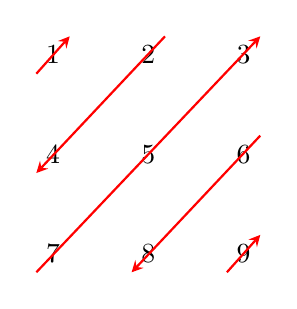
\begin{tikzpicture}
\matrix[row sep=8mm, column sep=8mm]
{
\node(1) {1}; & \node(2) {2}; & \node(3) {3}; \\
\node(4) {4}; & \node(5) {5}; & \node(6) {6}; \\
\node(7) {7}; & \node(8) {8}; & \node(9) {9};\\
};

\draw[red, thick, >=stealth, ->] (1.south west) -- (1.north east);
\draw[red, thick, >=stealth, ->] (2.north east) -- (4.south west);
\draw[red, thick, >=stealth, ->] (7.south west) -- (3.north east);
\draw[red, thick, >=stealth, ->] (6.north east) -- (8.south west);
\draw[red, thick, >=stealth, ->] (9.south west) -- (9.north east);
\end{tikzpicture}
\end{figure}
\end{flushleft}

\subsection{Matrix Trace}
在对角线上的元素的row和column index之和是相等的。

\setcounter{lstlisting}{0}
\begin{lstlisting}[style=customc, caption={Diagonal Element Has Same Sum Of Row and Column}]
vector<int> findDiagonalOrder( vector<vector<int>>& matrix )
{
    if( matrix.empty() || matrix[0].empty() )
    {
        return {};
    }

    size_t M = matrix.size();
    size_t N = matrix[0].size();

    //save the travese path
    vector<vector<int>> trace( M + N - 1 );

    for( size_t r = 0; r < M; ++r )
    {
        for( size_t c = 0; c < N; ++c )
        {
            auto x = r + c;

            trace[x].push_back( matrix[r][c] );
        }
    }

    vector<int> ans;
    ans.reserve( M + N );

    for( size_t i = 0; i < trace.size(); ++i )
    {
        if( i & 1 )
        {
            //odd sum: the direction is from top to bottom
            ans.insert( ans.end(), trace[i].begin(), trace[i].end() );
        }
        else
        {
            //even sum:  the direction is from bottom to top
            ans.insert( ans.end(), trace[i].rbegin(), trace[i].rend() );
        }
    }

    return ans;
}
\end{lstlisting}

\subsection{No Extra Memory}
\begin{itemize}
\item 有两个移动方向:向右上方移动,坐标变化为$[-1, 1]$,向左下方移动,坐标变化则为$[1, -1]$。
\item 可以根据坐标之和判断移动方向。奇数则向左下方移动,偶数向右上方移动。
\item 判断越界时,需要先判断row 或者column是否已经处于最大值的地方。因为每次越界,都要将column或者row increment。如果先判断row或者column是否为零,则会导致column或者row越界。
\end{itemize}

\setcounter{lstlisting}{0}
\begin{lstlisting}[style=customc, caption={Without Extra Memory}]
vector<int> findDiagonalOrder( vector<vector<int>>& matrix )
{
    if( matrix.empty() || matrix[0].empty() )
    {
        return {};
    }

    int M = static_cast<int>( matrix.size() );
    int N = static_cast<int>( matrix[0].size() );

    int r = 0;
    int c = 0;

    vector<int> ans( M * N );

    for( int i = 0; i < M * N; ++i )
    {

        ans[i] = matrix[r][c];

        int x = ( r + c );

        if( x & 1 )
        {
            //move down-left
            if( r == M - 1 )
            {
                //we need to check if row is in the bottom end first
                //cross boundary
                ++c;
            }
            else if( c == 0 )
            {
                //cross boundary
                ++r;
            }
            else
            {
                ++r;
                --c;
            }
        }
        else
        {
            //move up-right
            if( c == N - 1 )
            {
                //we need to check if column is at the right end first
                //cross boundary
                ++r;
            }
            else if( r == 0 )
            {
                //cross bounary
                ++c;
            }
            else
            {
                --r;
                ++c;
            }
        }
    }

    return ans;
}
\end{lstlisting}
%\include{499}
\end{document}